\PassOptionsToPackage{intlimits}{amsmath}

% \documentclass[journal]{IEEEtran}
\documentclass[twocolumn]{article}
\usepackage{etoolbox}
\usepackage{amsmath}
\usepackage[textwidth=7in,textheight=9.5in]{geometry} 
\usepackage{amsthm}
\usepackage{imakeidx}
\usepackage{transparent}
\usepackage[style=2,everyline=true,footnoteinside=true]{mdframed}
\usepackage{tabularx,booktabs}
\usepackage{commath}
\usepackage{esint} % various fancy integral symbols
\usepackage{tocloft}
\usepackage{etoc}
\usepackage{bm}
\usepackage{wrapfig}
\usepackage{multicol}
\usepackage{sepfootnotes}
\usepackage{xparse}
\usepackage[bottom]{footmisc}
\usepackage{amsfonts}
\usepackage[T1]{fontenc}
\usepackage[pdftex]{graphicx}
\usepackage{tikz}
\usepackage{pgfplotstable}
\usepgfplotslibrary{patchplots}
\usepackage{xcolor}
\usepackage{siunitx}
\usetikzlibrary{
	patterns,
	chains,
	backgrounds,
	calc,
	shadings,
	shapes.arrows,
	arrows,
	shapes.symbols,
	shadows,
	positioning,
	decorations.markings,
	backgrounds,
	arrows.meta,
	external
}

\usetikzlibrary{matrix}
\usetikzlibrary{fit}
\usetikzlibrary{shapes.geometric}
% \tikzexternalize[mode=list and make]
% \tikzexternalize
\usepackage{bbm}
\usepackage{relsize}
\usepackage{pgfplots}
\pgfplotsset{compat=newest}
\usepackage[edges]{forest}
\usepackage{adjustbox}
\usepackage{mathtools}
\usepackage{physics}
\usepackage{mleftright}
\NewDocumentCommand{\evalat}{sO{\big}mm}{%
  \IfBooleanTF{#1}
   {\mleft. #3 \mright|_{#4}}
   {#3#2|_{#4}}%
}
\usepackage{breqn}
\usepackage{subcaption}

\DeclareCaptionFormat{subfig}{#1#2#3}
\DeclareCaptionSubType{figure}
\captionsetup[subfigure]{format=subfig,labelsep=space,labelformat=parens}


% \usepackage[backend=bibtex, bibencoding=utf8, style=ieee]{biblatex}
\usepackage[backend=biber, bibencoding=utf8, style=ieee, backref=true]{biblatex}
\usepackage[hyperfootnotes=false,hyperindex=true]{hyperref}
\usepackage[utf8]{inputenc}
\makeindex

\setlength{\columnsep}{1cm}

\setlength{\cftsubsecindent}{0pt}% Remove indent for \subsection
\setlength{\cftsubsubsecindent}{10pt}% Remove indent for \subsubsection
\setlength{\cftparaindent}{20pt}% Remove indent for \paragraph
\setlength{\cftsubparaindent}{30pt}% Remove indent for \paragraph

\setcounter{secnumdepth}{5}
\setcounter{tocdepth}{5}
\renewcommand\thesection{\arabic{section}}
% \renewcommand\thesectiondis{\arabic{section}}

\renewcommand\thesubsection{\thesection.\arabic{subsection}}
% \renewcommand\thesubsectiondis{\thesectiondis.\arabic{subsection}}

\renewcommand\thesubsubsection{\thesubsection.\arabic{subsubsection}}
% \renewcommand\thesubsubsectiondis{\thesubsectiondis.\arabic{subsubsection}}

\renewcommand{\theparagraph}{\thesubsubsection.\arabic{paragraph}}
% \renewcommand{\theparagraphdis}{\thesubsubsectiondis.\arabic{paragraph}}

%\makeatletter
%\newcounter{subparagraph}[paragraph]
%\newcommand\subparagraph{%
%\@startsection
%    {subparagraph}    % counter
%    {5}                              % level
%    {\z@}                    % indent
%    {0.7ex plus .5ex minus 0ex}     % afterskip {0ex}
%    {0.7ex plus .5ex minus 0ex}     % afterskip {0ex}
%    {\normalfont\normalsize\itshape}
%}
%\makeatother
%\renewcommand{\thesubparagraph}{\theparagraph.\arabic{subparagraph}}
%\def\thesubparagraphdis{\theparagraph.\arabic{subparagraph}}

\makeatletter
\patchcmd{\@makecaption}
{\\}
{.\ }
{}
{}
\makeatother

\def\tablename{Table}
\renewcommand{\thetable}{\arabic{table}}
\newcommand{\ue}[1]{
	\begin{tikzpicture}[#1]
		\draw[fill = black] (.25ex,.25ex) circle (.3ex);
		\draw[thick] (.55ex,.25ex) -- (1.55ex,.25ex);
		\draw[fill = black] (1.85ex, .25ex) circle (.3ex);
	\end{tikzpicture}%
}

\newcommand{\newterm}[1]{\textit{#1}\index{#1}}

\newfootnotes{a}
\hypersetup{
	colorlinks,
	linkcolor={red!50!black},
	citecolor={blue!50!black},
	urlcolor={blue!80!black}
}
\addbibresource{quals.bib}
\definecolor{darkblue}{HTML}{1f4e79}
\definecolor{lightblue}{HTML}{00b0f0}
\definecolor{salmon}{HTML}{ff9c6b}

% Note that the amsmath package sets \interdisplaylinepenalty to 10000
% thus preventing page breaks from occurring within multiline equations. Use:
\interdisplaylinepenalty=0
\interfootnotelinepenalty=10000
\raggedbottom

% fix footnote rule from ieee
\def\footnoterule{
	\relax
	\kern-5pt
	\hbox to \columnwidth{\hfill\vrule width \columnwidth height 0.4pt}
	\kern4.6pt
}

\newcommand{\Xk}{X_k}
\newcommand{\Xkone}{X_{k+1}}
\newcommand{\bx}{\bm{x}}
\newcommand{\bX}{\bm{X}}
\newcommand{\bxi}{\bm{x}_i}
\newcommand{\delx}{\bx - \bxi}
\newcommand{\by}{\bm{y}}
\newcommand{\bY}{\bm{Y}}
\newcommand{\byi}{\bm{y}_i}
\newcommand{\dely}{\by - \byi}
\newcommand{\zbx}{Z(\bx)}
\newcommand{\zbxi}{Z(\bxi)}
\newcommand{\bb}{\bm{\beta}}
\newcommand{\hzbx}{\hat{Z}(\bx)}
\newcommand{\etal}{\textit{et al.}~}


\makeatletter
\renewcommand\subsubsection{%
	\@startsection
	{subsubsection}                 % type
	{3}                             % level
	{\z@}                    % indent
	%{3.5ex plus 1.5ex minus 1.5ex}  % beforeskip {0ex plus 0.1ex minus 0.1ex}
	{0.7ex plus .5ex minus 0ex}     % afterskip {0ex}
	{0.7ex plus .5ex minus 0ex}     % afterskip {0ex}
	{\normalfont\normalsize\itshape}% style
}
\makeatother
\makeatletter
\renewcommand\paragraph{%
	\@startsection
	{paragraph}                 % type
	{4}                             % level
	{\z@}                    % indent
	{0.7ex plus .5ex minus 0ex}     % afterskip {0ex}
	{0.7ex plus .5ex minus 0ex}     % afterskip {0ex}
	{\normalfont\normalsize\itshape}% style
}
\makeatother

\newlength\tocrulewidth
\setlength{\tocrulewidth}{1.5pt}
%\etocsettocstyle{\rule{\linewidth}{\tocrulewidth}\vskip0.5\baselineskip}{\rule{\linewidth}{\tocrulewidth}}
%\etocsettocstyle{\rule{.5\linewidth}{\tocrulewidth}\vskip0.5\baselineskip}{\rule{.5\linewidth}{\tocrulewidth}}
\etocsettocstyle{\medskip\hrule\medskip}{\medskip\hrule\medskip}
\etocsettocdepth{5}
\tikzset{
		greenarrow/.style={
				-latex,black!60!green,thick,solid
			},
		redarrow/.style={
				-latex,red,thick,solid
			},
		bluearrow/.style={
				-latex,blue,thick,solid
			},
		dot/.style = {
				circle,
				fill,
				minimum size=#1,
				inner sep=0pt,
				outer sep=0pt
			},
		dot/.default = 6pt
}

% colors
\definecolor{blue}{RGB}{38,139,210}
\definecolor{cyan}{RGB}{42,161,152}
\definecolor{violet}{RGB}{108,113,196}
\definecolor{red}{RGB}{220,50,47}
\definecolor{base01}{RGB}{88,110,117}
\definecolor{base02}{RGB}{7,54,66}
\definecolor{base03}{RGB}{0,43,54}

\definecolor{snowymint}{HTML}{E3F8D1}
\definecolor{wepeep}{HTML}{FAD2D2}
\definecolor{portafino}{HTML}{F5EE9D}
\definecolor{plum}{HTML}{DCACEF}
\definecolor{sail}{HTML}{A3CEEE}
\definecolor{highland}{HTML}{6D885A}

\tikzstyle{signal}=[arrows={-latex},draw=black,line width=1.5pt,rounded corners=4pt]

% RNN
\tikzstyle{block}=[draw=black,line width=1.0pt]
\tikzstyle{cell}=[style=block,draw=highland,fill=snowymint,
    rounded corners]
\tikzstyle{celllayer}=[style=block,draw,fill=portafino,
    inner sep=1pt,outer sep=0,
    minimum width=28pt, minimum height=14pt]
\tikzstyle{pointwise}=[style=block,ellipse,fill=wepeep,
    inner sep=1pt,outer sep=0, minimum size=12pt]

\def\iolen{24pt}
\def\intergape{2pt}

% MLP and CNN
\tikzstyle{netnode}=[circle, inner sep=0pt, text width=22pt, align=center, line width=1.0pt]
\tikzstyle{inputnode}=[netnode, fill=sail,draw=black]
\tikzstyle{hiddennode}=[netnode, fill=snowymint,draw=black]
\tikzstyle{outputnode}=[netnode, fill=plum,draw=black]

% Architecture
\def\layerwidth{90pt}
\def\layerheight{14pt}

\tikzstyle{layer}=[style=block, draw, fill=black!20!white,
    inner sep=1pt,outer sep=0, font=\footnotesize,
    text centered, 
    minimum width=\layerwidth, minimum height=\layerheight]

\tikzstyle{fc}=[style=layer, fill=blue!30!white]
\tikzstyle{conv}=[style=layer, fill=green!30!white]
\tikzstyle{activation}=[style=layer, fill=orange!30!white]
\tikzstyle{pool}=[style=layer, fill=red!30!white]
\tikzstyle{bn}=[style=layer, fill=cyan!30!white]
\tikzstyle{recurrent}=[style=layer, fill=purple!30!white]
\tikzstyle{softmax}=[style=layer, fill=yellow!30!white]
\tikzstyle{point}=[]
\tikzstyle{branch}=[coordinate]

\def\vlayerwidth{30pt}
\def\vlayerheight{3pt}
\def\vblockheight{28pt}

\tikzstyle{vlayer}=[minimum width=\vlayerwidth, minimum height=\vlayerheight]
\tikzstyle{vblock}=[minimum width=\vlayerwidth, minimum height=\vblockheight, text width=1cm, align=center]


% Precision, Recall
\colorlet{fn}{gray!90!green!30!white}
\colorlet{tp}{green!40!white}
\colorlet{fp}{red!40!white}
\colorlet{tn}{gray!90!red!20!white}
\newtheorem{theorem}{Theorem}

%! Suppress = GatherEquations
% introduction
\anotecontent{vbsuper}{We will often use the verb form ``to super resolve'' in order to denote the use of one or more such methods.}
\anotecontent{rayleighscriterion}{The amplitude of the diffraction pattern (known as the Airy pattern) of a monochromatic point source through a circular aperture is given by \[I(\theta)\coloneqq I_{0}\left[{\frac {2J_{1}(ka\sin \theta )}{ka\sin \theta }}\right]^{2}\] where \(I_0\) is peak intensity (at the center), \(k=\frac{2\pi}{\lambda}\) is the wavenumber of the light, \(\theta\) is the angle of observation, and \(J_1\) is the Bessel function of the first kind of order one \cite{goodman2005introduction}.
	%
	It is maxima/minima of this function that Rayleigh's criterion concerns.}
\anotecontent{shotnoise}{The number of photons incident on a sensor element is distributed according to a Poisson distribution (arrivals are independent and their rate is constant). For a small number of photons the variance in total arrivals (i.e., image brightness) is high.}
\anotecontent{satelliteoptics}{Rayleigh's criterion implies that the angular resolution \(R\) of a telescope with optical diameter \(D = 2.4\text{m}\) observing visible light (\({\sim}500\text{nm}\)) is approximately \cite{doi:10.1080.14786447908639684} \[R  \approx 1.220\frac{\lambda}{D} = 1.220 \frac{500\text{nm}}{2.4\text{m}} \approx 0.06\text{arcsec}\] From an altitude of 250 km this corresponds to a ground sample distance of 6cm.
	%
	This loss of resolving power is further exacerbated by refraction through turbulent atmosphere \cite{Fried:66}.}
\anotecontent{subpixel}{For example when a point source wholly captured by one sensor element shifts to distributing energy equally amongst that same element and a direct adjacent.}

% background
\anotecontent{lexico}{Consider an \(N\) row \(\times\) \(M\) column image \(X(n, m)\).
	%
	The column-major vectorization \(bm{x}\) of the image is the \(NM\) length vector defined as \(\bm{x}(Mm + n) = X(n, m)\).}
\anotecontent{patch}{\(m \times m\) pixel window, e.g. \(3 \times 3\).}
\anotecontent{tensor}{A multidimensional array. Not to be confused with the algebraic object.}
%\anotecontent{deep-depletion}{The depletion layer is the region at the Si-SiO\(_2\) interface that is characterized by few charge carriers (electrons and holes) that occurs when a gate voltage higher than the flat-band voltage is applied. Deep-depletion is characterized by a depletion region width that is greater than that at equilibrium \cite{semiconductorbook}.}
%\anotecontent{inversion}{The term inversion means that the surface is inverted from P type to N type, or electron rich. This process is a slow thermal equilibration \cite{ccdarkcurrent}, is called dark current and at various temperatures/exposure times is a source of noise.}
\anotecontent{nyquist}{Twice the frequency of the lowest frequency component in the image. Sampling at a rate below this leads to aliasing of high frequency components as low frequency components.}
\anotecontent{depletion}{By applying a positive voltage to the gate holes are repelled and migrate through the body to ground.
	%
	This leaves a depleted region near the Si-SiO\(_2\) interface that acts as an insulator.}
\anotecontent{buriedchannel}{Buried channel as distinct from surface channel.
	%
	In surface channel the signal charge is stored at the Si-SiO\(_2\) interface, which can lead to charge trapping during the charge transfer process \cite{Bass:2009:HOT:1594759}.}
\anotecontent{ntype}{Semiconductors are classified as either \textit{n-type} or \textit{p-type}, the former being doped with negative charge carriers and the latter being doped with positive charge carriers (holes).}
\anotecontent{ccd}{CCD arrays, for example, employ \(2\times 2\) or \(3\times 3\) pixel binning, which is the practice of collapsing windows of pixels down to one pixel.}
\anotecontent{pnjunction}{The interface between a p-type semiconductor and a n-type semiconductor.}
\anotecontent{reversebias}{With the p-type material at a lower voltage than the n-type.
	%
	This causes both the holes and the electrons to flow away from the junction creating a depletion zone.}
\anotecontent{bolometer}{Late 19th century: from Greek bolē `ray of light' + -meter.}
\anotecontent{mems}{Micro-electro-mechanical systems.}
\anotecontent{fabryperot}{An optical cavity made from two parallel reflecting surfaces that passes light only when it is in resonance with the cavity.}
\anotecontent{thermistor}{An element with an electrical resistance that is a function of its temperature.}
\anotecontent{innerphotoelectric}{The photoelectric effect is the emission of electrons when light hits a material.
	%
	The inner photoelectric effect is that phenomenon in the bulk matter of semiconductors.}
\anotecontent{otf}{The optical transfer function is the spatial Fourier transform of the point spread function (the impulse response) of the optics.
	%
	Spatial here means periodic in space rather than in time.}
\anotecontent{coma}{Off-axis point sources appearing to have a tail (coma), due to variation in magnification in the image of the aperture stop.}
\anotecontent{dispersion}{A well known example of this phenomenon is the cover of Pink Floyd's classic album The Dark Side of the Moon.}
\anotecontent{fnumber}{The ratio of the system's focal length to the diameter of the aperture.}
\anotecontent{registration}{The process of aligning two or more images of the scene on a common pixel grid.}
%registration
\anotecontent{scalepyramid}{No pun intended.}
\anotecontent{threshold}{Set everything below a threshold to zero.}
\anotecontent{nms}{Pick the maximum in a neighborhood and set all other values to zero.}
\anotecontent{log}{The Laplacian of an image \(X\) is \(L(x,y) = \partial_x^2 X + \partial_y^2 X\).
	%
	Since in practice this approximates a noisy signal (second derivative), smoothing by a Gaussian is a necessary prerequisite.
	%
	Therefore the Laplacian of Gaussians (\(LoG\)) filter is the Laplacian composed with the Gaussian: \begin{equation*} LoG(x,y, \sigma) \coloneqq -\frac{1}{\pi \sigma^4}\left[ 1 - \frac{x^2+y^2}{2\sigma^2} \exp \left\{ - \frac{x^2+y^2}{2\sigma^2} \right\} \right]
	\end{equation*}}
\anotecontent{smallcurvature}{The ratio of the eigenvalues of the spatial Hessian of \(D\) (i.e., only along dimensions \(x,y\)).
	%
	In fact a quantity not unlike eqn.~\eqref{eqn:strength} is computed in order to save having to explicitly find eigenvalues.}
\anotecontent{hog}{The histogram of gradient orientations (polar angle) in a pixel window.}
\anotecontent{kdtree}{\(k\)-d trees \cite{Bentley:1975:MBS:361002.361007}, short for \(k\)-dimensional trees, are data structures that partition space efficiently in order that searching the data structure, insertion into the data structure, and deletion from the data structure are all, on average, \(O(\log n)\) time operations (where \(n\) is the number of nodes in the tree at the time of the operation).}
\anotecontent{ransac}{Random Sample Consensus (RANSAC) is a method used to estimate parameters of a model given outliers.
	%
	In this case Zahra \etal use RANSAC at the transform estimation step to eliminate falsely matched keypoint pairs.
	%
	RANSAC iterates by repeatedly random sampling the putative matching keypoint pairs and fitting a transform model.
	%
	At a given iteration the fitted transform model is tested against the heldout keypoint pairs and evaluated (according to goodness of fit on a subset called the \textit{consensus set}).}
\anotecontent{gridsearch}{Searching a space by taking regular incremental steps along each dimension. For example, search \(U \subset \mathbb{R}^2\) by checking all \(x = \Delta x + x_0, y = \Delta y + y_0\) for \((x_0, y_0) \in U\) and for fixed \(\Delta x, \Delta y\).}
\anotecontent{fouriershift}{If \(\mathcal{F}\{\left[ x_n \right] \}_{k}=X_{k}\) is the \(k\)-th frequency component of the discrete signal
\(\left[ x_n \right]\) then shifting \(\left[ x_n \right]\) by \(m\) steps implies
\[
	\mathcal{F}\left\{\left[ x_{n-m} \right]\right\}_{k} = X_{k}\cdot e^{-{\frac {i2\pi }{N}}km}
\]
}
\anotecontent{hadamard}{
	\[
		\begin{bmatrix}
			a_{11} & a_{12} \\
			a_{21} & a_{22} \\
		\end{bmatrix}\odot \begin{bmatrix}
			b_{11} & b_{12} \\
			b_{21} & b_{22} \\
		\end{bmatrix} \coloneqq
		\begin{bmatrix}
			a_{11}\,b_{11} & a_{12}\,b_{12} \\
			a_{21}\,b_{21} & a_{22}\,b_{22} \\
		\end{bmatrix}
	\]
}
\anotecontent{shannon}{
	Shannon entropy can be interpreted as the average number of bits \(L\) necessary to encode a random variable \(X\) distributed according to distribution \(P\).
	%
	It is defined as
	\[
		H(X)\coloneqq\sum{P(x)\log\left[\frac{1}{P (x)}\right]}
	\]
	i.e., \(P(x_i) = 1/2^L\) where \(L\) is the number of bits.
}
\anotecontent{kde}{Alternatively known as Parzen windowing, the kernel density estimator \(\hat{P}\) of a distribution \(X\sim P\) given a set of points \(\left\{ x_1, x_2, \dots, x_n \right\}\) is defined as
	\[
		\hat{P}(x) \coloneqq {\frac {1}{nh}}\sum _{i=1}^{n}K\left( \frac {x-x_{i}}{h} \right)
	\]
	where \(K\) is a kernel (e.g. Gaussian) and \(h\) is the \textit{kernel bandwidth}.
}
\anotecontent{convexhull}{A convex combination of points \(x_1, x_2, \dots, x_n\) is all \(\alpha _{1}x_{1}+\alpha _{2}x_{2}+\cdots +\alpha _{n}x_{n}\) where \( \alpha _{i}\geq 0\) and \(\alpha _{1}+\alpha _{2}+\cdots +\alpha _{n}=1\).
%
The convex hull of a set of points \(X\) is the set of all convex combinations of points in \(X\).
%
Figuratively one can imagine stretching a rubber band such that it contains all points in \(X\).}
\anotecontent{completegraph}{A graph in which each pair of vertices is connected by an edge.}
\anotecontent{homogeneous}{
	With \((x,y)\) a pixel coordinate, transformations \(T\) in homogeneous coordinates operate on \((x,y,1)\): if
	\(
	(a,b,c) = (x,y,1)\cdot T
	\)
	then the transformed pixel coordinate
	\(
	(x',y') = \frac{1}{c} (a,b)
	\).
}
\anotecontent{advection}{Advection is the transport of a substance, or properties thereof, by bulk flow of a fluid. The substance, or properties thereof, are \textit{advected} by the flow and are considered \textit{conserved}. In general, the fluid flow is described by a vector field \(\mathbf{u}\) (called velocity) and the substance or property is described by a scalar field \(\psi\) (variously called distribution, concentration, or density). The canonical example is the advection of ink by flowing water.}
\anotecontent{stokes}{
	The integral of a differential form \(\omega\) on the boundary of some orientable manifold \(\Omega\)  is equal to the integral of its exterior derivative \(\dif \omega\) on \(\Omega\), i.e
	\[
		\oint\limits _{\partial \Omega }\omega =\int\limits _{\Omega }\dif\omega
	\]
	In this instance \(\Omega = R\), \(\omega = \mathbf{j} \cdot \mathbf{n}\, \dif l \) and \( \dif \omega = \nabla \cdot \mathbf{j}\, \dif R\).
}
\anotecontent{tvloss}{ Total variation is equivalent to the integral of the gradient magnitude:
\[
	\abs{u}_{\operatorname {TV}}=\int\limits\abs{\nabla u}
\]
}
\anotecontent{indicator}{The indicator (or characteristic) \(\mathbbm{1}_{[a,b)}\) function is 1 on the interval \([a,b)\) and 0 otherwise.}
\anotecontent{vectorspace}{A set whose members (\textit{vectors}) can be decomposed as linear combinations of elementary elements (a \textit{basis}).}
\anotecontent{splinecontconstr}{Note that even though a \(d\)-degree polynomial has \(d\) derivatives we only require agreement at the first \(d-1\) derivatives (and continuity itself). This is owing to the fact that if we required all \(d\) derivatives to agree the number of degrees of freedom would be \((n(d+1) - (n-1)(d+1) = d+1\) and therefore the spline would no longer be a piecewise polynomial but simply a polynomial (of degree \(d\)).}



%classical
\anotecontent{delauney}{The Delaunay triangulation for a set of points \(P\) is a triangulation such that no point in \(P\) is inside the circumcircle of any triangle in the triangulation. Equivalently it is the triangulation that maximizes the minimum angle of all of the triangles in the triangulation.}
\anotecontent{estiminterp}{This blurring of the distinction between interpolation and estimation is to be expected since estimation is a type of regression.}
\anotecontent{gp}{A Gaussian process is a sequence of random variables such that any finite subset is distributed multivariate Normal.}
\anotecontent{lsi}{In analogy with Linear Time Invariant (i.e., linear and constant in space).}
\anotecontent{lrpixel}{An LR pixel is one sampled from an LR image and embedded in the HR grid.
	%
	An HR pixel is a pixel in the HR grid.}
\anotecontent{vectorize}{
	\begin{multline*}
		\text{vec}\left(
		\begin{bmatrix}
				a_{11} & a_{12} & \cdots & a_{1n} \\
				a_{21} & a_{22} & \cdots & a_{2n} \\
				\vdots & \vdots & \ddots & \vdots \\
				a_{m1} & a_{m2} & \cdots & a_{mn}
			\end{bmatrix}
		\right) = \\
		\left[a_{11}, \mathellipsis, a_{m1}, a_{12}, \mathellipsis, a_{m2}, \mathellipsis, a_{1n} \mathellipsis a_{mn}\right]
	\end{multline*}
}
\anotecontent{noise}{Noise here doesn't necessarily mean unwanted high frequency variation but simply a source of randomness.
	%
	This is in close affinity with how generative machines such as variational auto-encoders and generative adversarial networks are understood.}
%
\anotecontent{gpassumptions}{Namely \(\bm{y}_1\) is distributed \((0, W)\)-Normal and independent of \(\eta_1\).}
\anotecontent{kalmanprediction}{This is better understood in the more general linear dynamic systems case where \(\bm{y}_k = A_k\cdot\bm{y}_k + B_k \cdot \bm{u}_k + \varepsilon_k\) and \(B_k \cdot \bm{u}_k\) is known as controlled input.
	%
	Then the prediction includes a \(B_k \cdot \bm{u}_{k-1}\) term and the Kalman gain effectively mediates between controlled and uncontrolled inputs.
}
\anotecontent{hmrf}{A Markov Random Field (MRF) is a collection of random variables \(x_i, y_j, \mathellipsis\) with conditional dependence represented by pairings and satisfying the \textit{pairwise Markov} property: any two random variables that aren't paired are conditionally independent of each other given (conditioned on) all other variables.
	%
	A \textit{Hidden} Markov Random Field is simply a MRF where some of the random variables aren't observed.
}
\anotecontent{locallinear}{An LR patch \(x_i\) on the LR manifold and its neighbors \(x_j, x_k, \mathellipsis\) lie in a locally linear subspace of the manifold.}
\anotecontent{forest}{A tree is a graph in which any pair vertices is connected by exactly one or zero edges. A forest is a disjoint collection of trees.}
\anotecontent{positivedef}{A symmetric real matrix \(Q\) is positive definite if \(\bm{y}^T Q \bm{y} > 0 \) for all non-zero \(\bm{y}\).}
\anotecontent{conjugategradients}{Two vectors \(\bm{u}, \bm{v}\) are conjugate with respect to \(G\) if \(\bm{u}^T G \bm{v} = 0\).
	%
	Conjugate gradient descent is gradient descent but with conjugate gradients (it has better convergence properties).
}
\anotecontent{illcondition}{The condition number \(\kappa\) of a function is a measure of how sensitive it is to small perturbations; for a matrix \(G\) it is defined \(\kappa (G) \coloneqq \sigma_{\max}(G)/\sigma_{\min} (G)\) where \(\sigma_{\max}(G), \sigma_{\min} (G)\) are the maximum and minimum singular values of \(G\) respectively.}
\anotecontent{precondition}{A preconditioner of a matrix \(G\) is an approximation of \(G\) that has a better condition number.
	%
	Nguyen \textit{et al.} propose a preconditioner with singular values clustered around 1 in order that \(\kappa(G) \approx 1\).}
\anotecontent{gradientoperator}{Let \(u = (1,2,1)\) and \(v = (1,0,-1)\) then \(h = uv^T\) is the first order Sobel filter and \(\nabla Y = \left( h \ast Y, h^T \ast Y \right)\).}
\anotecontent{boundedvariation}{\(f(x)\) is of bounded variation on interval \(\left[ a,b \right]\) if over all partitions \(\mathcal{P}\) of \(\left[ a,b \right]\)
	\[
		\sup_{P \in \mathcal{P}}\sum_{i=0}^{n_P-1} \lvert f(x_{i+1})-f(x_i) \rvert\, <\infty
	\]
}
\anotecontent{beliefpropagation}{An efficient way to compute marginals of joint probabilities that have structure by reusing partial sums (i.e., passing messages) \cite{Yedidia2003jan1}.}
\anotecontent{manifold}{A collection of points that locally resembles Euclidean space.}
\anotecontent{manifoldlearning}{Dimensionality reduction.}
\anotecontent{pun}{No pun intended.}
\anotecontent{overcompletedictionary}{A collection of vectors (known as \textit{atoms}) that spans a space but is also linearly dependent.}
\anotecontent{nphard}{Problems in NP are those which are unknown to have a deterministic polynomial time solutions.
	%
	An NP-hard problem admits a polynomial time reduction from any problem in NP (colloquially they are as hard as any problem in NP).}
\anotecontent{firstordergaussian}{The first derivative of the Gaussian expressed as a filter: \(\left[ -2,-1,0,1,2 \right]\).}

% ann
\anotecontent{ann}{Artificial neurons are loosely inspired by the spiking neuron model of biological neurons, where dendrites correspond to inputs, the soma corresponds to a linear sum of inputs, and axons corresponds to the activation function.}
\anotecontent{bias}{The semantics of bias are inherited from from statistics, where the bias of an \textit{estimator} is the extent to which the estimator, on average, differs from the value being estimated. Therefore, if we regard an artificial neuron as an estimator (a nonlinear regression), we see that the constant term \(b\) indeed determines its bias.
}
\anotecontent{xor}{Exclusive-Or \(\operatorname{XOR}(a,b)\) is a Boolean function (maps \(\{0,1\}\) to \(\{0,1\}\)) defined to be 1 when \(a \neq b\) and 0 otherwise.}
\anotecontent{backprop}{Backprop itself is a particular instance of a general technique called automatic differentiation (AD). AD computes exact derivatives of functions in either \textit{forward accumulation} or \textit{reverse accumulation} \cite{linnainmaa1976taylor}. Backprop corresponds to reverse mode. In reverse mode the dependent variable \(y\) to be differentiated is fixed and the derivative is computed with respect to each sub-expression \(z_i\) recursively:
	\begin{multline*}
		{\frac  {\partial y}{\partial w}}={\frac  {\partial y}{\partial z_{1}}}{\frac  {\partial z_{1}}{\partial w}}=\left({\frac  {\partial y}{\partial z_{2}}}{\frac  {\partial z_{2}}{\partial z_{1}}}\right){\frac  {\partial z_{1}}{\partial w}}=\\\left(\left({\frac  {\partial y}{\partial z_{3}}}{\frac  {\partial z_{3}}{\partial z_{2}}}\right){\frac  {\partial z_{2}}{\partial z_{1}}}\right){\frac  {\partial z_{1}}{\partial w}}=\cdots 
	\end{multline*}
}
\anotecontent{universapprox}{Given enough layers and neurons ANNs with nonlinear activations are able to represent functions of arbitrary complexity. Conversely, sans a nonlinear activation function, ANNs are unable to represent functions as simple as even \(\operatorname{XOR}\).}
\anotecontent{learn}{To learn, in this context, means to approximate a function that effectively performs a task. For example in the case of an object recognition task, learning entails approximating a function that outputs high values when an object is recognized and low values otherwise.}
\anotecontent{largeparams}{OpenAI’s Generative Pre-trained Transformer (GPT) \cite{radford2018improving} natural language processing (NLP) network has approximately 150 million parameters (and takes 8 GPU-months of non-stop training).}
\anotecontent{kldiv}{The Kullback–Leibler divergence of two probability distributions \(P,Q\) with densities \(p, q\) is defined
	\begin{equation*}
		\operatorname{D}_{\text{KL}}(P\parallel Q)\coloneqq\int\limits _{-\infty }^{\infty }p(x)\log \left({\frac {p(x)}{q(x)}}\right)\,dx
	\end{equation*}
Note that \(\operatorname{D}_{\text{KL}}\) is not symmetric and therefore not a true distance measure. Fortunately it can be symmetrized:
\begin{equation*}
	\operatorname{JSD}(P\parallel Q)\coloneqq{\frac  {1}{2}}\operatorname{D}_{\text{KL}}\left(P\bigg\| {\frac  {1}{2}}(P+Q)\right)+{\frac  {1}{2}}\operatorname{D}_{\text{KL}}\left(Q\bigg\| {\frac  {1}{2}}(P+Q)\right)
\end{equation*}
In this form it is called the Jensen–Shannon divergence and is a true distance measure between probability distributions.
}
\anotecontent{minimax}{Strictly speaking mini-max is a decision rule followed by each player of a game --- a decision rule that leads to minimizing the possible loss for a worst case (maximum loss) scenario.}
\anotecontent{uniformconv}{A sequence of functions \(F_n\), \textit{uniformly converges} to \(f\) on a bounded interval \(I\) if given some \(\varepsilon > 0\) there exists \(n\) such that 
\[
	\abs{ F_n( x ) - f ( x ) } < \varepsilon
\]
for all \(x \in I\). Note the order of the quantifiers: there should be \textbf{one} \(n\) that satisfies the constraint at a given precision \(\varepsilon\) for \textbf{all} \(x \in I\) simultaneously.
}
\anotecontent{annealing}{Learning rate annealing imposes a scheduled decay of the learning rate \(\alpha_i\) over time. The intuition being that initially, prior to identifying a minimum, one can afford to take optimistically large steps \(\Delta w_i\) in parameter space but over time one should become more conservative in order to hone in on an identified minimum. Typically the annealing schedule is such that the learning rate out starts out large and is reduced by an order of magnitude (i.e., a factor of 10) every \(M\) epochs (where \(M\) is a divisor of the total number of epochs that one will train for).}
\anotecontent{gradclip}{Exploding gradients is the opposite of vanishing gradients: gradients become so large that weights become unstable. That is, weight updates become large and oscillate around a minimum. Gradient clipping constrains \(\pd{L}{w_i}\) to be within a narrow range around 0; Kim \etal constrain the gradient to be within \(\left[ -\frac{\theta}{\alpha_i}, \frac{\theta}{\alpha_i} \right]\) for some small \(\theta\).}
\anotecontent{ntire}{The performances of various techniques on SISR and MISR tasks are evaluated at a competition held at the annual New Trends in Image Restoration and Enhancement (NTIRE) workshop. The competition \cite{nah2019ntire} has two tracks: a clean track that only assumes down-sampling test cases and a blur (or natural) track that assumes motion blur (in an effort to approximate real conditions). Many teams compete in both tracks.}

% conclusions
\anotecontent{transfer}{Given a source domain and target domain, transfer learning sets out to accelerate learning for a task over the target domain using learning already performed for a task over the source domain.}
\anotecontent{tremor}{For example Physiologic tremor in the case of cell phone cameras. Physiologic tremor is a low amplitude tremor of a limb that presents at approximately 10Hz. It occurs in normal, healthy individuals.}
\anotecontent{rl}{Reinforcement Learning is a paradigm of machine learning based on principles of operant conditioning, i.e., using punishment and reward.}
\anotecontent{rnn}{A Recurrent Neural Network (RNN) models time dependencies in sequences of data.}

% appendix
\anotecontent{diracdelta}{A generalized function is a function that can only be integrated against. Let 
\begin{equation*}
	\delta_\epsilon(x) \coloneqq \frac{1}{\epsilon \sqrt{\pi}}	e^{-x^2/\epsilon^2}
\end{equation*}
Then for any continuous \(\phi(x)\)
\begin{equation*}
	\lim_{\epsilon\rightarrow 0} \left[\int\limits_{-\infty}^{\infty} \phi(x)\delta_{\epsilon}(x-x_0) \right] = \lim_{\epsilon\rightarrow 0} \left[ \phi(x_0)\int\limits_{-\infty}^{\infty} \delta_{\epsilon}(x-x_0) \right] = \phi(x_0)
\end{equation*}
and hence \(\delta(x)\) is defined as the limit of this behavior
\begin{equation*}
	\int\limits_{-\infty}^{\infty} \phi(x)\delta(x-x_0) = \phi(x_0)
\end{equation*}
}
\usepackage{fnbreak}
\begin{document}
\title{Super Resolution for Automated Target Recognition}
\author{Maksim Levental}
\maketitle

\begin{abstract}
	Super resolution is the process of producing high-resolution images from low-resolution images while preserving ground truth about the subject matter of the images and potentially inferring more such truth.
	%
	Algorithms that successfully carry out such a process are broadly useful in all circumstances where high-resolution imagery is either difficult or impossible to obtain.
	%
	In particular we look towards super resolving images collected using longwave infrared cameras since high resolution sensors for such cameras do not currently exist.
	%
	We present an exposition of motivations and concepts of super resolution in general, and current techniques, with a qualitative comparison of such techniques.
	%
	Finally we suggest directions for future research.
\end{abstract}
% \newpage
\tableofcontents

\section{Introduction}\label{sec:introduction}
\noindent{\vrule width \columnwidth height 0.4pt}

Super-resolution (SR) is a collection of methods\anote{vbsuper} that augment the resolving power of an imaging system.
%
Here, and in the forthcoming, by resolving power we mean the ability of an imaging device to distinguish distinct but proximal objects in a scene.
%
If such objects are modeled as point sources of light then the resolving power of the imaging system is defined by Rayleigh's criterion: two point sources are considered \newterm{resolved} when the first diffraction maximum\anote{rayleighscriterion} of one point source coincides (at most) with the first minimum of the other (see figure~\ref{fig:rayleigh}).
\begin{figure}[!htbp]
	\center
	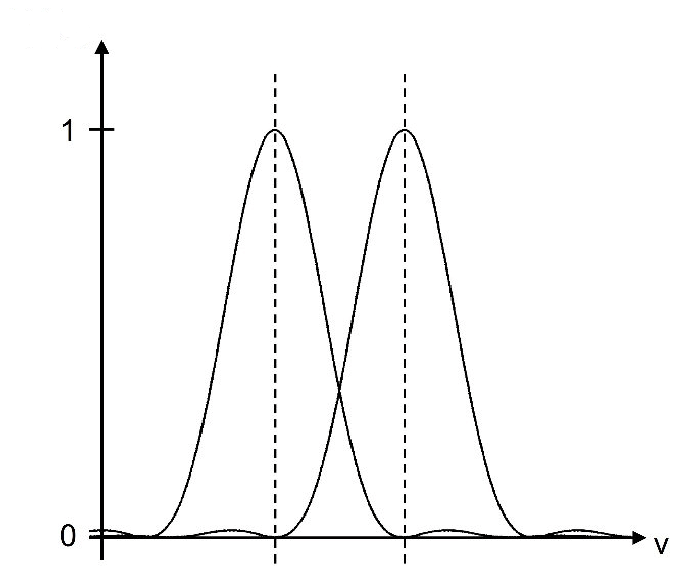
\includegraphics[width=\linewidth,keepaspectratio]{figures/classical/rayleigh.png}
	\caption{Rayleigh's criterion. Dashed lines indicate diffraction maxima and minima \cite{rayleigh}.}
	\label{fig:rayleigh}
\end{figure}

SR techniques yield high-resolution (HR) images from one or more observed low-resolution (LR) images by restoring lost fine details and reversing deterioration produced by imperfect imaging systems.
%
In the case where a single LR source image is used to construct the HR correspondent, the techniques are referred to as single-image-super-resolution (SISR) techniques.
%
These techniques typically operate either by constructing a mapping from low resolution patches\anote{patch} to higher resolution patches or by estimating the HR image given the LR image.
%
In the case when multiple LR source images are used to construct a single HR correspondent, the techniques are referred to as multiple-image-super-resolution (MISR) techniques.
%
MISR techniques rely on non-redundant and pertinent information in multiple images of the same scene (see figure~\ref{fig:misr}).
\begin{figure}[!htbp]
	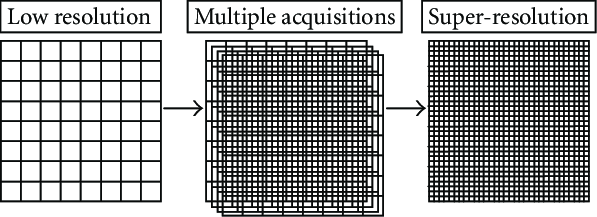
\includegraphics[width=\linewidth,keepaspectratio]{figures/classical/misr.png}
	\caption{Multiple image super resolution. Multiple low resolution images are superposed on a higher resolution grid in order to recover non-redundant information \cite{misr}.}
	\label{fig:misr}
\end{figure}
%
Note that for such information to exist there should be sub-pixel\anote{subpixel} shifts in either the imaging system or the scene between consecutive images.

For typical imaging use-cases higher resolutions are
desirable in and of themselves and as inputs to later image processing transformations that can further degrade image quality.
%
In theory the resolving power of an imaging system is primarily determined by the number of independent sensor elements that comprise that imaging system (each of which collects a component of the ultimate image).
%
Naturally then, a way to increase the resolution of such a system is to increase the density of such sensor elements per unit area.
%
Unfortunately, and counter-intuitively, since the number of photons incident on each sensor decreases as the sensor shrinks, shot noise\anote{shotnoise} thwarts that idea.
%
Furthermore, while sensor density is primary, secondary effects limit resolution as well.
%
For example, the point spread of a lens (distortion of a point source due to diffraction), chromatic aberrations (distortion due to differing indices of refraction for differing wavelengths of light), and motion blur all work to obscure or erase details from the image.


In domains such as satellite/aerial photography, medical imaging, and facial recognition,
high-resolution reconstruction of low-resolution samples is eminently useful since ab-initio acquisition of high-resolution images is either logistically difficult or impossible.
%
For example, in the case of satellite imagery, acquisition of high-resolution imagery is primarily hampered by optics and physics\anote{satelliteoptics}.
%
In contrast, in the case of medical imaging, where patient exposure time needs to be minimized \cite{doi:10.1002.cmr.a.21249}, the primary challenges are logistics and access to repeat collection opportunities.

The benefits of enhancing images using SR techniques include not only more pleasing or more readily interpretable images for human consumption, but higher quality inputs for automated learning systems as well.
%
Indeed this is our ultimate goal --- not super-resolution per se but super-resolution in the service of improved object detection performance for longwave-infrared (LWIR) imagery.
%
Towards that end, we do not consider hardware solutions for increasing the resolution of an imaging system.
%
We instead take low resolution images as given produce of a fixed imaging system and explore techniques that allow for ex post facto recovery or inference of precise details.
%
This necessarily constrains techniques under consideration to be algorithmic in nature and software in practice.

The rest of this survey is outlined as follows: section~\ref{sec:background} introduces imaging systems, notation, and the mathematical framework for the proceeding sections, section~\ref{sec:registration} surveys image registration techniques (a necessary pre-processing step for MISR), section~\ref{sec:classical-algorithms} surveys classical techniques (those that do not employ neural networks), section~\ref{sec:neural-networks} surveys neural network techniques with heavy emphasis on deep learning, and finally section~\ref{sec:conclusions} concludes with a brief discussion of future research directions.

\newpage
\subsection{Imaging systems}\label{subsec:imaging-systems}
\begin{figure}
	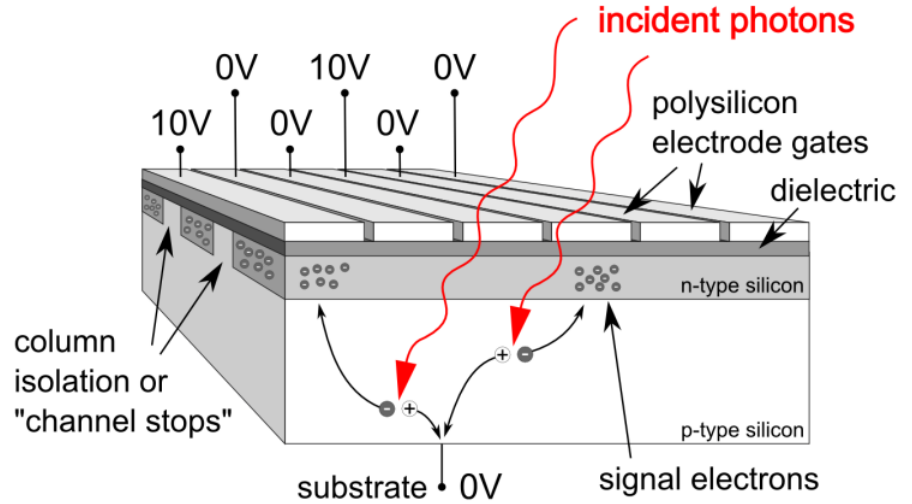
\includegraphics[width=\linewidth,keepaspectratio]{figures/background/bccd.png}
	\caption{CCD buried channel MOS capacitor\cite{finaltestguideline}}
	\label{fig:mos-cap}
\end{figure}
We begin with a practical discussion of imaging systems.
%
An imaging sensor is a device that converts an optical image into a digital signal.
%
Charge-coupled devices (CCD) and complementary metal-oxide-semiconductor (CMOS) devices are the most common imaging sensors;
%
CCDs have better performance while CMOS devices are newer and less expensive.
%
A third type that's of particular interest to us is the microbolometer, which is used as a sensor in thermal cameras.
\subsubsection{CCD Devices}
CCDs consist of densely packed two-dimensional arrays of buried channel\anote{buriedchannel} MOS capacitors (see figure~\ref{fig:mos-cap}) with an individual MOS capacitor being the fundamental photon detecting element.
%
Individual MOS capacitors are biased by a gate voltage such that a potential well is produced in the n-type silicon (referred to as the n-channel).
%
This potential well acts as a storage system for charge induced by the inner photoelectric effect\anote{innerphotoelectric}.
%
When photons are incident on a MOS capacitor some of the photons are absorbed, some are scattered, and some are transmitted.
%
Those photons that are transmitted interact with electrons in the valence band of the silicon exciting them into the conduction band, and thereby create electron-hole pairs that either diffuse or recombine.
%
For high-quality silicon, the lifetime of such a pair is several milliseconds (before recombination)\cite{scientificccd}.
%
The electrons of the electron-hole pairs that do not recombine diffuse into the potential well, while the holes migrate to the grounded substrate (i.e. out of the sensor).
%
Electrons created in this way are called \textit{photoelectrons}.

CCD arrays consist of two sub-arrays: an image section and a readout section (see figure~\ref{fig:ccd-array}).
%
The image section is arranged with every third stripe of electrode tied electrically to form three sets of equipotentials.
\begin{figure}
	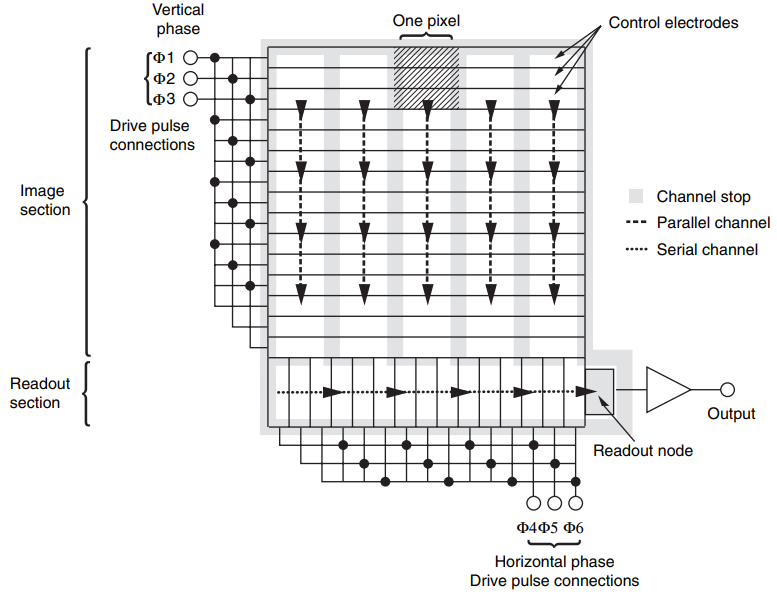
\includegraphics[width=\linewidth,keepaspectratio]{figures/background/ccd_array.png}
	\caption{CCD array\cite{pawley1995handbook}}
	\label{fig:ccd-array}
\end{figure}
%
In figure~\ref{fig:ccd-array} these equi-potentials are labeled $\Phi1, \Phi2, \Phi3$, and taken together constitute a vertical register (VR).
%
They function to move the collected photo-electrons down one electrode line at a time, using charge coupling, while the channel stops function to prevent diffusion of charge across channels.
%
The VR mechanism that shifts collected charge operates as follows:
\begin{framed}
\begin{enumerate}
	\item Suppose initially there's a collection of photo-electrons on each channel at $\Phi1$ and only $\Phi1$. Note this means $\Phi2, \Phi3$ are at $0$v (again just as in figure~\ref{fig:mos-cap}).
	\item $\Phi2$ is positively biased to $10$V. This diffuses the collection of charge under both $\Phi1$ and $\Phi2$.
	\item $\Phi1$ is set to $0$v. This concentrates the collection of charge under $\Phi2$.
	\item The same is repeated with $\Phi2, \Phi3$ and $\Phi3, \Phi1$.
	\item The entire process repeats thereby shifting the charge three lines (or one pixel row) at a time.
\end{enumerate}
\end{framed}
At the bottom of the image section $\Phi3$ transfers all signal charges to the horizontal register (HR) which functions much like the VR except faster: the HR must transfer every line of pixels independently of all other lines to the read-out node.
%
An obvious challenge faced by this system is how to prevent errant charge from accumulating out of sync with the shift process i.e. how to prevent new photoelectrons from being produced at intermediate lines while far lines are being shifted.
%
The solution is to have interstitial dedicated shift channels in between columns of sensors, with the shift channels being masked off from exposure to light.
%
This type of reading is called \textit{interline transfer} because the accumulated charge is first moved one line over, into the shift channels.
%
Naturally interline transfer shrinks photosensitive area by half and despite possible solutions (e.g micro-lenses being used to focus most of the light onto the unmasked sensors) this is one of the drawbacks of CCDs that CMOS imaging systems do not share.
\subsubsection{CMOS Devices}
CMOS sensors consist of arrays of photodiodes (see figure~\ref{fig:photodiode.png}).
\begin{figure}
	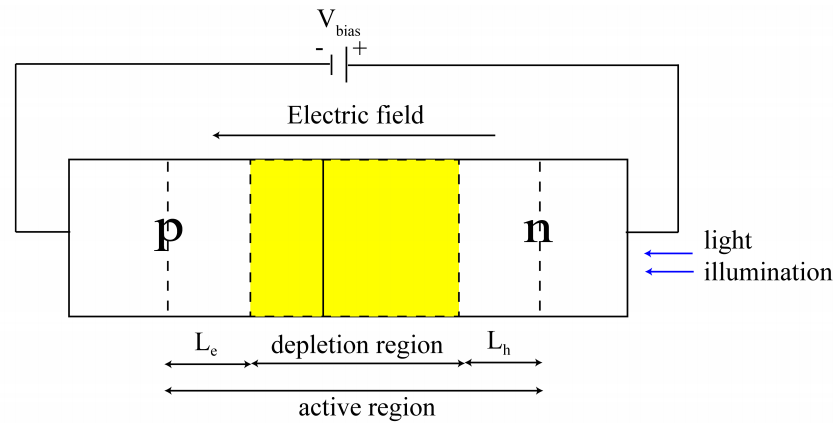
\includegraphics[width=\linewidth,keepaspectratio]{figures/background/photodiode.png}
	\caption{Photodiode schematic. L\textsubscript{e}, L\textsubscript{h} are electron, hole diffusion lengths respectively\cite{Xu2015FundamentalCO}}
	\label{fig:photodiode.png}
\end{figure}
A photodiode is a p-n junction\anote{pnjunction} operated in reverse bias mode\anote{reversebias}.
%
When a photon of sufficient energy is absorbed by the diode, it creates an electron-hole pair.
%
If the creation event happens within the active region then the hole moves out through the p-type material and the electron moves out through the n-type material.
%
This establishes a \textit{photocurrent} that can be read by a reading circuit (see figure ~\ref{fig:3tpixel}).
\begin{figure}
	\center
	
\includegraphics[width=.5\linewidth,keepaspectratio]{figures/background/3t_pixel.png}
	\caption{Three transistor "pixel". M\textsubscript{rst} is the reset transistor (enabling the photodiode to dump charge), M\textsubscript{sf} buffers the charge on the photodiode (so that it can be read without loss), and M\textsubscript{sel} enables a whole row of pixels to be read simultaneously (since all pixels in a physical row are tied to the same row line).}
	\label{fig:3tpixel}
\end{figure}
CMOS sensor arrays do not shift the charge from row to row like CCD arrays.
%
In a CMOS sensor array, each pixel contains a transistor M\textsubscript{sel} controlled by the voltage applied across a row (see figure~\ref{fig:cmosarray}).
%
In order to read one row of pixels, a row line is raised high to turn on (close) all the M\textsubscript{sel} transistors in the row.
%
This brings the signals from all the pixels in that row to the shifter register below by way of the column lines.
%
The shift register then outputs the values of the pixels.
%
The high number of transistors needed per pixel in CMOS arrays has only recenty been manageable for semiconductor foundries.
%
This, along with such artifacts as the "rolling shutter" effect produced by rowline reading, are some of the drawbacks of CMOS arrays relative to CCD arrays.
%
Despite this CMOS arrays have become the most common imaging system in consumer goods such as cell phones and digital cameras due to their relatively simple mechanics.
\begin{figure}
	\center
	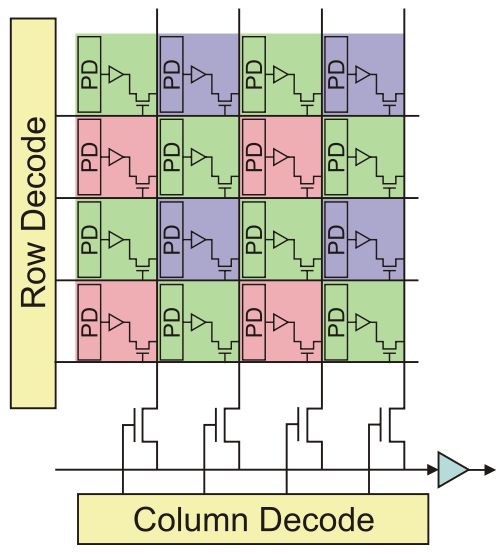
\includegraphics[width=.6\linewidth,keepaspectratio]{figures/background/cmos.png}
	\caption{CMOS array}
	\label{fig:cmosarray}
\end{figure}
\subsubsection{Microbolometers}
Both CCD arrays and CMOS arrays only capture visible light.
%
A microbolometer, on the other hand, measures the power in the infrared by exposing a thermistor\anote{thermistor} to the incident light.
%
\begin{figure}[b]
	\center
	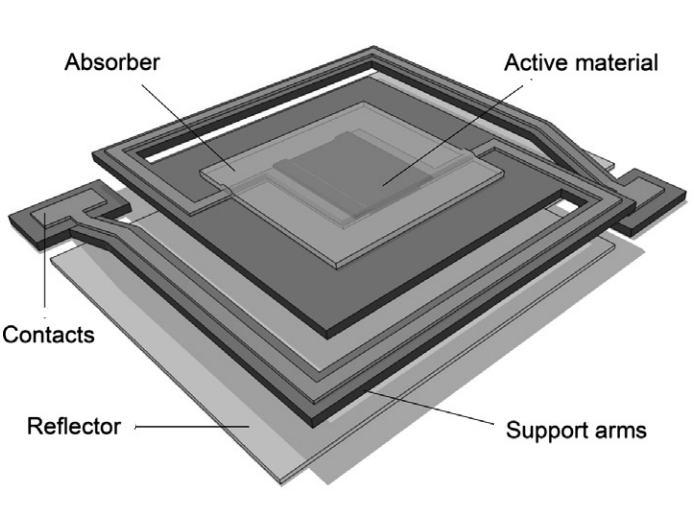
\includegraphics[width=.7\linewidth,keepaspectratio]{figures/background/microbolometer2.png}
	\caption{Bridge structure of Honeywell microbolometer\cite{KESIM2014245}}
	\label{fig:microbolometer}
\end{figure}
%
Since a thermistor's resistance changes as a function of its temperature, a key issue in the design of a microbolometer is the thermal isolation of the thermistor.
%
With the maturation of micro-machining techniques (such as for MEMS\anote{mems} devices) over the last some years, two level microbolometers consisting of a thermo-sensitive component suspended above (and insulated from) silicon have been built (see figure~\ref{fig:microbolometer}).
%
These pixel packages are evacuated and therefore have good conduction, convection, radiation heat transfer properties.
%
The actual thermo-sensitive component consists of a thermistor, an absorber (which aids in transfer of heat to the thermistor), and a reflector that creates a Fabry–Pérot optical cavity\anote{fabryperot} (typically ${\sim}\lambda/4$\cite{bolometer}) that traps the infrared light.
%
Typical materials for the thermistor are vanadium oxide and amorphous silicon owing to their high temperature coefficients of resistance\cite{bolometer}, which in effect transform small changes in temperature into large changes in resistance.
%
Measurements of the thermistor are performed by a read-out integrated circuit adjacent to the bridge in the silicon substrate.
%
All told microbolometers are designed much differently from either CCD or CMOS arrays.
%
It is as a result of this fact that high-resolution infrared cameras are not available.

Across all of these imaging systems there are ample avenues for the introductions of the kinds of errors that degrade image quality and across all of these imaging systems there are structures that impose limitations on resolving power.
%
With that in mind we now proceed to formalizing the problem of super-resolution.

\subsection{Mathematical notation}\label{subsec:notation}
Upper case plain latin $X, Y$ each denote channel $\times$ row $\times$ column \textit{tensors}\anote{tensor} representing LR and HR images respectively, with $(0, 0,0)$ corresponding to the top left corner of the first channel of image.
%
Often for the sake of simplicity we consider greyscale images, in which case we omit the channel dimension.
%
Lower case plain latin $x, y$ denote LR and HR \textit{patches}\anote{patch} respectively.
%
$D, H, F, G$ variously refer to functions that operate on images.
%
Bolded uppercase latin $\bm{X}, \bm{Y}$ are reserved for batches of images, i.e. batch size $\times$ channel $\times$ row $\times$ column tensors with $(0, 0, 0,0)$ corresponding to the top left corner of the first channel of first image in the batch.
%
Bolded lower case denote $\bm{x}, \bm{y}, \bm{z}$ etc. denote conventional column or row vectors.
%
Unless otherwise specified $\left\| \cdot \right\|$ is the $L_2$ norm.

\subsection{Imaging model}\label{subsec:imaging-model}

Figure~\ref{fig:bertrand} shows a conceptual model of the imaging process as carried out by an imaging system.
%
The input to the system is a natural scene that is in effect sampled by the imaging system.
%
In the idealized case the sampling is done at (or above) the Nyquist rate and no aliasing occurs.
%
In practice there is noise and loss introduced at every step of the process: atmospheric turbulence plays a role at large distances, motion produces multiple views of the same scene but also induces blur, imperfections of the lenses further blur the image, and finally down-sampling by the sensor elements into pixels produces aliasing artifacts\anote{ccd}.
%
The noisy, blurry, down-sampled images are then further degraded by sensor noise.
%
Each such image we call an LR sample.
\begin{figure*}
    \centering
    \begin{adjustbox}{width=\textwidth}
        \begin{tikzpicture}[auto]
            \tikzstyle{terminal} = [rectangle, draw, text width=5em, text centered, minimum height=4em]
            \tikzstyle{block} = [rectangle, draw, fill=gray!20, text width=6em, text centered, rounded corners, minimum height=4em]
            \tikzstyle{line} = [draw, -latex']
            \tikzstyle{sum} = [circle, draw]

            \node[inner sep=0pt] (bertrand) {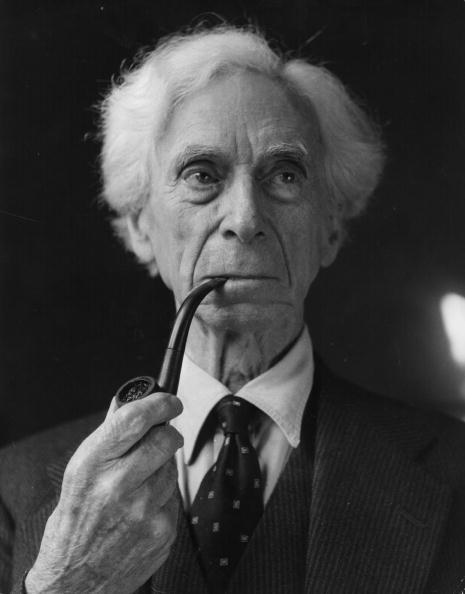
\includegraphics[width=.15\textwidth]{figures/bertrand.png}};
            \node [above = of bertrand] (scene) {Scene};

            \node[sum, right = of bertrand] (sum1) {$+$};
            \node [block, below = of sum1] (atmo-noise) {Atmospheric noise};

            \node [block, right = of sum1] (motion) {Translation, Rotation, Aspect};
            \node [above = of motion] {Motion};

            \node [inner sep=0pt, right = of motion] (motion-output) {};

            \node[inner sep=0pt, below = of motion-output] (bertrand-motion) {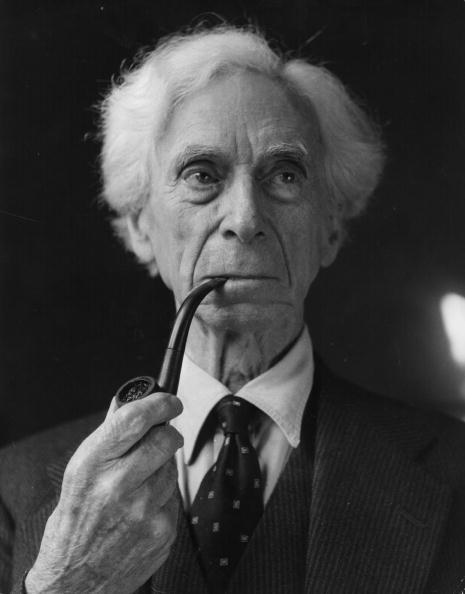
\includegraphics[width=.15\textwidth]{figures/bertrand.png}};
            \node[inner sep=0pt, below = of motion-output, xshift=2mm, yshift=-2mm] {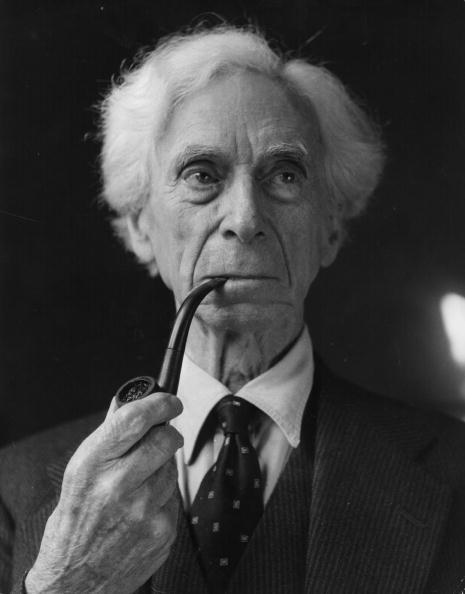
\includegraphics[width=.15\textwidth]{figures/bertrand.png}};
            \node[inner sep=0pt, below = of motion-output, xshift=4mm, yshift=-4mm] {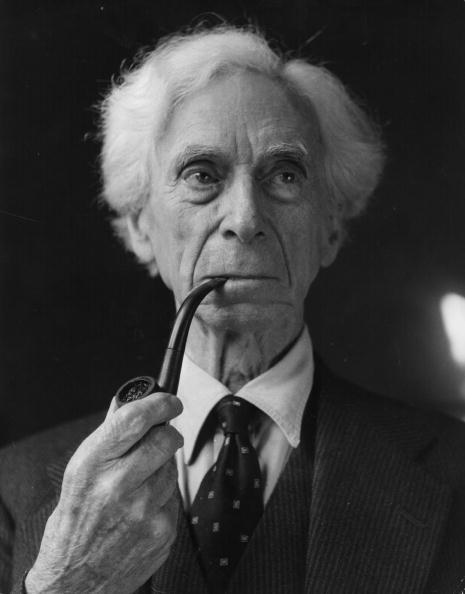
\includegraphics[width=.15\textwidth]{figures/bertrand.png}};
            \node[inner sep=0pt, below = of motion-output, xshift=6mm, yshift=-6mm] {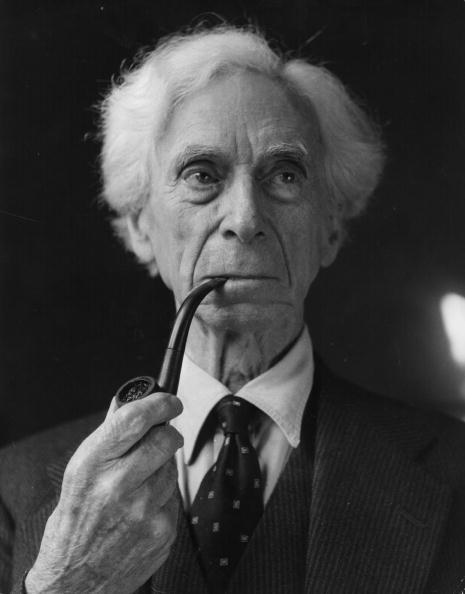
\includegraphics[width=.15\textwidth]{figures/bertrand.png}};

            \node [block, right = of motion-output] (blur) {Optical, Motion};
            \node [above = of blur] {Blur};
            \node [inner sep=0pt, right = of blur] (blur-output) {};

            \node[inner sep=0pt, below = of blur-output] (bertrand-blur) {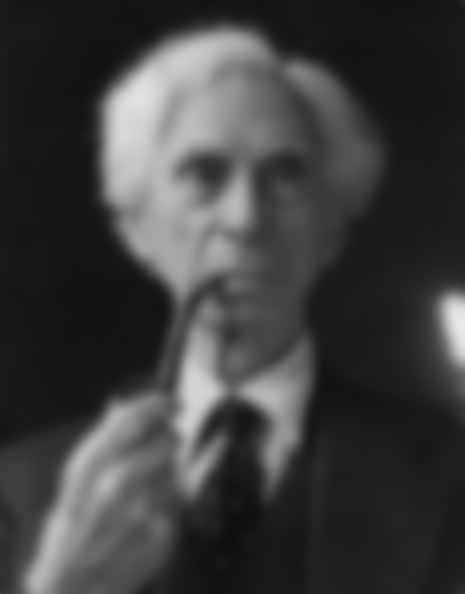
\includegraphics[width=.15\textwidth]{figures/bertrand-blur.png}};
            \node[inner sep=0pt, below = of blur-output, xshift=2mm, yshift=-2mm] {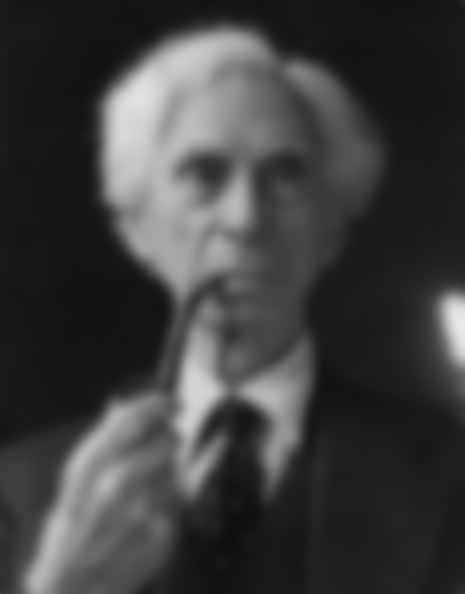
\includegraphics[width=.15\textwidth]{figures/bertrand-blur.png}};
            \node[inner sep=0pt, below = of blur-output, xshift=4mm, yshift=-4mm] {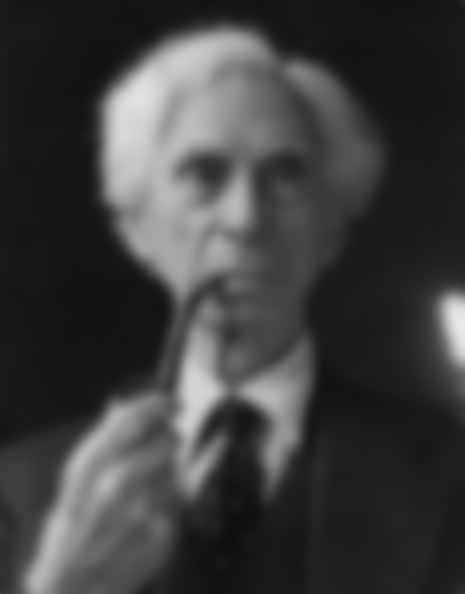
\includegraphics[width=.15\textwidth]{figures/bertrand-blur.png}};
            \node[inner sep=0pt, below = of blur-output, xshift=6mm, yshift=-6mm] {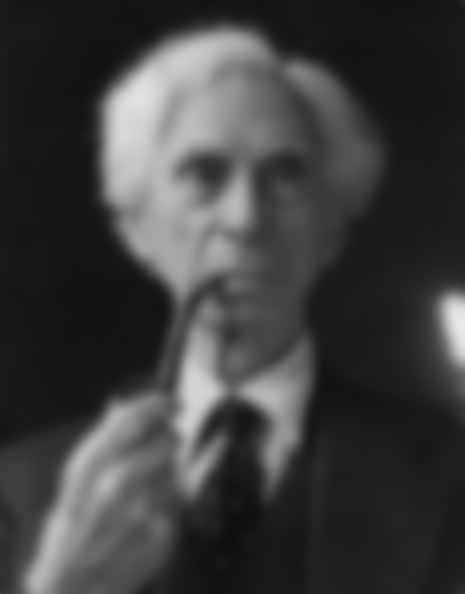
\includegraphics[width=.15\textwidth]{figures/bertrand-blur.png}};

            \node[block, right = of blur-output] (downsample) {Quantization, Pixel-binning};
            \node [above = of downsample] {Down-sampling};

            \node[sum, right = of downsample] (sum2) {$+$};
            \node [block, below = of sum2] (sensor-noise) {Sensor noise};

            \node[inner sep=0pt, right = of sum2] (bertrand-blur-noise) {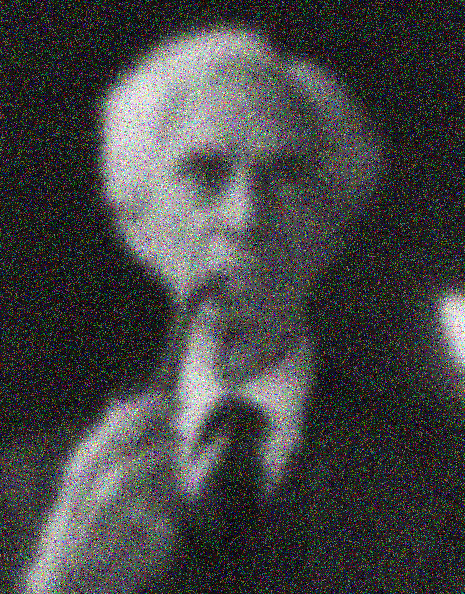
\includegraphics[width=.1\textwidth]{figures/bertrand-blur-noise.png}};
            \node[inner sep=0pt, right = of sum2, xshift=2mm, yshift=-2mm] {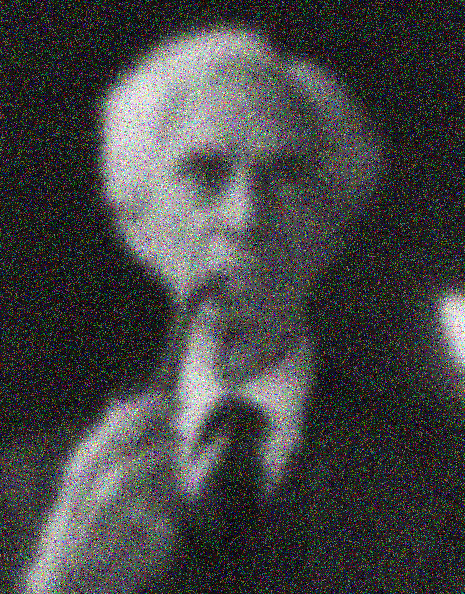
\includegraphics[width=.1\textwidth]{figures/bertrand-blur-noise.png}};
            \node[inner sep=0pt, right = of sum2, xshift=4mm, yshift=-4mm] {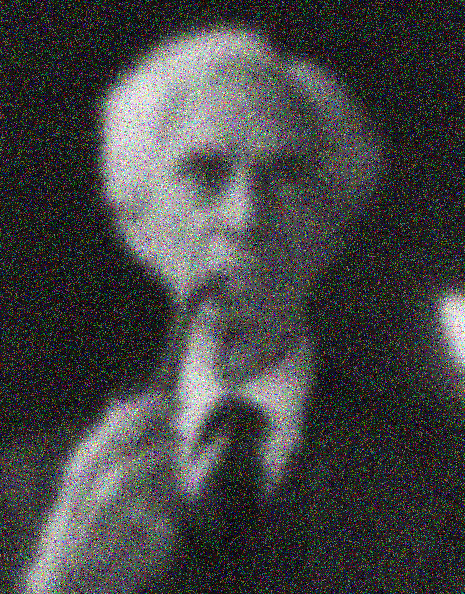
\includegraphics[width=.1\textwidth]{figures/bertrand-blur-noise.png}};
            \node[inner sep=0pt, right = of sum2, xshift=6mm, yshift=-6mm] {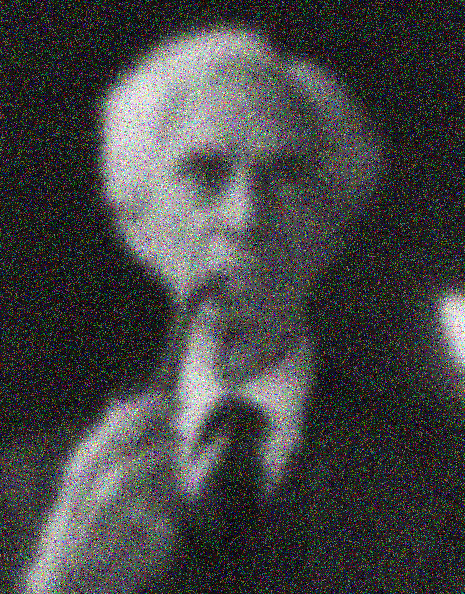
\includegraphics[width=.1\textwidth]{figures/bertrand-blur-noise.png}};
            \node [above = of bertrand-blur-noise, text width=5em] (lr-output) {Low-resolution images};

            \draw[-] (bertrand) edge (sum1);
            \draw[->] (sum1) edge (motion);
            \draw[->] (atmo-noise) edge (sum1);

            \draw[->] (motion) edge (blur);
            \draw[->] (motion-output) edge (bertrand-motion);

            \draw[->] (blur) edge (downsample);
            \draw[->] (blur-output) edge (bertrand-blur);
            \draw[->] (sensor-noise) edge (sum2);
            \draw[-] (downsample) edge (sum2);
            \draw[->] (sum2) edge (bertrand-blur-noise);
        \end{tikzpicture}
    \end{adjustbox}
    \caption{The imaging model illustrating the relationship between a scene and final low-resolution images due to noise, motion, blur, and sampling.}
    \label{fig:bertrand}
\end{figure*}

Let $Y$ denote an idealized HR image of the scene from some fixed vantage point and assume the imaging system collects $K$ LR samples $\Xk$ of $Y$.
%
Formally the $\Xk$ are related to $Y$ by
\begin{equation}
	\Xk = (D \circ H_k \circ A_k) (Y) + \varepsilon_k
	\label{eqn:imagingmodel}
\end{equation}
where for the $k$th LR sample, $A_k$ (of $K$) is the operator representing motion, $H_k$ represents the blur operator, $D$ represents the down-sampling operator (constant in time since it's typically a digital component of the imaging system), and $\varepsilon_k$ represents the composite noise (environment and sensor noise).

\subsubsection{Motion}

In the case of MISR, high-resolution images are constructed by exploiting distinct scene data among multiple low-resolution images.
%
Such distinct data are produced by the relative motion of the imaging system and the scene and therefore precise and accurate image \textit{registration}\anote{registration} is paramount.
%
Successful registration is effected by producing a transformation $f$ that maps pixels at coordinates $(x',y')$ in sample $\Xkone$ to coordinates $(x,y)$ in sample $X_j$
\begin{equation}
	\Xkone(f(x', y')) = X_j(x,y)
	\label{eqn:registration}
\end{equation}
where we use index $j$ to indicate the possibility of registering all samples relative to a fixed reference image (e.g. $j=0$ the first sample) or successive/relative registration (i.e. with $j=k$).
%
While image registration is already challenging in the various domains where samples are treated as canonical, such as remote sensing and medical imaging, in SR it is further complicated by the fact that the images to be registered are assumed uncertain.
%
Therefore, in principle, image registration and super-resolution cannot be decoupled, since image registration accuracy would be improved by operating on the estimated HR images;
%
Hardie \etal~\cite{Hardie1997} use a Bayesian framework to jointly estimate image registration parameters and the high-resolution image\cite{Hardie1997}.
%
Alternatively one can marginalize over the HR image and estimate the registration parameters using maximum-likelihood estimation (MLE) (see section~\ref{subsubsec:gaussianprocess}).

\subsubsection{Blur}

We now consider the challenges and nuances of estimating blur.
%
In general the optical transfer function (OTF) characterizes the blur of an imaging system\anote{otf}.
%
We factor the OTF into three components:
\begin{equation}
	H(u, v) = H_{\text{diff}}(u,v) H_{\text{abr}}(u,v) H_{\text{int}} (u,v)
\end{equation}
where $u,v$ are horizontal and vertical spatial frequencies respectively (measured in cycles/mm), $H_{\text{diff}}$ is blur due to diffraction, $H_{\text{abr}}$ is blur due to lens aberrations, and $H_{\text{int}}$ is blur due to imaging sensor shape (obtained by taking the Fourier transform of the shape an individual sensor in the imaging array).
%
Blur due to diffraction in most imaging systems is due to diffraction through a circular aperture\cite{goodman2005introduction}:
\begin{equation*}
	H_{\text{diff}}(u,v) =   \begin{cases}
		\frac{2}{\pi} \left(\frac{1}{\cos(\tau)} - \tau \sqrt{1-\tau^2}\right) & \text{if } \tau < 0 \\
		0                                                                      & \text{otherwise}
	\end{cases}
\end{equation*}
where $\tau = \rho/\rho_c$, $\rho=\sqrt{u^2 +v^2}$, $\rho_c = 1/\lambda N$ is the radial cutoff frequency of the aperture, $N$ is the f-number\anote{fnumber} of the optics, and $\lambda$ is the wavelength of light being diffracted.
%
This is in fact the filter that produces the Airy pattern and therefore informs sensor array spacing in order to avoid aliasing.
%
Wavelength independent blurring due to aberrations can be induced by various imperfections in the lenses such as spherical aberration, comatic aberration\anote{coma}, or astigmatism. Furthermore, dispersion\anote{dispersion} blurs particular wavelengths of light. A good model for all of these effects is\cite{10.1117.12.946501}:
\begin{equation*}
	H_{\text{abr}}(u,v) =   \begin{cases}
		1-\left(\frac{25}{65}\right)^2 \left(1-4\left(\tau - \frac{1}{2}\right)\right)^2 & \text{if } \tau < 0 \\
		0                                                                                & \text{otherwise}
	\end{cases}
\end{equation*}
Figure~\ref{fig:mtf} shows an example OTF for an imaging system with a sensor spacing of 0.050 mm and therefore sampling frequency of 20 cycles/mm and $\rho_c = 83.3~\text{cycles}/\text{mm}$ ($F=3$ and $\lambda = 4\mu\text{m}$ i.e. near infrared).
%
Notice that $\rho_c$ is much greater than the Nyquist rate ($\frac{1}{2} \times 20~\text{cycles}/\text{mm} = 10~\text{cycles}/\text{mm}$) and therefore many frequencies that are within the radial cutoff frequency will be aliased.
%
This in particular can be mitigated by effectively increasing sampling rate using MISR.
%
Notice also that like a typical transfer function the OTF is not flat and therefore attenuates high spatial frequencies.
%
Simply applying gain to the image wouldn't solve the attenuation problems because of aliasing, but likewise this can be resolved after the effective sampling rate is increased using MISR.
\begin{figure}
	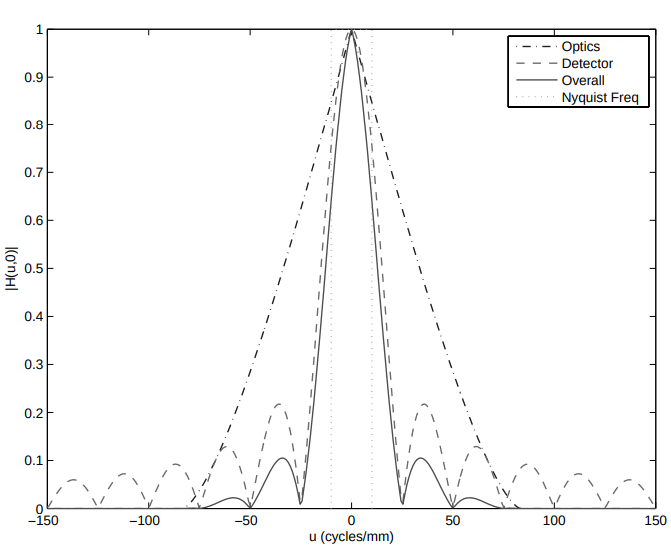
\includegraphics[width=\linewidth,keepaspectratio]{figures/background/mtf.png}
	\caption{OTF magnitude cross-section for\cite{milanfar2017super}}
	\label{fig:mtf}
\end{figure}

The challenge of super-resolution is to solve the inverse problem of finding $Y$ from one or several $\Xk$.
%
In general, since $A_k, H_k, D_k$ are highly degenerate functions, the corresponding inverse problems are ill-posed without regularization and conditioning.
%
The techniques that have been brought to bear on the problem range from interpolation to statistical estimation to example based learning.


\newpage
\begin{figure*}
	\centering
	\begin{adjustbox}{width=\textwidth}
		\begin{tikzpicture}[auto]
			\tikzstyle{diff} = [draw, circle, scale=0.5]
			\foreach \Sigma in {0,...,5} {
					\node[yshift=-350+\Sigma*30, yslant=0.5, xslant=-1.5, scale=1] (bertrand-blur-\Sigma-1) {
						\includegraphics[width=.15\textwidth]{figures/registration/sift/bertrand_sigma_\Sigma.png}
					};
				}
			\foreach \Sigma in {0,...,5} {
					\node[yshift=-160+\Sigma*20, xshift=30, yslant=0.5, xslant=-1.5, scale=0.5] (bertrand-blur-\Sigma-2) {
						\includegraphics[width=.15\textwidth]{figures/registration/sift/bertrand_sigma_\Sigma.png}
					};
				}
			\foreach \Sigma in {0,...,5} {
					\node[yshift=-50+\Sigma*20, yslant=0.5, xshift=30, xslant=-1.5, scale=0.25] (bertrand-blur-\Sigma-3) {
						\includegraphics[width=.15\textwidth]{figures/registration/sift/bertrand_sigma_\Sigma.png}
					};
				}

			\foreach \Sigma in {1,...,5} {
			\begin{scope}[
					yshift=-365+\Sigma*30, xshift=280,every node/.append style={
							yslant=0.5, xslant=-1.5},yslant=0.5, xslant=-1.5
				]
				\node[] (bertrand-dog-\Sigma-1) {
					\includegraphics[width=.15\textwidth]{figures/registration/sift/dog_bertrand_sigma_\Sigma.png}
				};
				\ifnum \Sigma>2
					\foreach \x in {-.8,-.6,-.4}  {
							\foreach \y in {-.8,-.6,-.4} {
									\fill[red!50] (\x,\y) rectangle (\x+.2,\y+.2);
								}
						}
				\fi;

			\end{scope}
			\ifnum \Sigma>2 {
				\draw[yshift=-365+\Sigma*30, step=2mm, xshift=280, black, yslant=0.5, xslant=-1.5] (-1,-1) grid (0,0);
				\draw[yshift=-365+\Sigma*30, xshift=280, black, yslant=0.5, xslant=-1.5] (-1,-1) rectangle (0,0);

				}
			\fi;
			\ifnum \Sigma=4
				\fill[green, yshift=-365+\Sigma*30, xshift=280, yslant=0.5, xslant=-1.5] (-.6,-.6) rectangle (-.4,-.4)
			\fi;
			}
			\foreach \Sigma in {1,...,5} {
					\node[yshift=-365+\Sigma*30, xshift=140, diff] (diff-\Sigma-1){\Large$-$};
				}



			\foreach \Sigma in {1,...,5} {
					\node[yshift=-170+\Sigma*20, xshift=250, yslant=0.5, xslant=-1.5, scale=0.5] (bertrand-dog-\Sigma-2) {
						\includegraphics[width=.15\textwidth]{figures/registration/sift/dog_bertrand_sigma_\Sigma.png}
					};
				}
			\foreach \Sigma in {1,...,5} {
					\node[yshift=-170+\Sigma*20, xshift=140, diff] (diff-\Sigma-2){\Large$-$};
				}



			\foreach \Sigma in {1,...,5} {
					\node[yshift=-45+\Sigma*20, xshift=250, yslant=0.5, xslant=-1.5, scale=0.25] (bertrand-dog-\Sigma-3) {
						\includegraphics[width=.15\textwidth]{figures/registration/sift/dog_bertrand_sigma_\Sigma.png}
					};
				}
			\foreach \Sigma in {1,...,5} {
					\node[yshift=-45+\Sigma*20, xshift=140, diff] (diff-\Sigma-3){\Large$-$};
				}
			%		($(diff-\Sigma-\x) + (0,5mm)$)
			% draw annotations
			\foreach \x in {1,2,3} {
					\foreach \Sigma in {1,...,5} {
							\draw[-] (bertrand-blur-\Sigma-\x) edge (diff-\Sigma-\x);
						}
					\foreach \Sigma in {0,...,4} {
							\pgfmathtruncatemacro{\nodelabel}{1+\Sigma}
							\draw[-] (bertrand-blur-\Sigma-\x) edge (diff-\nodelabel-\x);
						}
					\foreach \Sigma in {1,...,5} {
							\draw[->] (diff-\Sigma-\x) edge (bertrand-dog-\Sigma-\x);
						}
				}
			\coordinate (a) at (-.5, -.5);
			\node (keypoint) [right] at (10,-6) {Candidate Keypoint (not to scale)};
			\tikzstyle{trans} = [thick,->,>=stealth]
			\path[trans] ([] bertrand-blur-3-2.north west) edge[bend left, out=120, in=90] node[above, sloped] {Down-sample 2x} ([] bertrand-blur-0-3.north west);
			\path[trans] ([xshift=2mm] bertrand-blur-3-1.north west) edge[bend left, out=120, in=90] node[above, sloped] {Down-sample 2x} ([] bertrand-blur-0-2.north west);

			\path[trans] ([] keypoint) edge[] node[] {} ([yshift=-365+4*30, xshift=280, yslant=0.5, xslant=-1.5] a);
			\foreach \x in {0,...,4} {
					\pgfmathtruncatemacro{\nodelabel}{\x+1}
					\path[trans] ([xshift=-10mm] bertrand-blur-\x-1.north west) edge[bend left] node[above, sloped] {$k^{\nodelabel}\sigma$} ([xshift=-10mm] bertrand-blur-\nodelabel-1.north west);
				}
		\end{tikzpicture}
	\end{adjustbox}
	\caption{The imaging model illustrating the relationship between a scene and final low-resolution images due to noise, motion, blur, and sampling.}
	\label{fig:bertrand}
\end{figure*}
Images obtained from multiple vantage points, or at different times, of the same scene, become distorted with respect to each other.
%
Since in MISR the aim is to exploit new information across multiple LR samples, we need to first rectify these distortions and reconcile the images.
%
Effectively this means finding one or more pixel transformations that enable mapping all LR images to a common pixel grid.
%
When the transformations cannot be deduced from first principles (e.g., precise knowledge of the relative motion of the scene and the imaging system) they must be estimated from the LR images.
%
The estimation process can be broken down into three distinct steps: feature detection, feature matching, and mapping function estimation.

\subsection{Feature Detection and Selection}\label{sec:featdetec}

Feature detection and selection is the process of identifying features of the image that are presumed to be invariant across the multiple images to be registered.
%
Note that here by features  we mean image artifacts (e.g. edges, contours, line intersections, or corners); in this context encodings or transformations of these image artifacts are called \textit{descriptors}.
%
Features are also known as control points 
%
The CPs are the data that will be used to estimate the transformation \(f\).
%
Therefore, in order that the estimated transformation is accurate, CPs should be robust to noise and image degradation, sufficiently distributed throughout the image, and readily matched in the matching step.

\subsubsection{Harris Corner Detection}
Bentoutou \etal\cite{bentoutou2005automatic} use a Harris detector\cite{harris1988combined} to find corner points, arguing that corners are robust to noise and stable over multiple images.
%
In order to understand the Harris detector we need to first understand the Moravec\cite{moravec1980obstacle} detector on which it improves.
%
The Moravec detector starts from an error function \(E_{x,y}(u,v)\) which computes the sum of the squared differences (SSD) between an \(m \times m\) weighted window around a pixel \(X(x, y)\) and weighted windows shifted by \(u,v\) pixels:
\begin{multline}
	\quad E_{x,y}(u,v) \coloneqq \\ \sum_{i,j=-m/2}^{m/2} w_{ij}\left[ X(x_i+ u,y_j+v) - X(x_i, y_j)\right]^2
	\label{moravecerrorfunction}
\end{multline}
where \(x_i \coloneqq x + i\) and \(y_j \coloneqq y+j\).
\begin{figure}
	\centering
	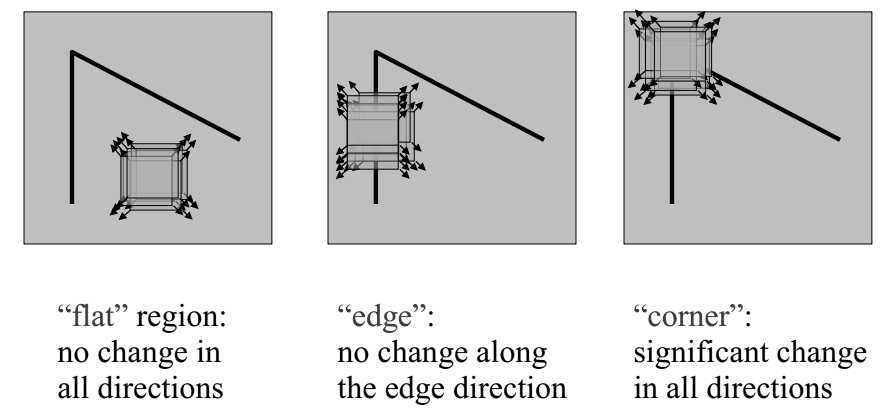
\includegraphics[width=\linewidth,keepaspectratio]{figures/registration/corners.png}
	\caption{Moravec Corner Detector}
	\label{fig:corners}
\end{figure}
Moravec assigns a corner score according to the following reasoning (see figure~\ref{fig:corners}):
\begin{framed}
	\begin{enumerate}
		\item If a pixel is in a region of uniform intensity then \(E_{x,y}(u,v)\) is small for all \(u,v\) (since neighboring windows are similar).
		\item If a pixel is on an edge, then \(E_{x,y}(u,v)\) for either \(u > 0\) or \(v > 0\), but not both, is high.
		\item If a pixel is on a corner, then \(E_{x,y}(u,v)\) for \(u > 0\) and \(v > 0\) is high.
	\end{enumerate}
\end{framed}
The Moravec detector assigns a corner score at pixel coordinate \((x,y)\) equal to \(\min_{u,v} E_{x,y}(u,v)\) in order to select for the third case; high corner scores indicate strong evidence of a corner detection.
%
Moravec comments that this corner score is not isotropic, i.e. if edges aren't aligned with either the pixel axes or diagonals then \(E_{x,y}(u,v)\) will incorrectly be low.
%
Harris' innovation was to linearize \(E_{x,y}(u,v)\) in order to compute a quantity more closely related to the intensity variation in a local neighborhood of a corner pixel:
\begin{equation}
	X(x_i + u,y_j + v) \approx  X(x_i,y_j) + X_u u + X_v v
\end{equation}
where \(X_u \coloneqq \partial X/\partial u\) and similarly \(X_v\) and the partial derivatives are taken at \((x,y)\).
%
This implies
\begin{align}
	E_{x,y}(u,v) & \approx \sum_{i,j=-m/2}^{m/2} w_{ij} \left[X(x_i,y_j) + X_u u + X_v v - X(x_i,y_j)\right]^2                 \\
	             & = \sum_{i,j=-m/2}^{m/2} w_{ij} \left[ X_u^2 u^2 + X_v^2 v^2 + 2 X_u X_v u v\right] \\
	             & = \left[ u,v \right] \begin{bmatrix}
		\sum w_{ij}X_u^2   & \sum w_{ij}X_u X_v \\
		\sum w_{ij}X_u X_v & \sum w_{ij}X_v^2   \\
	\end{bmatrix}  \begin{bmatrix}
		u \\
		v
	\end{bmatrix}          \\
	             & = \left[ u,v \right] M  \begin{bmatrix}
		u \\
		v
	\end{bmatrix} \label{eqn:structurematrix}
\end{align}
%
The matrix in eqn.~\eqref{eqn:structurematrix}, called the \textit{structor tensor} or \textit{second-moment matrix} \(M\), is the quantity Harris investigated.
%
Harris reasoned that the cases of Moravec correspond to conditions on the eigenvalues \(\lambda_1, \lambda_2\) of \(M\):
\begin{framed}
	\begin{enumerate}
		\item If \(\lambda_1 \approx \lambda_2 \approx 0\) then \(X(x,y)\) is in a region of uniform intensity.
		\item If \(\lambda_1 \gg \lambda_2\) or \(\lambda_2 \gg \lambda_1\) then \(X(x,y)\) is on an edge.
		\item \(\lambda_1 \approx \lambda_2 > 0\) then \(X(x,y)\) is on a corner.
	\end{enumerate}
\end{framed}
Notice that if \(w_{ij} = 1\) then this is just the gradient covariance of the image and the Harris detector is essentially a local Principle Components Analysis (PCA).
%
In fact Harris doesn't actually compute the eigenvalues but instead a related quantity called the \textit{strength}:
\begin{align}
	S & \coloneqq \lambda_1 \lambda_2 - \kappa (\lambda_1 + \lambda_2)^2 \\
	  & = \det(M) - \kappa \operatorname{trace}^2(M)
	\label{eqn:strength}
\end{align}
%
To this end (using the Harris detector) Bentoutou \etal~first compute a gradient map of the image using a first order Gaussian filter.
%
They then threshold\anote{threshold} the gradient map at the average gradient value, thereby extracting only sufficiently interesting regions, and compute the strength \(S\) for all pixels.
%
They also apply Non-maximum Suppression\anote{nms} (NMS) using a \(3 \times 3\) window and further threshold the remaining non-zero strength values at a threshold of 1\% of maximum observed strength.
%
Finally only the \(n\) corners with the highest strengths \(S\) are kept.

\subsubsection{SIFT}\label{sec:sift}

\begin{figure}
	\centering
	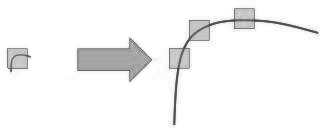
\includegraphics[width=\linewidth,keepaspectratio]{figures/registration/sift/sift_scale_invariant.png}
	\caption{Harris Detector failing to recognize the right image as a corner.}
	\label{fig:sift_harris}
\end{figure}
One issue with Harris detectors is that they're not invariant to scale (see figure~\ref{fig:sift_harris}).
%
Zahra \etal\cite{zahrasift} resolves this issue by using the Scale Invariant Feature Transform\cite{lowe2004distinctive} (SIFT) to identify CPs that, as the name implies, are invariant across multiple scales.
%
SIFT identifies scale invariant and noise robust features of an image, called \textit{keypoints}, by first finding candidate points with high local curvature at multiple scales and then culling according to some heuristics.
\begin{figure*}
	\pgfplotstableread[]{figures/registration/sift/subgrad_hists.csv}\subgradhists;
	\tikzstyle{every picture}+=[remember picture]
	\tikzset{
		pics/greensquare/.style args={#1/#2/#3}{
				code = {
						\draw[green, line width=.5mm] (#1,#2) rectangle (#1+#3, #2+#3);
					}
			},
		subgradbin/.pic={
				\foreach \i in {0.0, 1.0} {
						\pgfmathsetmacro{\x}{0.5+\i*2*.08825};
						\foreach \j in {0.0, 1.0} {
								\pgfmathsetmacro{\y}{0.5+\j*2*.08825};
								\pic[] {greensquare=\x/\y/2*.08825};
							};
					};
			},
		pics/subgradbins/.style args={#1}{
				code = {
						\foreach \x in {0,1,2,3} {
								\pgfmathtruncatemacro{\angle}{#1+\x*90}
								\pic[rotate around={\angle:(0.5,0.5)}] {subgradbin};
							}
					}
			},
		pics/edgehistogram/.style args={#1/#2}{
				code={
						\begin{axis}[area style, width=2.5cm,height=2.5cm, hide axis, at={(#1cm,#2cm)}]
							\addplot+[ybar interval] plot coordinates {
									(-0.50, 2) (0.5, 4) (1.5, 5) (2.5, 3) (3.5, 2) (4.5, 2) (5.5, 0)
								};
							\path
							\foreach[count=\i from 0] \v in {2, 4, 5, 3, 2, 2} {
									(\i, \v) node[below] {\tiny\v}
								};
						\end{axis}
					}
			},
		pics/randomedgehistogram/.style args={#1/#2}{
				code={
						\node (hist-#1#2) at (#1cm+.5cm,#2cm+.5cm) {};% {#1,#2};
						\begin{axis}[area style, width=2.5cm,height=2.5cm, hide axis, at={(#1cm,#2cm)}]
							\pgfmathtruncatemacro{\rowindex}{#1*4+#2}
							\pgfplotstablegetelem{\rowindex}{[index]0}\of{\subgradhists}\pgfmathtruncatemacro{\na}{\pgfplotsretval};
							\pgfplotstablegetelem{\rowindex}{[index]1}\of{\subgradhists}\pgfmathtruncatemacro{\nb}{\pgfplotsretval};
							\pgfplotstablegetelem{\rowindex}{[index]2}\of{\subgradhists}\pgfmathtruncatemacro{\nc}{\pgfplotsretval};
							\pgfplotstablegetelem{\rowindex}{[index]3}\of{\subgradhists}\pgfmathtruncatemacro{\nd}{\pgfplotsretval};
							\pgfplotstablegetelem{\rowindex}{[index]4}\of{\subgradhists}\pgfmathtruncatemacro{\ne}{\pgfplotsretval};
							\pgfplotstablegetelem{\rowindex}{[index]5}\of{\subgradhists}\pgfmathtruncatemacro{\nf}{\pgfplotsretval};
							\pgfplotstablegetelem{\rowindex}{[index]6}\of{\subgradhists}\pgfmathtruncatemacro{\ng}{\pgfplotsretval};
							\pgfplotstablegetelem{\rowindex}{[index]7}\of{\subgradhists}\pgfmathtruncatemacro{\nh}{\pgfplotsretval};
							\addplot+[ybar interval] plot coordinates {
									(-0.50, \na)
									(0.5, \nb)
									(1.5, \nc)
									(2.5, \nd)
									(3.5, \ne)
									(4.5, \nf)
									(5.5, \ng)
									(6.5, \nh)
									(7.5, 0)
								};
							\draw
							\foreach[count=\i from 0] \v in {\na, \nb, \nc, \nd, \ne, \nf, \ng, \nh} {
									(\i, \v) node[below] {\scalebox{.3}{\v}}
								};
						\end{axis}
					}
			},
		array/.style={
				draw,
				minimum width=2em,
				minimum height=2em,
				outer sep=0pt
			},
	}
	\newcommand*{\siftwidth}{.5\linewidth}
	\newcommand*{\length}{sqrt((2.*x^2+2.*y^2)^2 + (8.*x^2*y^2)^2 )}
	\pgfplotsset{
		dominantorientationaxis/.style={
				enlargelimits = false,
				view={0}{90},
				xmin=0, xmax=1, ymin=0, ymax=1,
				ytick distance=1/16,
				xtick distance=1/16,
				axis equal image, grid=both,
				minor grid style={black},
				major grid style={black},
				axis equal image,
			},
	}
	\pgfplotsset{ticks=none}
	\begin{subfigure}{\siftwidth}
		\centering
		\begin{tikzpicture}
			\begin{axis}[dominantorientationaxis]
				\addplot[on layer=axis background] graphics[xmin=0, xmax=1, ymin=0, ymax=1]
					{figures/registration/sift/bert_keypoint.png};
				\addplot[redarrow,quiver={u=\thisrow{u},v=\thisrow{v}}] table {figures/registration/sift/grads.csv};
				\node[dot=5pt](keypoint) at (0.5,0.5) {};
			\end{axis}
			\node (keyp) at (4,6.5) {Keypoint};
			\draw[redarrow] (keyp)--(keypoint);
		\end{tikzpicture}
		\caption{Keypoint neighborhood.} \label{fig:siftdescriptora}
	\end{subfigure}
	\pgfmathsetmacro{\rot}{54}
	\pgfmathsetmacro{\br}{sqrt(2)*.5/2}
	\begin{subfigure}{\siftwidth}
		\centering
		\begin{tikzpicture}
			\begin{axis}[dominantorientationaxis, set layers]
				\addplot[on layer=axis background] graphics[xmin=0, xmax=1, ymin=0, ymax=1]
					{figures/registration/sift/bert_keypoint.png};
				\addplot[redarrow,quiver={u=\thisrow{u},v=\thisrow{v}}] table {figures/registration/sift/grads.csv};
				\node[dot=5pt](keypoint) at (0.5,0.5) {};

				\draw[yellow] (0.5, 0.5) circle [radius=.5];
				\pic[rotate around={\rot:(0.5,0.5)}] {greensquare=.1464/.1464/.707};
				\draw[line width=2pt,red,-latex](.5,.5)--(.5+0.3579, 1);
				\coordinate (gausscircle) at (.75,.25);
				\coordinate (dominantgrad) at (.5+0.25,.5+.35);
				\coordinate (gradsquare) at (.5-\br,.5+\br);
			\end{axis}
			\node (gausswin) at (5,-0.5) {Gradient Window};
			\node (gradwin) at (1,6.5) {Gaussian Window};
			\node (domin) at (4,6.5) {Majority Gradient};
			\draw[redarrow] (gausswin)--(gausscircle);
			\draw[redarrow] (gradwin)--(gradsquare);
			\draw[redarrow] (domin)--(dominantgrad);
		\end{tikzpicture}
		\caption{Oriented and filterd keypoint gradient neigbhorhood.} \label{fig:siftdescriptorb}
	\end{subfigure}
	\vskip\baselineskip
	\begin{subfigure}{\siftwidth}
		\centering
		\begin{tikzpicture}
			\begin{scope}[rotate=\rot,transform shape,local bounding box=scope1]
				\clip[](1.95,1.99) rectangle (6.0,6.03);
				\begin{axis}[dominantorientationaxis, rotate around={-\rot:(.5,.5)}, grid=none]
					\addplot[on layer=axis background] graphics[xmin=0, xmax=1, ymin=0, ymax=1]
						{figures/registration/sift/bert_keypoint.png};
					\addplot[redarrow,quiver={u=\thisrow{u},v=\thisrow{v}}] table {figures/registration/sift/grads.csv};
					\pic[] {subgradbins=\rot};
					\node[dot=5pt](keypoint) at (0.5,0.5) {};
				\end{axis}
			\end{scope}
			\begin{scope}[shift={($(scope1.south)-(0,1cm)$)}]
				\coordinate (gradbin) at (0.5,5.5);
				\node (gradb) at (2,6.5) {Gradient bin};
				\draw[redarrow] (gradb)--(gradbin);
			\end{scope}
		\end{tikzpicture}
		\caption{16 Keypoint neigbhorhood gradient bins.} \label{fig:siftdescriptorc}
	\end{subfigure}
	\begin{subfigure}{\siftwidth}
		\centering
		\begin{tikzpicture}
			\begin{scope}[rotate=\rot,transform shape,local bounding box=scope1]
				\foreach \i [evaluate=\i as \x using \i*1.0] in {0,...,3}{
						\foreach \j [evaluate=\j as \x using \j*1.0] in {0,...,3}{
								\pic {greensquare=\i/\j/1.0};
								\pic {randomedgehistogram=\i/\j};
							}
					}
				\node[dot=5pt](keypoint) at (2.0,2.0) {};
			\end{scope}
			\node (histb) at (2,5.5) {Histogram of gradient orientations};
			\draw[redarrow] (histb)--(hist-32);
			\begin{scope}[shift={($(scope1.south)-(0,1cm)$)}]
				\matrix (A) [matrix of math nodes, nodes={array, anchor=center}, column sep=-\pgflinewidth] {
					\pgfmathtruncatemacro{\rowindex}{3}
					\pgfplotstablegetelem{\rowindex}{[index]0}\of{\subgradhists}\pgfmathprintnumber[fixed,precision=0]{\pgfplotsretval},
					\pgfplotstablegetelem{\rowindex}{[index]1}\of{\subgradhists}\pgfmathprintnumber[fixed,precision=0]{\pgfplotsretval},
					\pgfplotstablegetelem{\rowindex}{[index]2}\of{\subgradhists}\pgfmathprintnumber[fixed,precision=0]{\pgfplotsretval},
					\pgfplotstablegetelem{\rowindex}{[index]3}\of{\subgradhists}\pgfmathprintnumber[fixed,precision=0]{\pgfplotsretval},
					\pgfplotstablegetelem{\rowindex}{[index]4}\of{\subgradhists}\pgfmathprintnumber[fixed,precision=0]{\pgfplotsretval},
					\pgfplotstablegetelem{\rowindex}{[index]5}\of{\subgradhists}\pgfmathprintnumber[fixed,precision=0]{\pgfplotsretval},
					\pgfplotstablegetelem{\rowindex}{[index]6}\of{\subgradhists}\pgfmathprintnumber[fixed,precision=0]{\pgfplotsretval},
					\pgfplotstablegetelem{\rowindex}{[index]7}\of{\subgradhists}\pgfmathprintnumber[fixed,precision=0]{\pgfplotsretval} &
					\pgfmathtruncatemacro{\rowindex}{2}
					\pgfplotstablegetelem{\rowindex}{[index]0}\of{\subgradhists}\pgfmathprintnumber[fixed,precision=0]{\pgfplotsretval},
					\pgfplotstablegetelem{\rowindex}{[index]1}\of{\subgradhists}\pgfmathprintnumber[fixed,precision=0]{\pgfplotsretval},
					\pgfplotstablegetelem{\rowindex}{[index]2}\of{\subgradhists}\pgfmathprintnumber[fixed,precision=0]{\pgfplotsretval},
					\pgfplotstablegetelem{\rowindex}{[index]3}\of{\subgradhists}\pgfmathprintnumber[fixed,precision=0]{\pgfplotsretval},
					\pgfplotstablegetelem{\rowindex}{[index]4}\of{\subgradhists}\pgfmathprintnumber[fixed,precision=0]{\pgfplotsretval},
					\pgfplotstablegetelem{\rowindex}{[index]5}\of{\subgradhists}\pgfmathprintnumber[fixed,precision=0]{\pgfplotsretval},
					\pgfplotstablegetelem{\rowindex}{[index]6}\of{\subgradhists}\pgfmathprintnumber[fixed,precision=0]{\pgfplotsretval},
					\pgfplotstablegetelem{\rowindex}{[index]7}\of{\subgradhists}\pgfmathprintnumber[fixed,precision=0]{\pgfplotsretval} &
					\cdots\cdots\cdots                                                  &
					\pgfmathtruncatemacro{\rowindex}{12}
					\pgfplotstablegetelem{\rowindex}{[index]0}\of{\subgradhists}\pgfmathprintnumber[fixed,precision=0]{\pgfplotsretval},
					\pgfplotstablegetelem{\rowindex}{[index]1}\of{\subgradhists}\pgfmathprintnumber[fixed,precision=0]{\pgfplotsretval},
					\pgfplotstablegetelem{\rowindex}{[index]2}\of{\subgradhists}\pgfmathprintnumber[fixed,precision=0]{\pgfplotsretval},
					\pgfplotstablegetelem{\rowindex}{[index]3}\of{\subgradhists}\pgfmathprintnumber[fixed,precision=0]{\pgfplotsretval},
					\pgfplotstablegetelem{\rowindex}{[index]4}\of{\subgradhists}\pgfmathprintnumber[fixed,precision=0]{\pgfplotsretval},
					\pgfplotstablegetelem{\rowindex}{[index]5}\of{\subgradhists}\pgfmathprintnumber[fixed,precision=0]{\pgfplotsretval},
					\pgfplotstablegetelem{\rowindex}{[index]6}\of{\subgradhists}\pgfmathprintnumber[fixed,precision=0]{\pgfplotsretval},
					\pgfplotstablegetelem{\rowindex}{[index]7}\of{\subgradhists}\pgfmathprintnumber[fixed,precision=0]{\pgfplotsretval}
					\\};
				\draw[decorate,decoration={brace, amplitude=10pt, raise=5pt, mirror}]
				(A-1-1.south west) to node[black,midway,below= 15pt] {$16 \times 8 = 128$ entries} (A-1-4.south east);%
				\draw[redarrow] (hist-03) -- (A-1-1);
				\draw[redarrow] (hist-02) -- (A-1-2);
				\draw[redarrow] (hist-01) -- (A-1-3);
				\draw[redarrow] (hist-00) -- (A-1-3);
				\foreach \i in {1,...,2}{
						\foreach \j in {0,...,3}{
								\draw[redarrow] (hist-\i\j) -- (A-1-3);
							}
					}
				\draw[redarrow] (hist-33) -- (A-1-3);
				\draw[redarrow] (hist-31) -- (A-1-3);
				\draw[redarrow] (hist-32) -- (A-1-3);
				\draw[redarrow] (hist-30) -- (A-1-4);
			\end{scope}
		\end{tikzpicture}
		\caption{Histogram of gradient orientations descriptor.} \label{fig:siftdescriptord}
	\end{subfigure}
	\caption{Sift keypoint descriptor construction.} \label{fig:siftdescriptor}
\end{figure*}


%
It then \textit{describes} these keypoints by a rotation invariant and noise robust representation.
%
The algorithm consists of five steps:
%
\begin{framed}
	\begin{enumerate}
		\item \textbf{Scale-space pyramid construction}: a sequence of increasingly sub-sampled and more strongly Gaussian filtered images is computed. The sequence of differences of these images is also computed; the sequence of differenced images approximates the multi-scale Laplacian of Gaussians\footnotemark (LoG) of the image (see figure~\ref{fig:siftpyramid}).
		\item \textbf{Keypoint detection}: candidate keypoints are points on edges with non-zero curvature, i.e. extrema along scale and space dimensions in the LoG pyramid (see figure~\ref{fig:siftpyramid}).
		\item \textbf{Keypoint selection}: candidate keypoints are more precisely localized using an iterative process. Keypoints of low-contrast (therefore sensitive to noise) or on edges of low curvature\footnotemark are culled.
		\item \textbf{Keypoint orientation assignment}: orientation is assigned to each keypoint by taking a weighted majority vote of all gradient orientations in a neighborhood of the keypoint (see figure~\ref{fig:siftdescriptorb}). Large minority votes (80\% of majority) are used to create more keypoints at the same pixel point.
		\item \textbf{Keypoint descriptor computation}: for each keypoint the descriptor is computed by partitioning the keypoint's neighborhood into \(2^k\) sub-neighborhoods, computing an 8-bin histogram of oriented gradients\footnotemark (HOG) in each sub-neighborhood, and concatenating (see figure~\ref{fig:siftdescriptord}). In Lowe \etal\cite{lowe2004distinctive} \(2^4=16\) sub-neighborhoods are used to produce an \(8\times16 = 128\) entry length descriptor. The descriptor is also normalized to unit length in order to make it invariant to luminance (intensity).
	\end{enumerate}
\end{framed}
\addtocounter{footnote}{-3}
{
	\makeatletter
	\renewcommand\@makefnmark{\hbox{\@textsuperscript{\normalfont\color{white}\@thefnmark}}}
	\renewcommand\@makefntext[1]{%
	  \parindent 1em\noindent
				\hb@xt@1.8em{%
					\hss\@textsuperscript{\normalfont\@thefnmark}}#1}
	\makeatother

\anote{log}
\anote{smallcurvature}
\anote{hog}
}

SIFT is indeed effective as a CP detector but unfortunately it is patented.
%
Alternatives include Binary Robust Invariant Scalable Keypoints\cite{leutenegger2011brisk}, and Oriented FAST and rotated BRIEF\cite{rublee2011orb} (which itself consists of applying Features from Accelerated Segment Test\cite{rosten2006machine} to detect points of interest and Binary Robust Independent Elementary Features\cite{calonder2010brief} to compute descriptors).

\subsection{Feature Matching}

After robust features are identified in the reference image and the displaced images, they need to be matched.
%
For example, in SIFT, where the descriptors are designed to be invariant across images, a \(k\)-d tree\anote{kdtree} can be used to efficiently match keypoint descriptors.
%
Although this often leads to false-positive matches (Zahra \etal~resolve this by using Random Sample Consensus\anote{ransac}) it's a natural feature matching method.
%
In other cases the matching mechanism is not so straightforward; for a class of algorithms called area-based or intensity-based algorithms, that in fact combine the feature detection and matching step into one, matching involves comparing summaries of patches in the reference image and the displaced image.

\subsubsection{Convex Hull Edges}
%
One technique that matches features explicitly is Point Matching Using Convex Hull Edges\cite{Goshtasby1985}.
%
It operates on the principle that the convex hull\anote{convexhull} of a set of points is invariant under translation, rotation, and scaling.
%
Goshtasby \etal~further argue that a noised set of points will most likely have elements deleted or added in its interior and therefore register the boundaries of the respective convex hulls of the to-be-registered image and the reference image (see figure~\ref{fig:convexhulledges}).
%
\begin{figure}[!htbp]
	\begin{subfigure}{\linewidth}
		\centering
        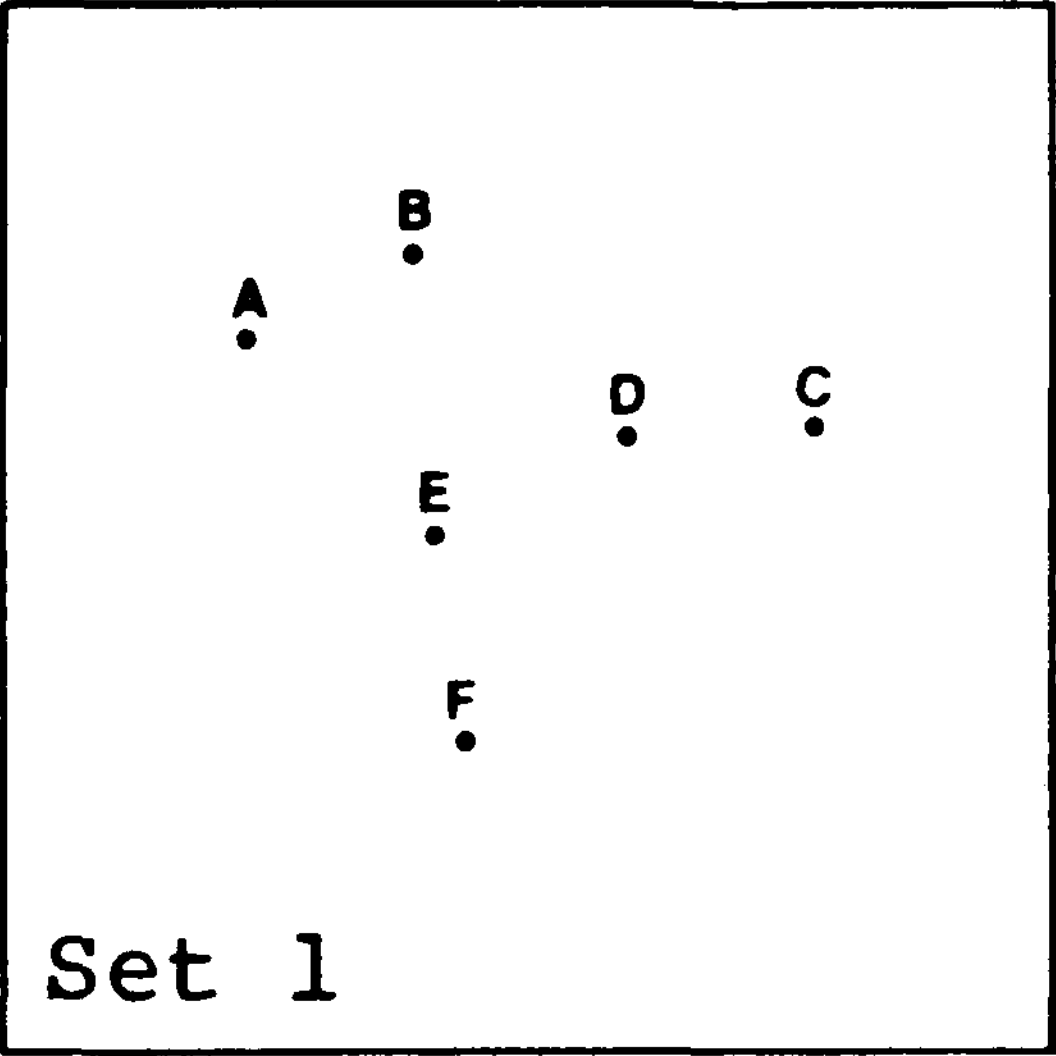
\includegraphics[width=.48\textwidth]{figures/registration/convex/set1.png}
        \raisebox{1px}{
			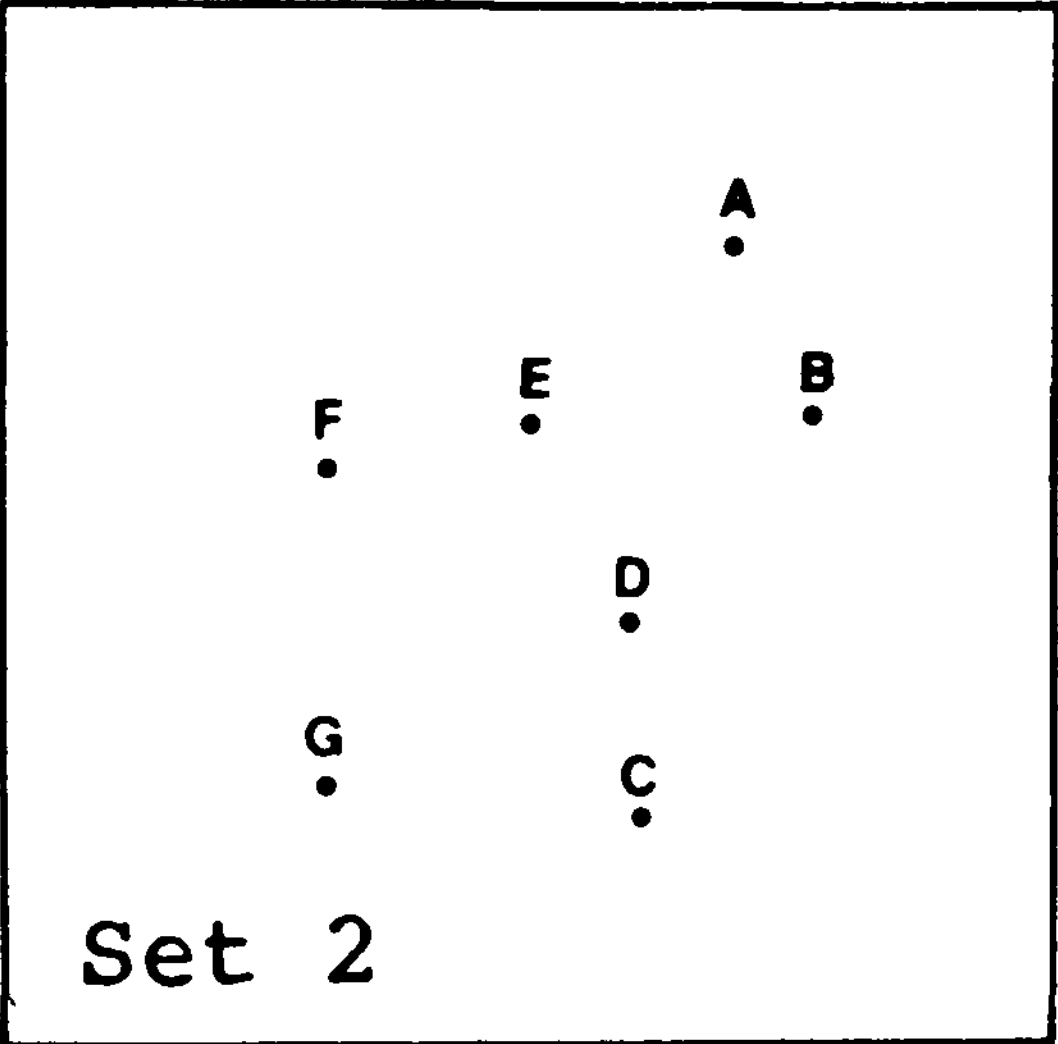
\includegraphics[width=.48\textwidth]{figures/registration/convex/set2.png}
		}
		\caption{Two sets of points. Set 2 is 90 degrees rotated and has extra point \(G\).} \label{fig:twosetsofpoints}
	\end{subfigure}
	\vskip\baselineskip
	\begin{subfigure}{\linewidth}
		\centering
		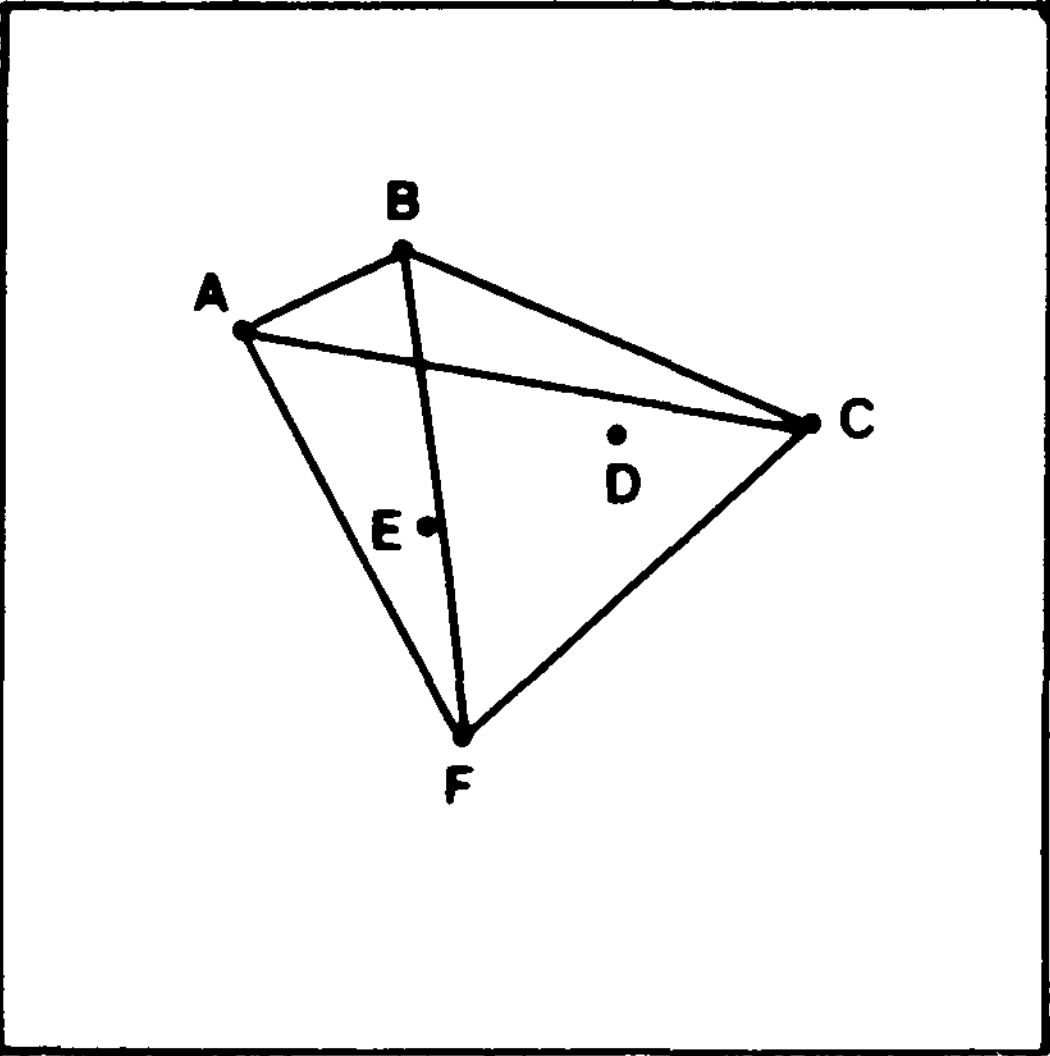
\includegraphics[width=.48\textwidth]{figures/registration/convex/complete_graph_set1.png}
		\raisebox{0.5px}{
			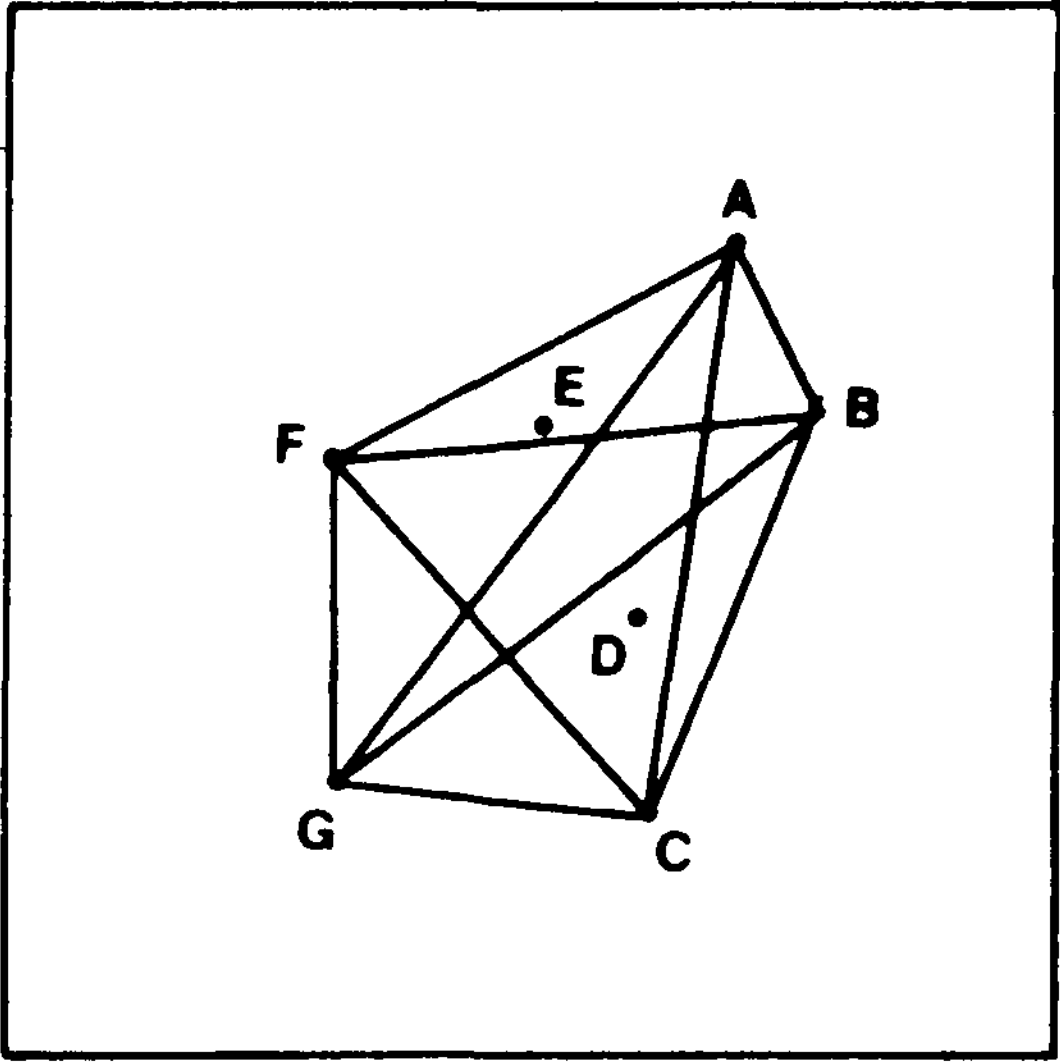
\includegraphics[width=.48\textwidth]{figures/registration/convex/complete_graph_set2.png}
		}
		\caption{Convex hull complete graph edges of two sets, used by the point matching using convex hull edges algorithm.} \label{fig:twoconvexcomplete}
	\end{subfigure}
	\caption{Point matching using convex hull edges \cite{Goshtasby1985}.}
	\label{fig:convexhulledges}
\end{figure}

The key part of the algorithm (after computing the convex hull of the control points) is estimating transformation parameters between convex hull boundaries \(C_1, C_2\):
%
\begin{framed}
	\begin{enumerate}
		\item Determine the complete graphs\footnotemark \(G_1=(V_1, E_1)\), \(G_2 = (V_2,E_2)\) of \(C_1\) and \(C_2\). Then \[\abs{E_1} = \frac{\abs{V_1} (\abs{V_1}-1)}{2}\] (\(\abs{V_1}\) choose 2) and similarly \(\abs{E_2}\). Since there are 2 ways to match any undirected edge we extend \(E_2\) to include reverse directed edges and therefore \[\abs{E_2} = \abs{V_2} (\abs{V_2}-1)\]
		\item For each possible pairing of edges \(e_i, e_j\) in \(E_1, E_2\) compute the rotation \(R_{ij}\), scaling \(S_{ij}\), and translation \(T_{ij}\).
		\item Given the composite transformation \(R_{ij} \circ S_{ij} \circ T_{ij}\) count the number \(N_{ij}\) of other points in \(C_1, C_2\) that also match (within a threshold distance \(D\)).
		\item \(N_{IJ} \coloneqq \max_{i,j} N_{ij}\) and \(R_{IJ}\, \circ S_{IJ}\, \circ\, T_{IJ}\) are the transformation parameters between the control points.
	\end{enumerate}
\end{framed}
\addtocounter{footnote}{-1}
{
	\makeatletter
	\renewcommand\@makefnmark{\hbox{\@textsuperscript{\normalfont\color{white}\@thefnmark}}}
	\renewcommand\@makefntext[1]{%
	  \parindent 1em\noindent
				\hb@xt@1.8em{%
					\hss\@textsuperscript{\normalfont\@thefnmark}}#1}
	\makeatother

\anote{completegraph}
}
%
Note that this procedure operates on one set of control points at a time and that there could be many such matchings computed before final registration between images can be performed.

\subsubsection{Normalized Cross-Correlation}
The simplest strategy for matching by region is to grid-search\anote{gridsearch} the space of possible translational shifts \(\Delta x, \Delta y\) and assess the quality of the registration for a given shift using a similarity metric.
%
One such similarity metric is Normalized Cross-Correlation (NCC); for two image patches \(X_1, X_2\) (with the same width, height)
\begin{multline}
	\operatorname{NCC}(X_1, X_2) \coloneqq \\ \frac{\sum_{x,y} \left(X_1(x,y) - \hat{X}_1\right) \left(X_2(x,y) - \hat{X}_2\right)}{\sqrt{\sum_{x,y} \left(X_1(x,y) - \hat{X}_1\right)^2} \sqrt{ \sum_{x,y} \left(X_2(x,y) - \hat{X}_2\right)^2 }}
\end{multline}
where \(\hat{X}_1, \hat{X}_2\) are mean patch values.

\begin{figure}[!htbp]
	\begin{subfigure}{\linewidth}
		\centering
		\begin{adjustbox}{width=.8\textwidth}
			\begin{tikzpicture}
				\node[inner sep=0pt, xshift=50, yshift=-50] (shiftedcat) {
					{\transparent{.5}
\includegraphics[]
							{figures/registration/cross-correlation/trimmed_cat.jpg}
						}};
				\node[inner sep=0pt, xshift=-50pt, yshift=50pt] (shiftedcat) {
					{\transparent{0.5}
\includegraphics[]
							{figures/registration/cross-correlation/shifted_trimmed_cat.jpg}
						}};
				\draw[red, line width=1mm] (-250pt,-250pt) rectangle (250pt,250pt);
				\node(corrwin) at (0,250pt) {};
				\node[label={[label distance=1cm]:\scalebox{5}{Fixed cross-correlation window}}] (corrw) at (0,600pt) {};
				\draw[redarrow, line width=1mm] (corrw)--(corrwin);
			\end{tikzpicture}
		\end{adjustbox}
		\caption{100 pixel shifted images.} \label{fig:shiftedcat}
	\end{subfigure}
	\vskip\baselineskip
	\begin{subfigure}{\linewidth}
		\centering
		\begin{tikzpicture}
			\begin{axis}
				\addplot3 [surf, mesh/rows=19, mesh/ordering=x varies]
				table[col sep=comma] {figures/registration/cross-correlation/surf.csv};
				\node[above] at (axis cs:-110,-110,224141) {\((-100, -100)\)};
			\end{axis}
		\end{tikzpicture}
		\caption{Cross-correlation for various \(\Delta x, \Delta y\) shifts, with highest correlation at the shift.}
		\label{fig:crosscorr}
	\end{subfigure}
	\vskip\baselineskip
	\begin{subfigure}{\linewidth}
		\centering
		\begin{tikzpicture}
			\begin{axis}
				\addplot3 [surf, mesh/rows=19, mesh/ordering=x varies]
				table[col sep=comma] {figures/registration/cross-correlation/delta_surf.csv};
				\node[above] at (axis cs:-110,-110,1) {\((-100, -100)\)};
			\end{axis}
		\end{tikzpicture}
		\caption{Phase-correlation for various \(\Delta x, \Delta y\) shifts, with single peak at the correct shift.}
		\label{fig:phasecorr}
	\end{subfigure}
	\caption{Cross-correlation feature matching.}
	\label{fig:nccshift}
\end{figure}

%
The NCC image registration technique performs a grid-search over possible shifts and compute the cross-correlation of the shifted images (see figure~\ref{fig:shiftedcat}) (usually over a fixed cross-correlation window rather than the entire image for the sake of computational efficiency).
%
The maximum response as a function \(\Delta x, \Delta y\) is the imputed translation between the images (see figure~\ref{fig:crosscorr}).
%
An alternative but closely related method is \textit{phase correlation}, based on the Fourier shift theorem\anote{fouriershift}  (the value of going to Fourier space is availability of highly optimized algorithms for computing the Fourier transform).
%
Let \(\mathcal{X}_1(u,v) \coloneqq \mathcal{F}\{X_1(x,y)\}, \; \mathcal{X}_2(u,v) \coloneqq \mathcal{F}\{X_2(x,y)\}\) be the Fourier transforms of the images.
%
Then
\[
	\mathcal{X}_1 = \mathcal{X}_2  e^{-2 \pi i \left(\frac{u \Delta x}{M} + \frac{v \Delta y}{N}\right)}
\]
where \(N,M\) are the dimensions of the images.
%
Define \textit{normalized cross-power spectrum}:
\begin{align}
	R(u,v) & \coloneqq \frac{\mathcal{X}_1\odot \mathcal{X}_2^{*}}{\abs{\mathcal{X}_1 }\abs{\mathcal{X}_2^{*} }}                                                                                                                    \\
	       & = \frac{\mathcal{X}_1\odot \mathcal{X}_1^{*} \, e^{2 \pi i \left(\frac{u \Delta x}{M} + \frac{v \Delta y}{N}\right)}}{\abs{\mathcal{X}_1 }\abs{\mathcal{X}_1^{*} \, e^{-2 \pi i \left(\frac{u \Delta x}{M} + \frac{v \Delta y}{N}\right)} }} \\
	       & = \frac{\mathcal{X}_1\odot \mathcal{X}_1^{*} \, e^{2 \pi i \left(\frac{u \Delta x}{M} + \frac{v \Delta y}{N}\right)}}{\abs{\mathcal{X}_1 }\abs{\mathcal{X}_1^{*} }}                                                               \\
	       & = e^{2 \pi i \left(\frac{u \Delta x}{M} + \frac{v \Delta y}{N}\right)} \label{eqn:singleexp}
\end{align}
where \(\odot\) is Hadamard product\anote{hadamard}, \(\abs{\mathcal{X}_1}\) is the magnitude of \(\mathcal{X}_1\), \(\mathcal{X}_1^*\) is the complex conjugate of \(\mathcal{X}_1\), and we've used the fact that \(\abs{e^{iz}}=1\) for all \(z\).
%
Then the inverse Fourier transform of eqn.~\eqref{eqn:singleexp}
\[
	\mathcal{F}^{-1}\left\{ R(u,v) \right\} = r(x,y) = \delta(x + \Delta x, y + \Delta y)
\]
is a single peak (see figure~\ref{fig:phasecorr}) at \((\Delta x, \Delta y)\).
%
The simplest implementation of NCC only identifies translations but it can be extended to affine transforms\cite{berthilsson1998}.

\subsubsection{Mutual Information}

In general NCC fails for noisy images (i.e., the to-be-registered image is much noisier than the reference image).
%
Mutual information (MI) methods have been successfully employed in such cases; MI is also robust to changes in light intensity, pixel color, and can fit large displacement transformations.
%
The mutual information of two random variables \(X_1, X_2\) is defined
\[
	I (X_1,X_2) \coloneqq H (X_1)+H (X_2)-H (X_1,X_2)
\]
where \(H\) is Shannon-entropy\anote{shannon}.
%
In this context \(X_1\) is the reference image and \(X_2\) is the to-be-registered image.
%
The central challenge in computing MI is in estimating joint \(H(X_1,X_2)\) and marginal \(H(X_1)\) entropies (which are functions of the joint \(P(X_1,X_2)\) and marginal \(P(X_1)\) probabilities).
%
In practice this is done using either Kernel Density Estimation\anote{kde} (KDE) or the joint histogram (i.e. number of common pixel values at same pixel coordinates normalized by total number of pixels).
%
Searching for the registration parameters \(\theta\) that maximize \(I_{\theta} \coloneqq I(X_1,X_2(\theta))\) exhaustively is generally costly (especially if more than just translation parameters are required).
%
Ritter \etal\cite{ritter1999} use simulated annealing to efficiently search the space of all possible parameters.
%
Simulated annealing iterates on the current candidate minimum \(I_{\theta}\) by jumping to potentially new minima in a way that prioritizes near jumps but allows for the possibility of far jumps.
%
They use the Cauchy distribution as the jump proposal function:
\[
	G_k(d) = \frac{t_k}{\pi \left( d^2 + t_k^2 \right)}
\]
where \(t_k\) is a parameter that over time encourages near jumps more and more strongly (called the \textit{temperature}), and \(d\) is the parameter jump distance.
%
To allow escape from local minima of \(I_{\theta}\) it is necessary to occasionally make a jump from the current parameter estimate \(\theta_k\) to a proposed value \(\theta_{k+1}\) that is worse (i.e., for which \(I(\theta_{k+1}) < I(\theta_{k}) \)).
%
This is accomplished by accepting or rejecting the proposed jump with probability determined by an \textit{acceptance function} \(A_k\):
\[
	A_k(\theta_{k}, \theta_{k+1}) \coloneqq \begin{cases}
		1                                                  & \text{if } I(\theta_{k+1}) \geq I(\theta_{k}) \\
		\frac{1}{C t_k}e^{I(\theta_{k}) - I(\theta_{k+1})} & \text{otherwise}
	\end{cases}
\]

\subsection{Transform Estimation}
\begin{figure}
	\begin{subfigure}{\linewidth}
		\centering
		\begin{tabular}{>{\centering}p{3cm}c}
			\(
			\begin{bmatrix}
				\cos(\theta) & -\sin(\theta) & t_x \\
				\sin(\theta) & \cos(\theta)  & t_y \\
				0            & 0             & 1   \\
			\end{bmatrix}
			\)
			 &
			\(
			\vcenter{
				\hbox{
					
\includegraphics[height=.5\linewidth,width=.5\linewidth]{figures/registration/transforms/similarity.png}
				}
			}
			\)
		\end{tabular}
		\caption{Rigid transformation (isometry)} \label{fig:rigidtransformation}
	\end{subfigure}
	\begin{subfigure}{\linewidth}
		\centering
		\begin{tabular}{>{\centering}p{3cm}c}
			\(
			\begin{bmatrix}
				a & b & t_x \\
				c & d & t_y \\
				0 & 0 & 1   \\
			\end{bmatrix}
			\)
			 &
			\(
			\vcenter{
				\hbox{
					
\includegraphics[height=.5\linewidth,width=.5\linewidth]{figures/registration/transforms/affine.png}
				}
			}
			\)
		\end{tabular}
		\caption{Affine transformation} \label{fig:affinetransformation}
	\end{subfigure}
	\begin{subfigure}{\linewidth}
		\centering
		\begin{tabular}{>{\centering}p{3cm}c}
			\(
			\begin{bmatrix}
				a & b & c \\
				d & e & f \\
				g & h & i \\
			\end{bmatrix}
			\)
			 &
			\(
			\vcenter{
				\hbox{
					
\includegraphics[height=.5\linewidth,width=.5\linewidth]{figures/registration/transforms/projective.png}
				}
			}
			\)
		\end{tabular}
		\caption{Projective (perspective) transformation (homography)} \label{fig:projectivetransformation}
	\end{subfigure}
	\begin{subfigure}{\linewidth}
		\centering
		\begin{tabular}{>{\centering}p{4cm}c}
			\(
			\begin{bmatrix}
				a(x,y) & b(x,y) & c(x,y) \\
				d(x,y) & e(x,y) & f(x,y) \\
				g(x,y) & h(x,y) & i(x,y) \\
			\end{bmatrix}
			\)
			 &
			\(
			\vcenter{
				\hbox{
					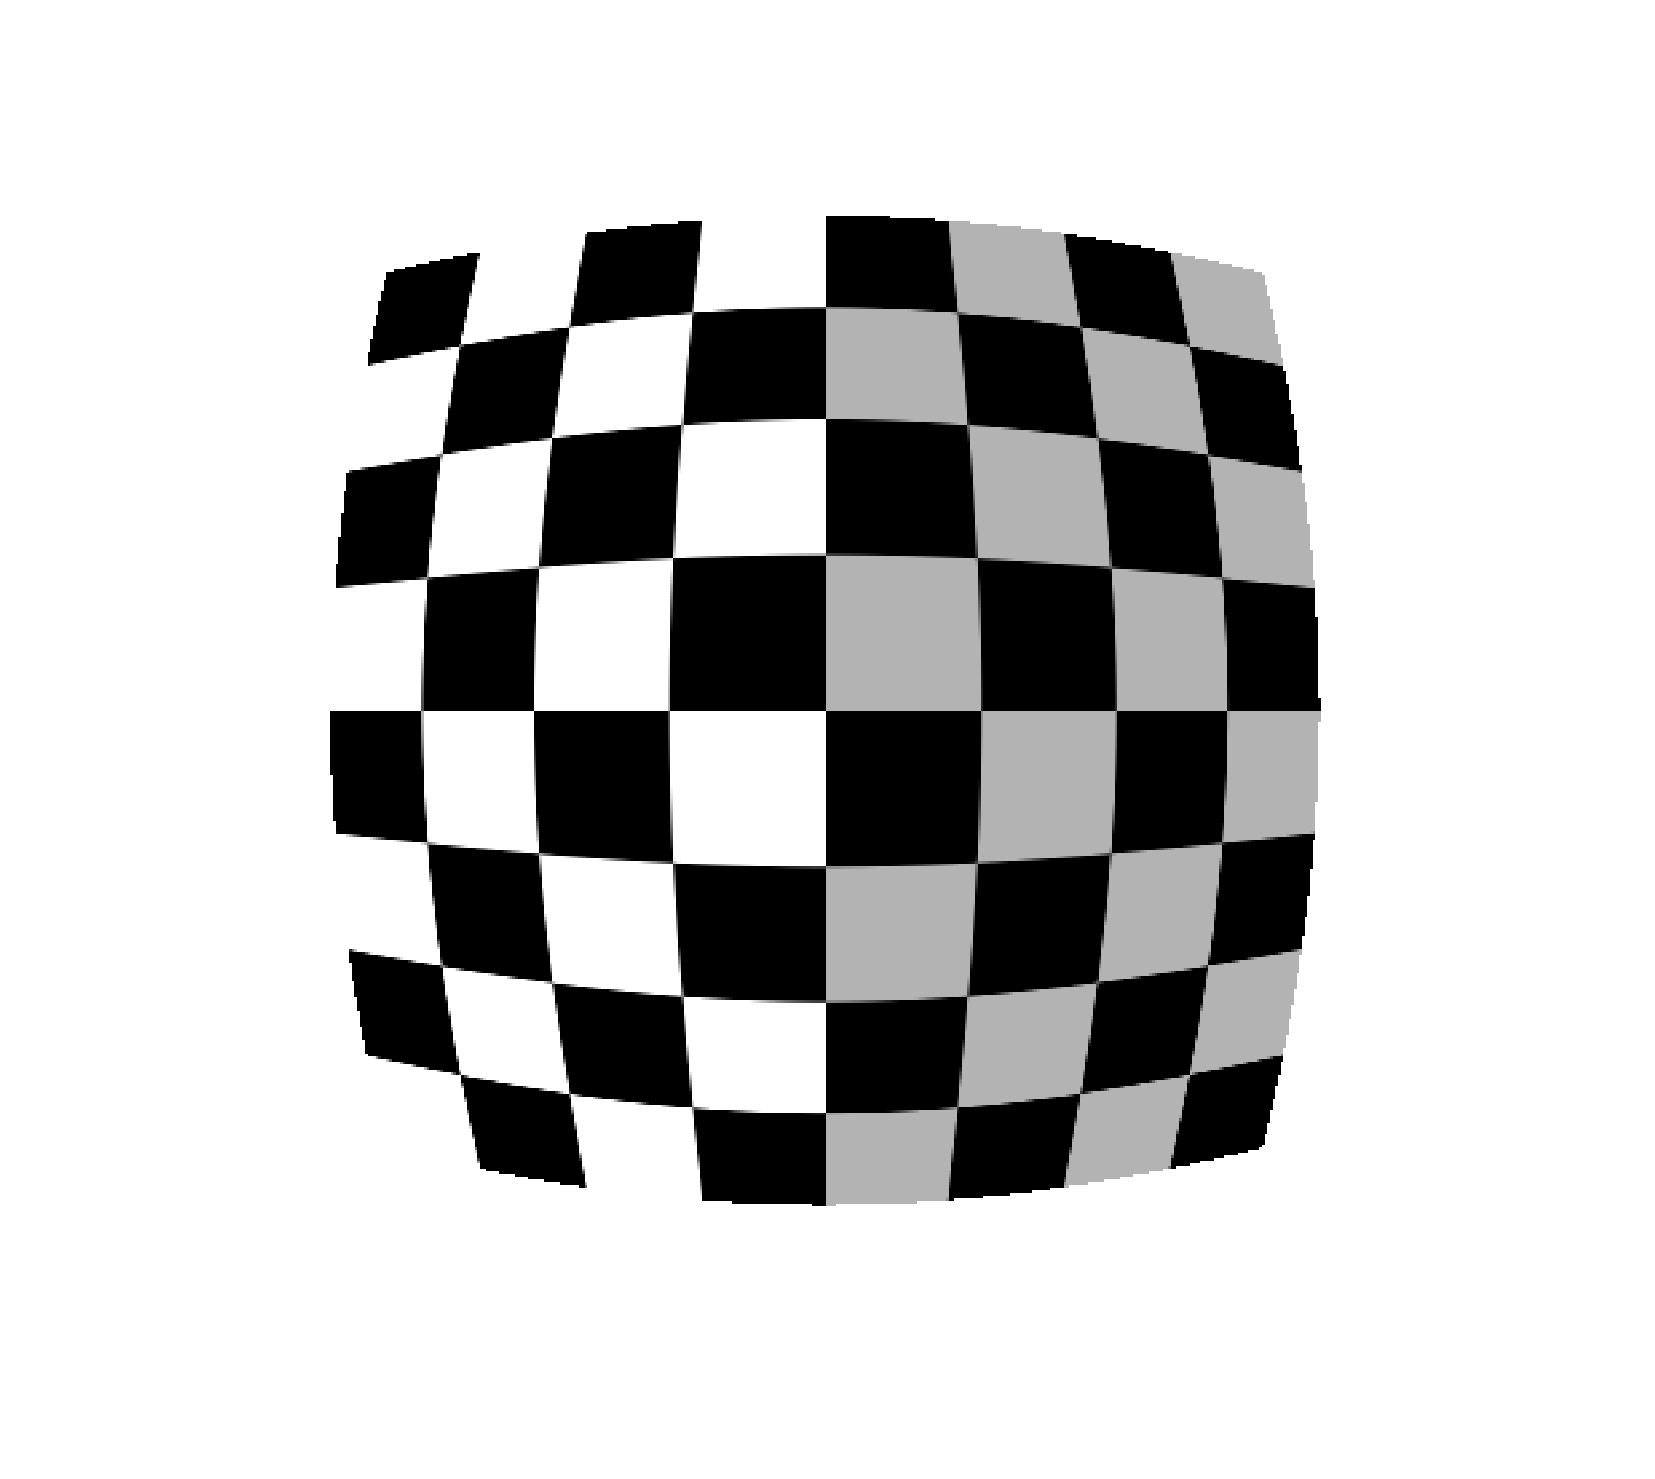
\includegraphics[height=.5\linewidth,width=.5\linewidth]{figures/registration/transforms/barrel.png}
				}
			}
			\)
		\end{tabular}
		\caption{Elastic transformation} \label{fig:elastictransformation}
	\end{subfigure}
	\caption[Compact Routing Example]{Different transformation classes (in homogeneous coordinates) along with realized examples.}
	\label{fig:transformations}
\end{figure}

After feature matching is sucessfully completed the transformation function \(f\) is constructed (see eqn.~\eqref{eqn:registration}).
%
This consists of choosing a transformation type (see figure~\ref{fig:transformations}) and estimating the parameters necessary to uniquely determine the transformation.
%
The transformation type is partially informed by knowledge of the geometry of the displacements (rigid, affine, projective) and partially informed by computational efficiency (more general transformation have more parameters).
%
There are broadly two perspectives on constructing the transformation \(f\): the global perspective which aims to model motion as a map of the image as a whole and the local perspective which aims to model motion as a deformation of individual pixels.
%
%These two perspectives naturally correspond to a globally (see figures~\ref{fig:rigidtransformation}, ~\ref{fig:affinetransformation}, ~\ref{fig:projectivetransformation}) or locally defined transformation \(f\) (see figure~\ref{fig:elastictransformation}).
%
We first quickly cover global algorithms and then move on to more powerful, and more interesting, local algorithms.

\subsubsection{Global Algorithms}

The most commonly used global model is the rigid transformation (see figures~\ref{fig:rigidtransformation}), which in homogeneous coordinates\anote{homogeneous} is defined:
\begin{equation}
	\begin{bmatrix}
		x' \\
		y' \\
		1  \\
	\end{bmatrix} =
	\begin{bmatrix}
		\cos(\theta) & -\sin(\theta) & t_x \\
		\sin(\theta) & \cos(\theta)  & t_y \\
		0            & 0             & 1   \\
	\end{bmatrix}
	\begin{bmatrix}
		x \\
		y \\
		1 \\
	\end{bmatrix}
	\label{eqn:rigidparams}
\end{equation}
The unknown parameters \((\theta, t_x, t_y)\) in eqn.~\eqref{eqn:rigidparams} can be estimated by expanding \(x', y'\) to using Taylor series
\begin{equation}
	\begin{split}
		x' &= t_x + x\left( 1 - \frac{\theta^2}{2} \right) - y\theta  + O(\theta^3) \\
		y' &= t_y + x \theta  + y\left( 1 - \frac{\theta^2}{2} \right) + O(\theta^3)
	\end{split}
	\label{eqn:rigidtaylor}
\end{equation}
Note that this is only valid for small angles \(\theta\) (the small-angle approximation\cite{keren1988}).
%
Truncating eqns.~\eqref{eqn:rigidtaylor} to first or second order and substituting data from matched features yields a system of linear equations.
%
Given that often there are many more matched features than unknowns in eqns.~\eqref{eqn:rigidtaylor} such a system is overdetermined; a unique solution can be determined using regularized least-squares.
%
In order to make this process more efficient and increase accuracy Keren \etal\cite{keren1988} use a Gaussian pyramid (see figure~\ref{fig:siftpyramid} and corresponding discussion in section~\ref{sec:sift}) to iteratively refine estimates at higher and higher resolutions.
%
In the more general case of a projective transformation (a perspective shift) the transformed pixel coordinates are
\begin{equation}
	\begin{split}
		x' & = \frac{ax+by+c}{gx+hy+i} \\
		y' & = \frac{dx+ey+f}{gx+hy+i}
		\label{eqn:projectivetf}
	\end{split}
\end{equation}
and similarly the unknowns (\(a,b,\dots, i\)) can be estimated from matched feature correspondence data.

\subsubsection{Local Algorithms}
\paragraph{Optical Flow}
\begin{figure}[!htbp]
	\begin{subfigure}{\linewidth}
		\centering
		\begin{adjustbox}{height=.7\textwidth}
			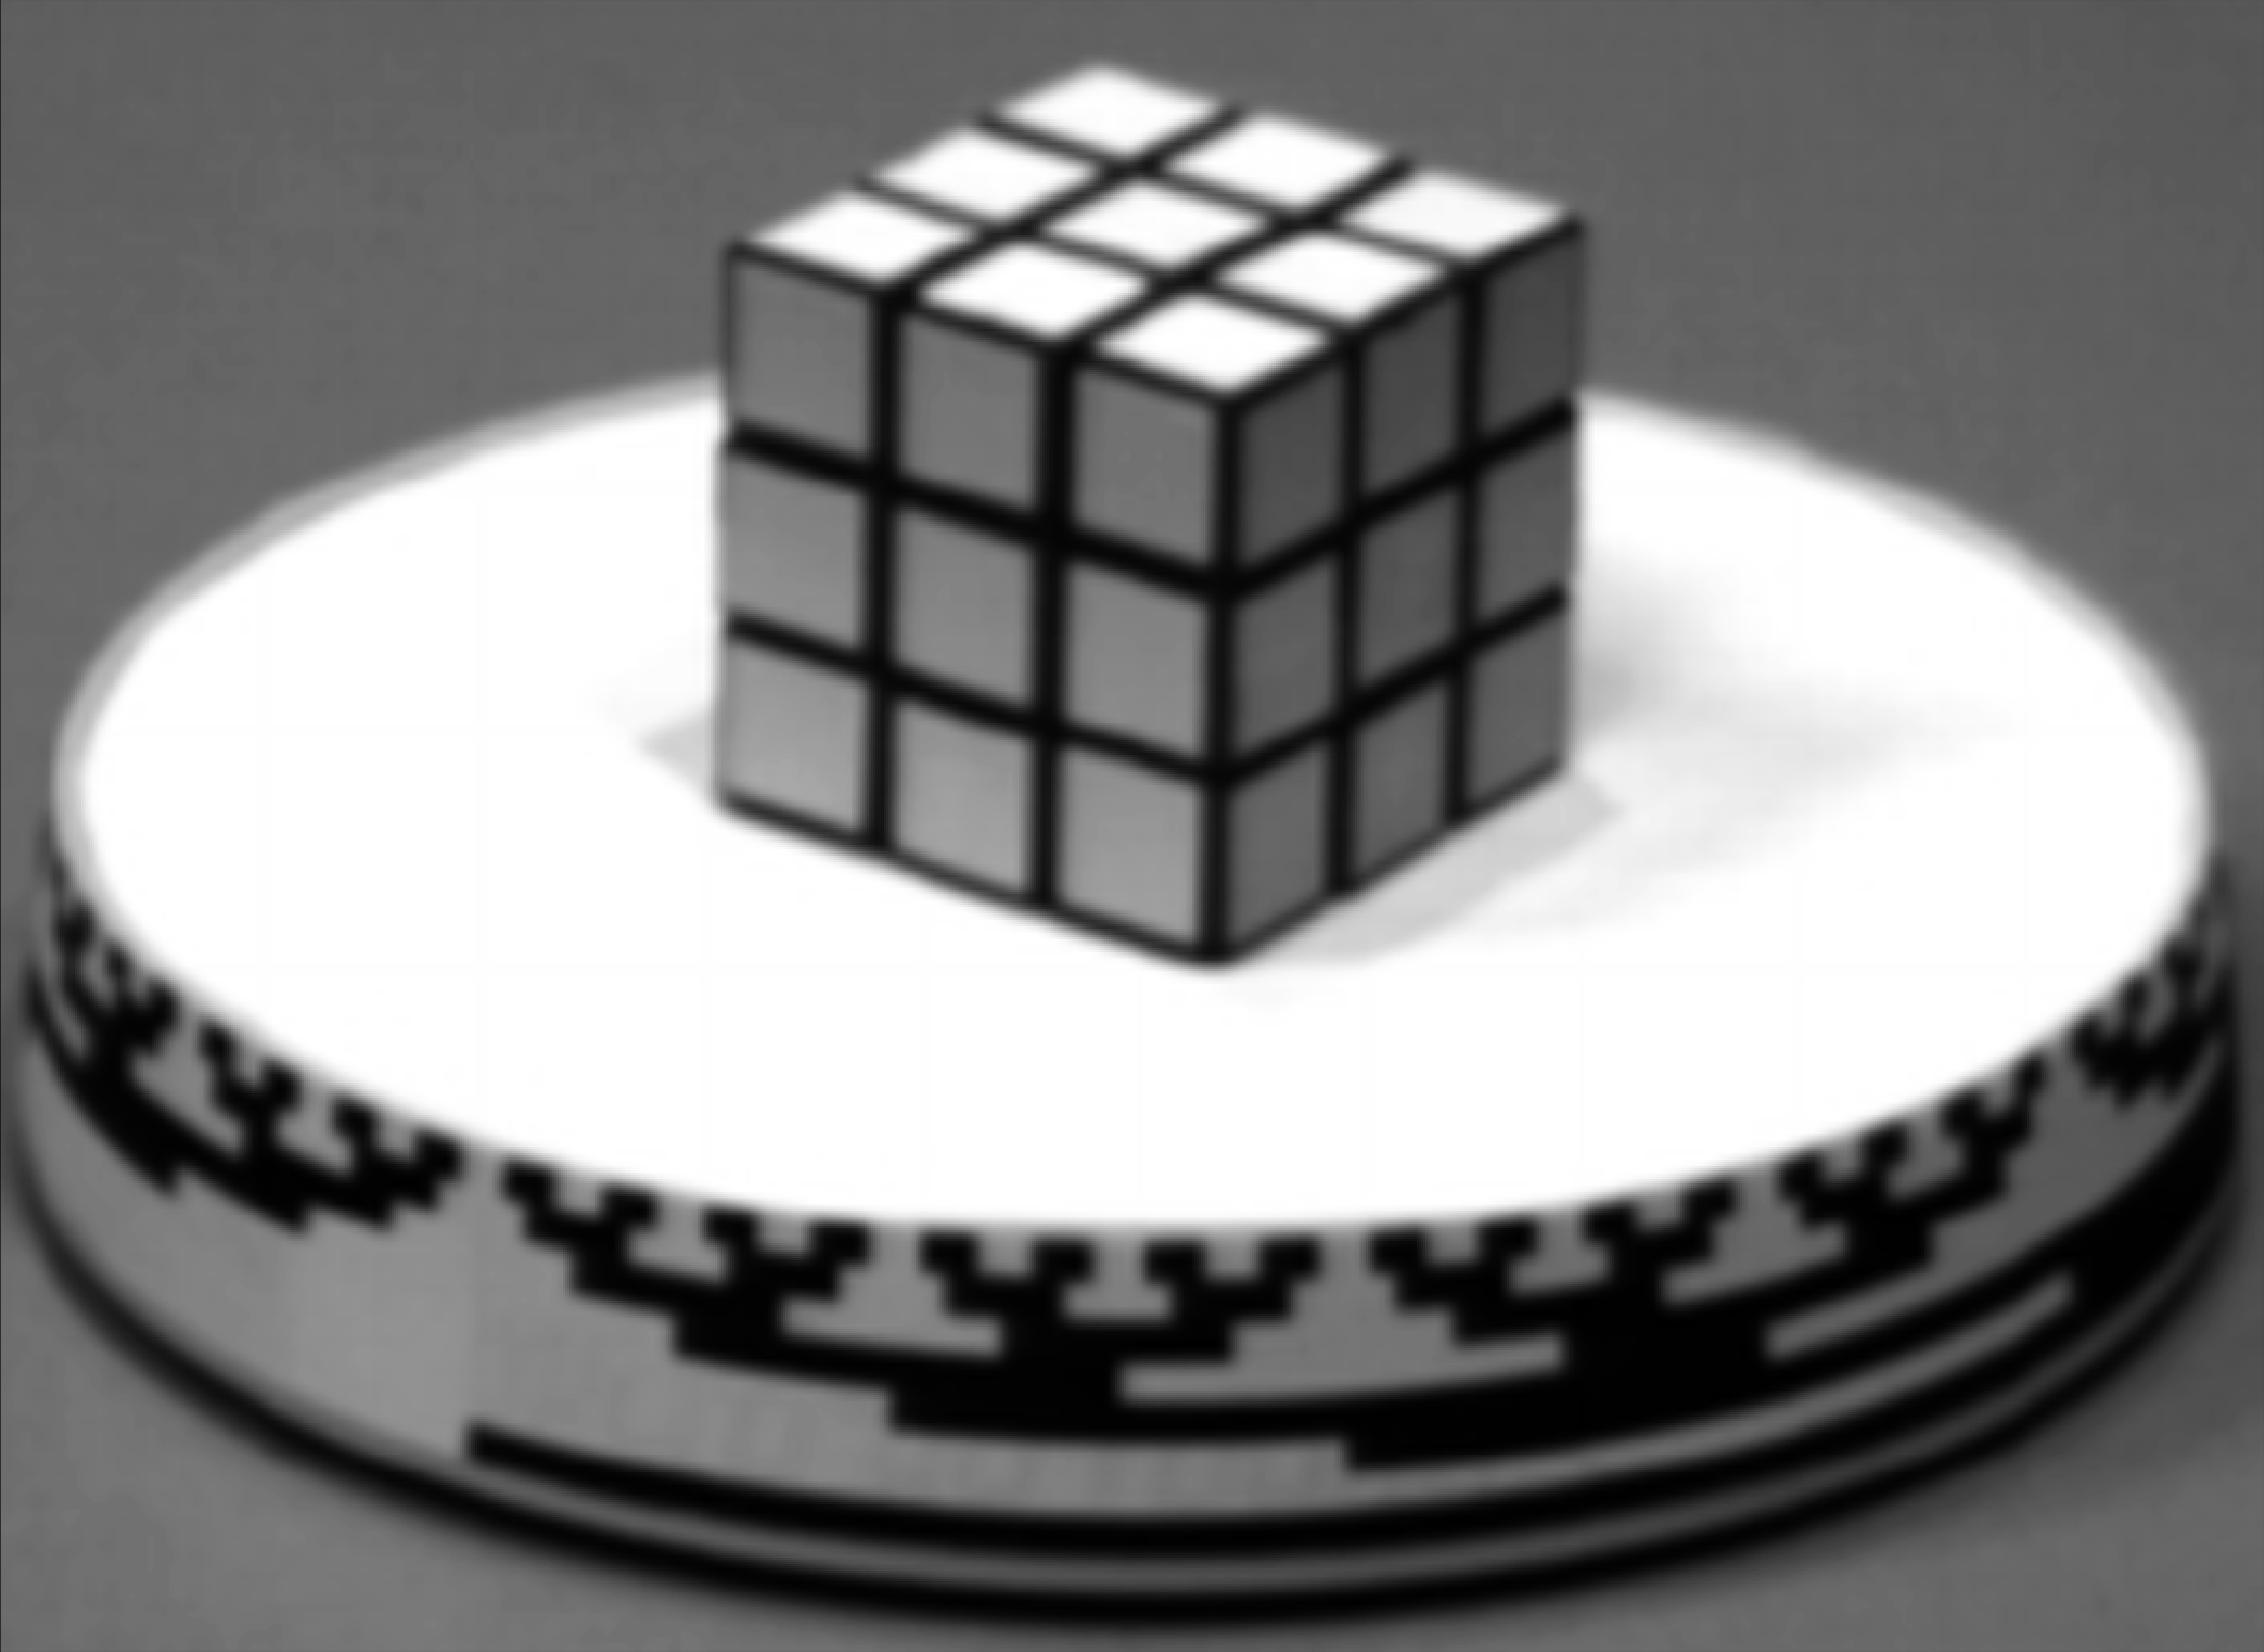
\includegraphics[]
			{figures/registration/optical_flow/reference_image.png}
		\end{adjustbox}
		\caption{Reference image.} \label{fig:refoptical}
	\end{subfigure}
	\vskip\baselineskip
	\begin{subfigure}{\linewidth}
		\centering
		\begin{adjustbox}{height=.7\textwidth}
			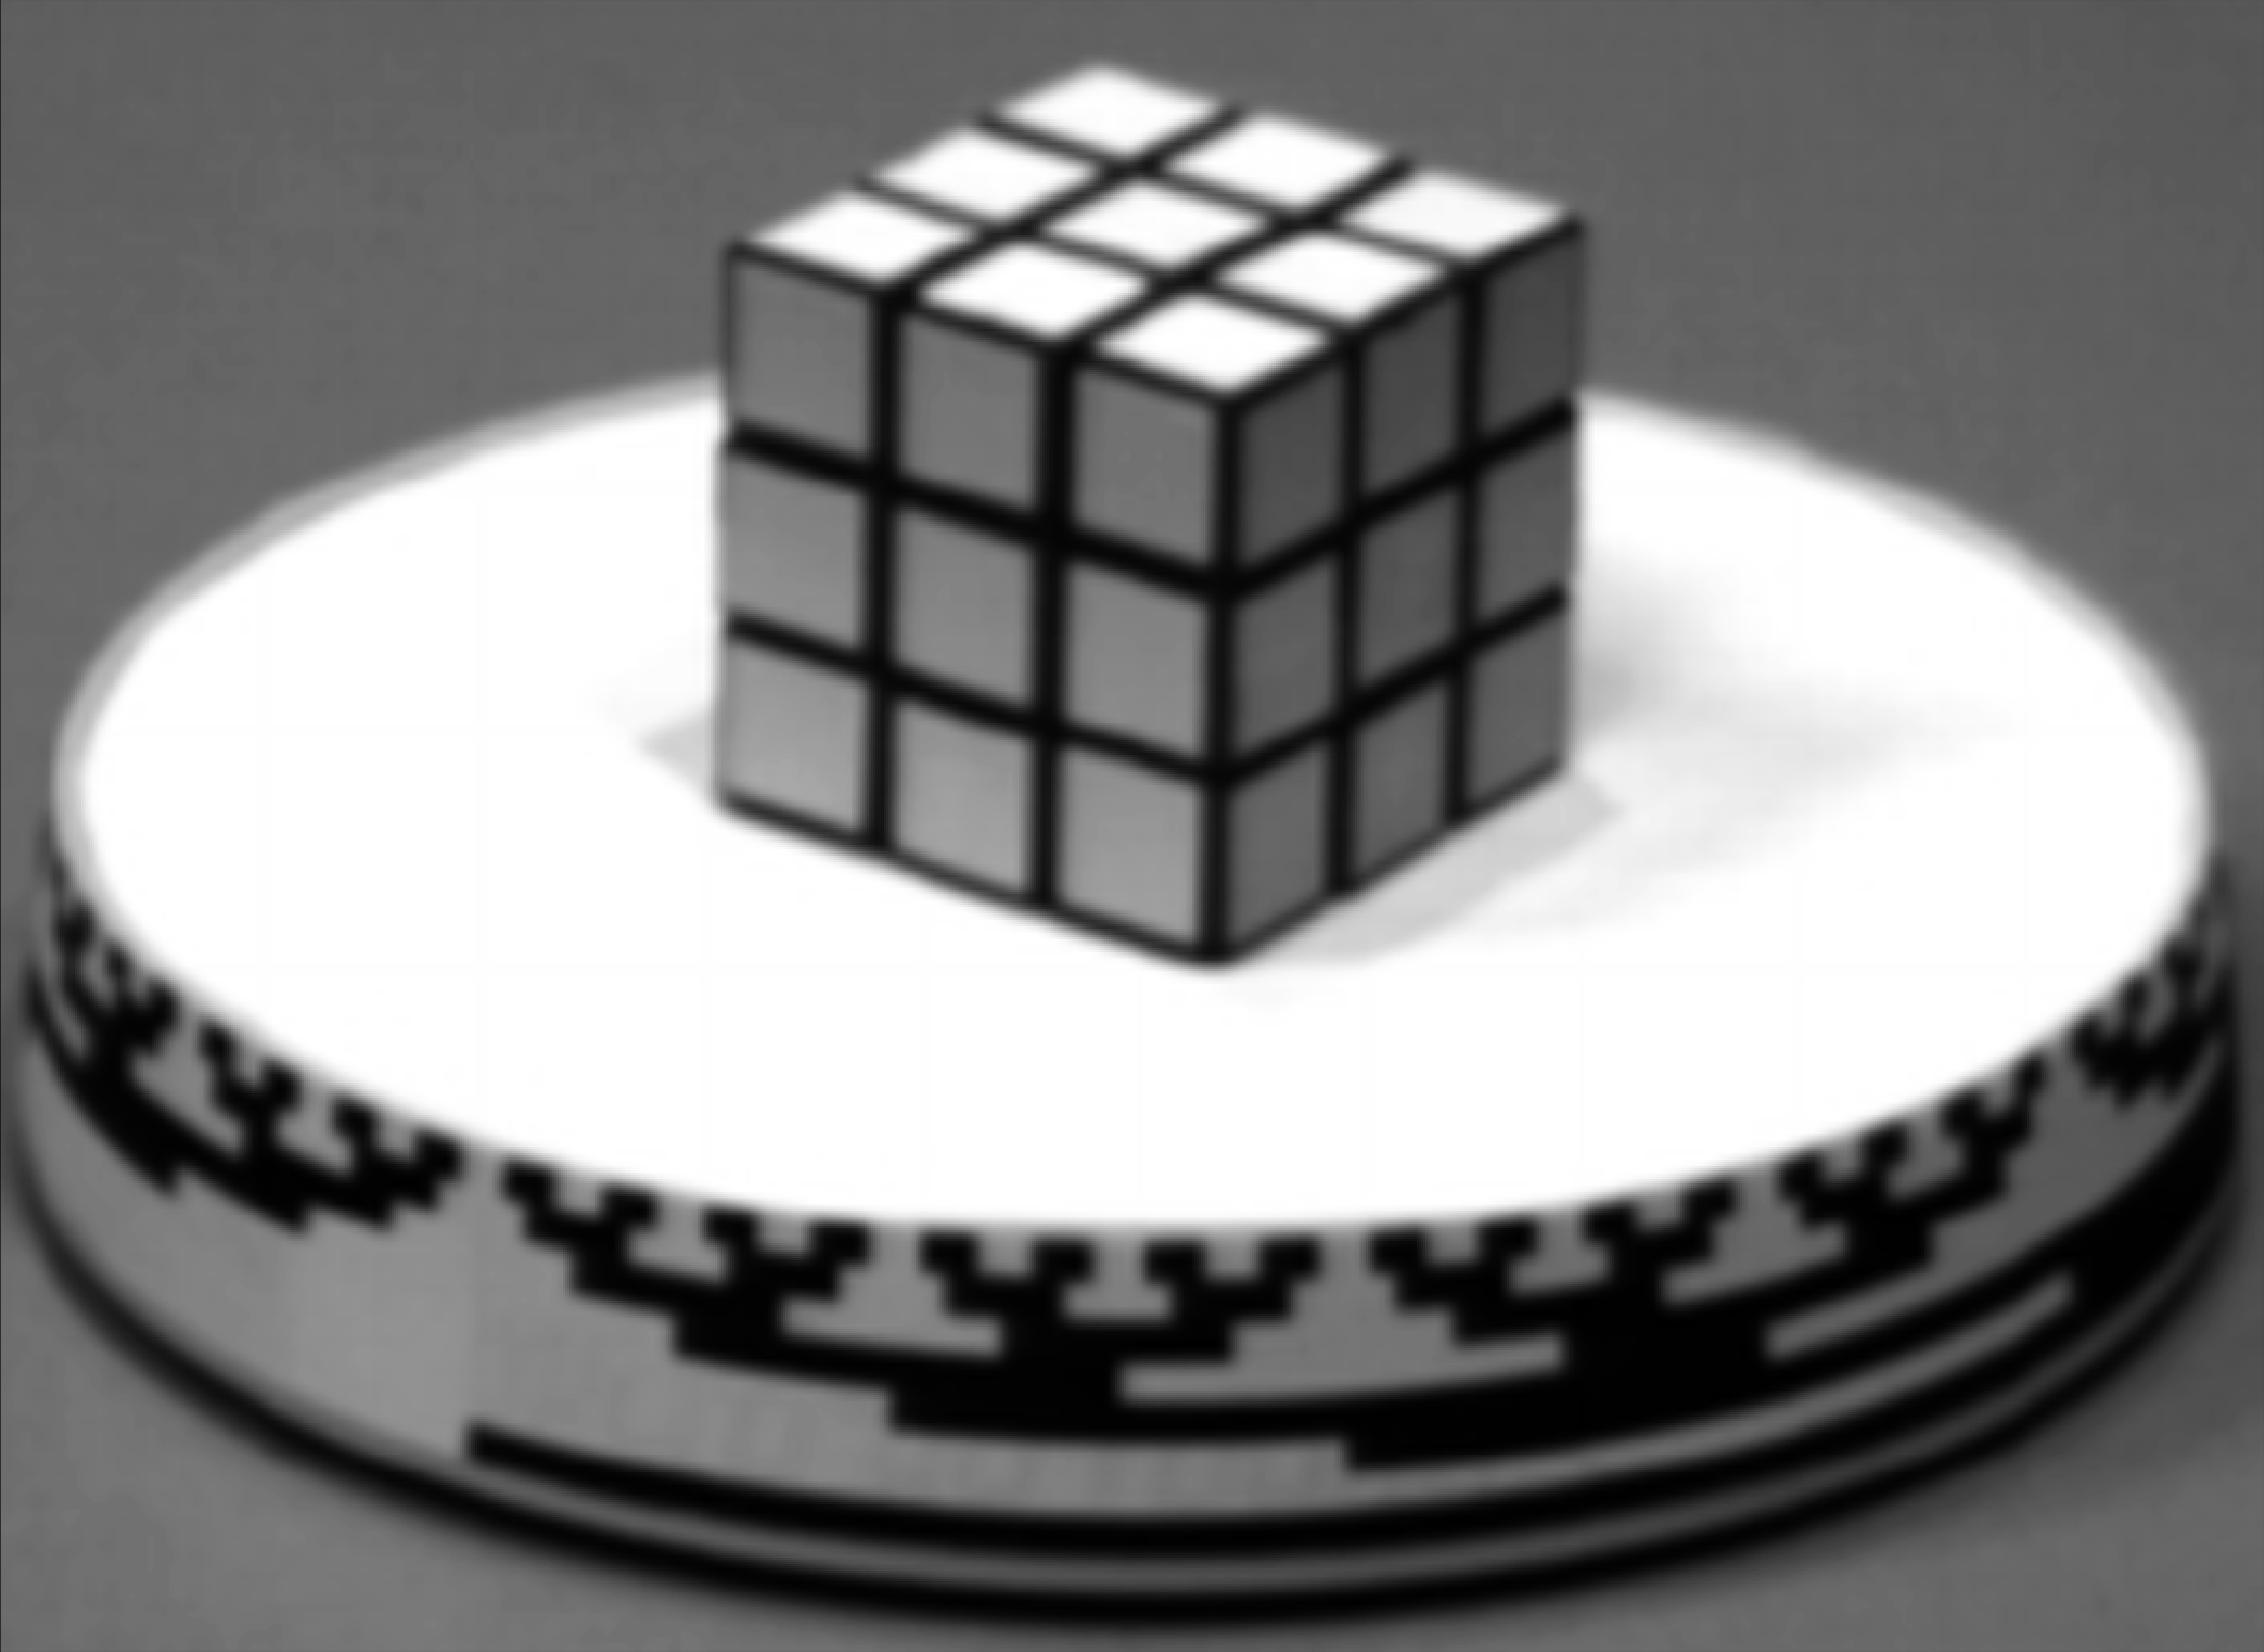
\includegraphics[]
			{figures/registration/optical_flow/moving_image.png}
		\end{adjustbox}
		\caption{Moving/displaced image.} \label{fig:movoptical}
	\end{subfigure}
	\vskip\baselineskip
	\begin{subfigure}{\linewidth}
		\centering
		\begin{adjustbox}{height=.7\textwidth}
			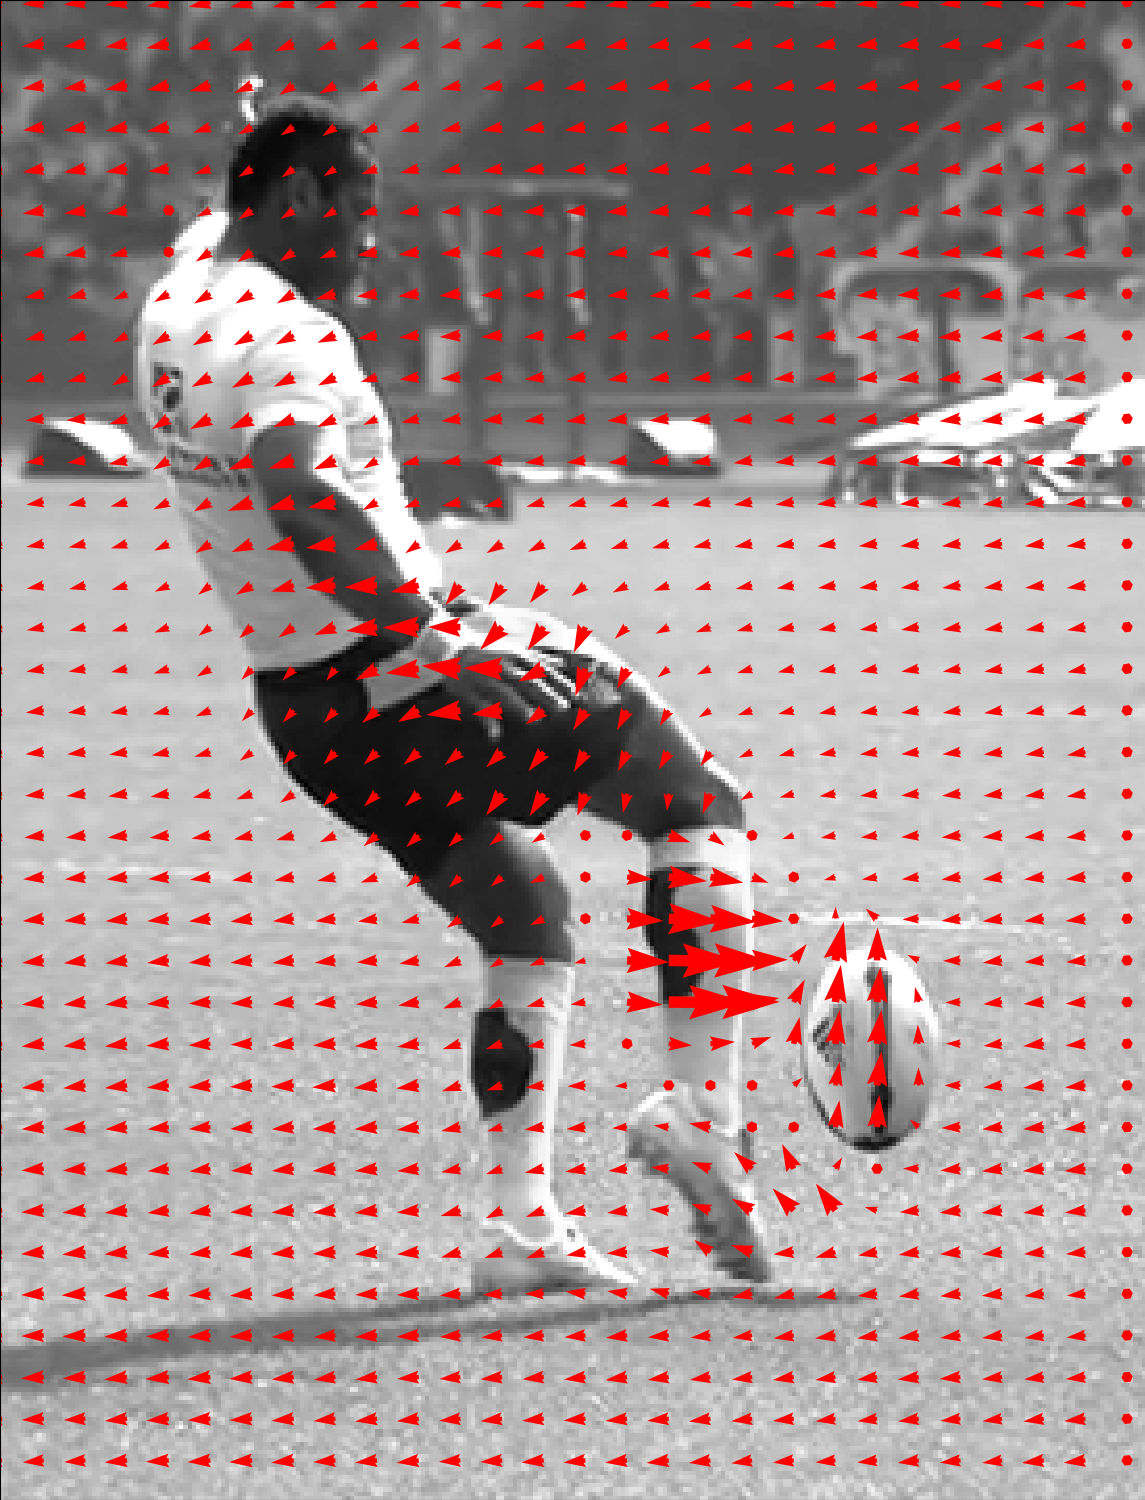
\includegraphics[]
			{figures/registration/optical_flow/flow.png}
		\end{adjustbox}
		\caption{Velocity field.} \label{fig:fieldoptical}
	\end{subfigure}
	\caption{Optical flow.}\label{fig:opticalflow}
\end{figure}

The most general and most interesting framing of the problem of local transformation is \textit{optical flow}.
%
Optical flow is the apparent motion of objects, surfaces, and edges in a scene caused by the relative motion between an observer and a scene.
%
It is most often represented as a velocity field over the individual point sources in the scene (see figure~\ref{fig:opticalflow}).
%
This velocity field can be used to define a mapping between pixels in the displaced image and the reference image (in a sense propagating the pixels backwards in time).

One approach to computing optical flow is based on treating pixel intensity as a \textit{conserved quantity}.
%
Let \(X(x,y,t)\) be pixel intensity over a sequence of images (i.e., the images per se).
%

\noindent Then define
\begin{equation*}
	Q(t) \coloneqq \iint_R X(x,y,t) \dif R
\end{equation*}
to be the total pixel intensity over some image region \(R\), and assume \(Q\) is differentiable in \(t\) (we deal with discretization in the forthcoming).
%
\(Q\) obeys an integral \textit{continuity equation}:
\begin{equation}
	\od{}{t} Q(t) + \oint_{\partial R} \mathbf{j} \cdot \mathbf{n}\, \dif l = \Sigma
	\label{eqn:intcontinuity}
\end{equation}
where \(\partial R\) is the closed boundary of \(R\), \(\dif l\) the differential line element of \(\partial R\), \(\mathbf{n}\) is unit length and normal to \(\partial R\), \(\mathbf{j}\) is the intensity flux (i.e., rate of flow of the intensity) through \(\partial R\), and \(\Sigma\) is the sum of all intensity sources and intensity sinks in \(R\).
%
Equation~\eqref{eqn:intcontinuity} expresses the fact that the change in total pixel intensity in the region \(R\) over time is equal to net intensity creation minus net flux through the boundary of the region.
%
By the Stokes' theorem\anote{stokes} and interchanging the order of integration and differentiation
%\begin{align}
%	\od{}{t} Q(t) + \oint_{\partial R} \mathbf{j} \cdot \mathbf{n}\, \dif l &=  \\
%	\od{}{t} \iint_R X(x,y,t) \dif R + \iint_R \nabla \cdot \mathbf{j}\, \dif R &= \\
%	 \iint_R \pd{X}{t} \dif R + \iint_R \nabla \cdot \mathbf{j}\, \dif R &= \\
%	\iint_R \pd{X}{t} + \nabla \cdot \mathbf{j}\,  \dif R &= \Sigma
%\end{align}
\begin{align*}
	\od{}{t} Q(t) + \oint_{\partial R} \mathbf{j} \cdot \mathbf{n}\, \dif l & = \od{}{t} \iint_R X(x,y,t) \dif R + \iint_R \nabla \cdot \mathbf{j}\, \dif R \\
	& = \iint_R \pd{X}{t} \dif R + \iint_R \nabla \cdot \mathbf{j}\, \dif R         \\
	& = \iint_R \left[ \pd{X}{t} + \nabla \cdot \mathbf{j} \right]  \dif R = \Sigma
\end{align*}
Then the differential form continuity equation corresponding to eqn.~\eqref{eqn:intcontinuity} is
\begin{equation}
	\pd{X}{t} + \nabla \cdot \mathbf{j} = \sigma
	\label{eqn:diffcontinuity}
\end{equation}
where now \(\sigma\) is net intensity creation per unit area.
%
This is a generalized advection equation\anote{advection}.
%
If pixel intensity is a conserved quantity (i.e., no net creation) eqn.~\eqref{eqn:diffcontinuity} becomes
\begin{equation}
	\pd{X}{t} + \nabla \cdot \mathbf{j} = 0
	\label{eqn:conservintent}
\end{equation}
By definition \(\mathbf{j} = X\mathbf{u}\) where \(\mathbf{u} \coloneqq (u_1(x,y), u_2(x,y))\) is the velocity field (over all the points in the image).
%
If we further assume that the intensity flow is incompressible (i.e., intensity density remains constant as it is advected by the point sources) then \(\nabla \cdot \mathbf{u} = 0\) and eqn~\eqref{eqn:conservintent} becomes
\begin{equation}
	\pd{X}{t} + \mathbf{u} \cdot \nabla X = 0
	\label{eqn:intensityconstr}
\end{equation}

Equation~\eqref{eqn:intensityconstr} is called the \textit{optical flow constraint equation}\cite{perez2013tv}.
%
Note that the constraint equation is a single linear equation in two unknowns (the components of \(\mathbf{u}\)) and is therefore under-determined.
%
\begin{figure*}
    \tikzset{
        aperture/.pic={
                \pgfmathsetmacro\cs{sqrt(1.5*cos(#1-45)^2/2)};
                \path [draw=black, rotate=#1, pattern=north east lines]
                    (-6/4,-6/2) rectangle (6/4,6/2);
                \path [fill=white, draw=black, even odd rule]
                    circle [radius=4/3] (-2,-2) rectangle (2,2);

                \draw[bluearrow, rotate=#1, line width=0.5mm] (0,0) -- node [above] {\small{\(\mathbf{u}\)}} (0,1.5);
                \draw[redarrow, line width=0.5mm] (0,0) -- node [above] {\small{\(\nabla X\)}} (-1.5,1.5);
                \draw[greenarrow, line width=0.5mm] (0,0) -- node [left] {\small{\(\nabla X \cdot \mathbf{u}\)}} (-\cs,\cs);
            }
    }
    \centering
    \begin{subfigure}[b]{0.3\textwidth}
        \centering
        \begin{adjustbox}{height=\textwidth}
            \begin{tikzpicture}
                \pic {aperture={45}};
            \end{tikzpicture}
        \end{adjustbox}
        \caption{Diagonal motion. \(\nabla X \cdot \mathbf{u}\) is maximum and therefore optical flow directly corresponds to motion.}
        \label{fig:diagbarber}
    \end{subfigure}
    \hfill
    \begin{subfigure}[b]{0.3\textwidth}
        \centering
        \begin{adjustbox}{height=\textwidth}
            \begin{tikzpicture}
                \pic {aperture={0}};
            \end{tikzpicture}
        \end{adjustbox}
        \caption{Vertical motion. \(\nabla X \cdot \mathbf{u}\) is less than maximum and therefore optical flow fails to capture all of the motion.}
        \label{fig:vertbarber}
    \end{subfigure}
    \hfill
    \begin{subfigure}[b]{0.3\textwidth}
        \centering
        \raisebox{22pt}{
            \begin{adjustbox}{width=\textwidth}
                \begin{tikzpicture}
                    \pic {aperture={90}};
                \end{tikzpicture}
            \end{adjustbox}
        }
        \caption{Horizontal motion. \(\nabla X \cdot \mathbf{u}\) is less than maximum and therefore optical flow fails to capture all of the motion.}
        \label{fig:horizbarber}
    \end{subfigure}
    \caption{Barber-poll illusion. Each of the three motion measure as vertical optical flow.}
    \label{fig:barberpoll}
\end{figure*}
%
This is called the \textit{aperture problem} or the Barber-poll illusion (see figure~\ref{fig:barberpoll}) because any motion perpendicular to image gradients \(\nabla X\) (i.e., edges) isn't captured by the constraint: to wit if 
\[\mathbf{u}' \cdot \nabla X= 0\] 
then 
\[
	\pd{X}{t} + \left(\mathbf{u} + \mathbf{u}' \right) \cdot \nabla X = \pd{X}{t} + \mathbf{u} \cdot \nabla X = 0
\]
%
Therefore additional constraints need to be imposed in order to uniquely determine \(\mathbf{u}\).
%
The first such additional constraint was the \textit{spatial coherence constraint} proposed by Lucas \etal\cite{lucas1981iterative}: assume a pixel's neighbors have the same velocity \(\mathbf{u}\).
%
For example using a \(5 \times 5\) window around a given pixel yields a \(5\times5 = 25\) equation over-determined system (solved using least-squares).

Regularizers can also be used to resolve the aperture problem. 
%
Defining \(\rho(\mathbf{u})\) as the left-hand side of eqn.~\eqref{eqn:intensityconstr}, Horn \etal\cite{horn1993determining} propose the functional
\begin{equation}
	E(\mathbf{u}) \coloneqq \int_R \left[ \abs{\rho(\mathbf{u})}^2 + \alpha \left( \abs{ \nabla u_1 }^2 + \abs{ \nabla u_2 }^2\right) \right] \dif R
	\label{eqn:linearhorn}
\end{equation}
where \(\abs{ \nabla u_1 }^2\) is the \(L_2\) norm of \(\nabla u_1 = (\pd{u_1}{x}, \pd{u_1}{y})\).
%
\(E(\mathbf{u})\) acts a smoothing regularizer, constraining the acceleration of the flow (recall that \(\mathbf{u}\) is the velocity of the flow).
%
Note that \(\nabla u_1\) is not the first component of \(\nabla \cdot \mathbf{u} = (\pd{u_1}{x}, \pd{u_2}{y})\) and therefore not identitically zero (despite the assumption that  \(\nabla \cdot \mathbf{u} = 0\)).

Although eqn.~\eqref{eqn:intensityconstr}, along with Horn smoother, is an effective resolution to the problem of computing optical flows in continuous time it is unsuitable for images sampled discretely in time.
%
In such cases eqn.~\eqref{eqn:intensityconstr} is replaced by \( X_k(\bx + \mathbf{u}) - X_1(\bx)\), where \(\bx = (x,y)\), and then \( X_k(\bx + \mathbf{u})\) is  linearized around an initial velocity \(\mathbf{u}_1\) to produce a discrete constraint equation:
\begin{multline}
	\nabla X_k (\bx + \mathbf{u}_1)\cdot (\mathbf{u} - \mathbf{u}_1)\, + \\ X_k(\bx + \mathbf{u}_1)  -  X_1(\bx) = 0
	\label{eqn:nonlinearconstr}
\end{multline}
Defining \(\rho'(\mathbf{u})\) as the left-hand side of eqn.~\eqref{eqn:nonlinearconstr}, the Horn smoother suitably adjusted is
\begin{equation}
	E'(\mathbf{u}) \coloneqq \int_R \left[ \abs{ u_1 }^2 + \abs{ u_2 }^2 + \lambda \abs{ \rho'(\mathbf{u}) }_1 \right] \dif R
	\label{eqn:nonlinearhorn}
\end{equation}
%
Perez \etal\cite{perez2013tv} further relax this to a convex loss:
\begin{multline}
	E_{\theta}(\mathbf{u}, \mathbf{v}) \coloneqq \\
	\int_R \left[ \abs{ u_1 }^2 + \abs{ u_2 }^2 + \frac{1}{2\theta}\abs{ \mathbf{u} - \mathbf{v} }^2 + \lambda \abs{ \rho'(\mathbf{v}) }_1 \right] \dif R
	\label{eqn:relaxhorn}
\end{multline}
in order that they can alternate fixing one of \(\mathbf{u}, \mathbf{v}\) and minimizing with respect to the other.
%
Note that fixing \(\theta\) in eqn.~\eqref{eqn:relaxhorn} to be small pushes \(E_{\theta}(\mathbf{u}, \mathbf{v})\) to be small when \(\mathbf{u}\approx \mathbf{v}\) and therefore effectively minimizes eqn.~\eqref{eqn:nonlinearhorn}.
\paragraph{Splines}
\begin{figure}
    \centering
    \begin{subfigure}[b]{0.49\textwidth}
        \centering
        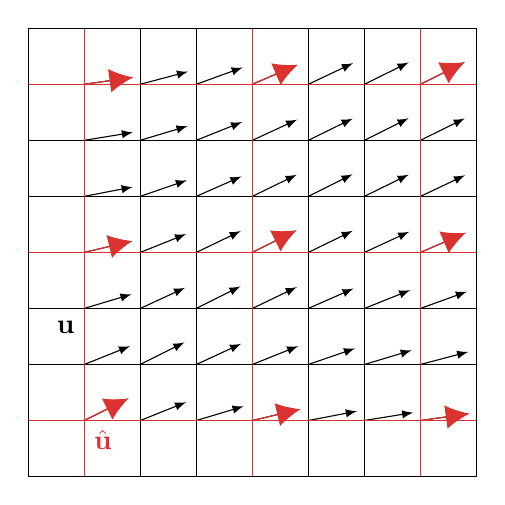
\begin{tikzpicture}
            \def\length{sqrt((x^2+y^2)^2  + (x*y)^2 )}
            \begin{axis}[
                    enlargelimits = false ,
                    view={0}{90},
                    xmin=0, xmax=1, ymin=0, ymax=1,
                    ytick distance=1/8,
                    xtick distance=1/8,
                    axis equal image,
                    grid=both,
                    major grid style={black},
                    axis equal image,
                    ticks=none
                ]
                \addplot3[
                    domain=1/8:7/8,
                    black,
                    quiver={
                            u={(x^2+y^2)/\length},
                            v={x*y/\length},
                            scale arrows=0.11
                        },
                    -latex,
                    samples=7
                ] {0};
            \end{axis}
            \begin{axis}[
                    enlargelimits = false ,
                    view={0}{90},
                    xmin=0, xmax=1, ymin=0, ymax=1,
                    xtick={1/8,1/2,7/8},
                    ytick={1/8,1/2,7/8},
                    axis equal image,
                    grid=both,
                    major grid style={red},
                    axis equal image,
                    ticks=none
                ]
                \addplot3[
                domain=1/8:7/8,
                red,
                quiver={
                        u={(x^2+y^2)/\length},
                        v={x*y/\length},
                        scale arrows=0.11
                    },
                -{Latex[length=3mm,width=3mm]},
                samples=3
                ] {0};
                \node  at  (axis cs:1/8,1/8)  [anchor=north west, red] {\(\hat{\mathbf{u}}\)};
                \node  at  (axis cs:1/8,3/9)  [left, black] {\(\mathbf{u}\)};
            \end{axis}
        \end{tikzpicture}
        \caption{Spline interpolation for the velocity field.}\label{fig:bsplinegrid}
    \end{subfigure}
    \vskip\baselineskip
    \begin{subfigure}[b]{0.49\textwidth}
        \centering
        \def\centerx{2}
        \def\centery{-1}
        \begin{tikzpicture}
            \begin{axis}
                \addplot3[surf,domain=-2:6,domain y=-5:3]
                {exp(-( (x-\centerx)^2 + (y-\centery)^2)/3 )};
            \end{axis}
        \end{tikzpicture}
        \caption{Biquadratic spline basis function}\label{fig:biquadspline}
    \end{subfigure}
    \caption{Spline interpolation for velocity fields.}
\end{figure}
One issue with optical flow methods is that they are very compute intensive; iteratively minimizing either eqn.~\eqref{eqn:nonlinearhorn} or eqn.~\eqref{eqn:relaxhorn} requires evaluations at every pixel.
%
Splines offer an efficient alternative to estimating \(\mathbf{u}\) at every pixel.
%
A \textit{spline} is a piece-wise defined polynomial function. For example a simple \textit{order} \(d+1\) spline \(s\) could be defined
\[
		s(x) = \sum_{i=0}^d \mathbbm{1}_{[k_j, k_{j+1})}P_{ij} \cdot (x - k_j)^i
\]
where the \(n+1\) increasing \textit{knots} \(k_0 < \cdots < k_n\) bracket \(n\) intervals over which the component polynomials are defined, and the \((d+1)\) polynomial coefficients \(P_{ij}\) define the spline (see figure~\ref{fig:cubicspline}) for \(x \in [k_j, k_{j+1})\) (\(\mathbbm{1}\) enforces this\anote{indicator}).
%
Splines need not be differentiable (nor even continuous) at the knots but can be specified with such continuity constraints (at the knots).
%
The number of degrees of freedom of a spline over \(n+1\) knots and of order \(d+1\) (i.e., the dimension of the vector space\anote{vectorspace} of such splines) is the number of polynomial coefficients minus the number of continuity conditions
%
For example if the spline is constrained to be maximally continuous (i.e., continuous and differentiable \(d-1\) times\anote{splinecontconstr}) then the spline has \(d+1\) polynomial coefficients for every one of the \(n\) knot intervals and \(d\) continuity constraints at every one of the \(n-1\) interior knots (continuity constraints cannot be specified at the boundary knots), which implies 
\[
	n(d+1) - (n-1)d = n+d
\]
degrees of freedom. The spline construction naturally extends to dimensions greater than 1.

Szeliski \etal~\cite{szeliski1997spline} represent the velocity field \(\mathbf{u}\) as a two-dimensional spline controlled by a smaller number of displacement estimates \(\hat{\mathbf{u}}\) at control points, which lie on a coarser grid (see figure~\ref{fig:bsplinegrid}):
%
\begin{equation}
	\begin{bmatrix}
		u_1(x,y) \\ u_2(x,y)
	\end{bmatrix} = \sum_j \begin{bmatrix}
		\hat{u}_{1j}(x,y) \\ \hat{u}_{2j}(x,y)
	\end{bmatrix} B_j(x, y)
\end{equation}
where \(B_j\) are \textit{basis functions}. 
%
In particular they experiment with basis functions such as the biquadaritc B-spline:
\[
	B_j(x,y) = B_{j,2}(x) B_{j,2}(y)
\]
where \(B_{j,2}\) is the quadratic B-spline (defined in the forthcoming and displayed in figure~\ref{fig:biquadspline}).

As an alternative one can completely forgo optical flow and simply perform Free-Form Deformation\cite{xie2004} using \textit{Basis splines} (B-splines).
%
A B-spline is a spline defined as a linear combination of a particular set of basis functions (themselves called B-splines): the B-spline basis element \(B_{i, d+1}\) of order \(d+1\) (degree \(d\)) over knots \(k_i < \cdots < k_{i+d+1}\) is defined recursively according to the Cox-de Boor recursion formula\cite{de1971subroutine}:
\begin{align}
	B_{j,1} (x) &= \mathbbm{1}_{[k_j, k_{j+1})} \\
	B_{j,d+1} (x) &= \frac{x-k_j}{k_{j+d} - k_j} B_{j,d} (x) \\
	&\quad+ \frac{k_{j+d+1} - x}{k_{j+d+1} - k_{i+1}} B_{j+1,d} \nonumber (x)
\end{align}
where \(\frac{x-k_j}{k_{j+d} - k_j}\) increases smoothly from zero to one as \(x\) goes from \(k_j\) to \(k_{j+d}\) and \(\frac{k_{j+d+1} - x}{k_{j+d+1} - k_{i+1}}\) decreases smoothly from one to zero as \(x\) goes from \(k_{i+1}\) to \(k_{j+d+1}\).
%
Xie \etal\cite{xie2004} fit hierarchical B-splines 
\begin{equation}
	\mathbf{s}(x,y) = \sum_{i=0}^m\sum_{j=0}^n \mathbf{P}_{ij} B_{i,3}(x) B_{j,3}(y)
\end{equation}
on a regular knot grid (see figure~\ref{fig:bicubicspline}).
%
This makes the splines purely functions of the coefficients \(\mathbf{P}_{ij}\) rather than the knots and coefficients both (as is typically the case).
%
Note the coefficients here control the contribution of each component B-spline.
%
Their solution is hierarchical in that after the initial fit they check goodness and refine by inserting knots and recomputing.
%
They use the hierarchically fit spline to interpolate at points outside the set of control points matched during the control point matching step of the registration process.
%
\begin{figure}
    \centering
    % \begin{subfigure}[b]{0.49\textwidth}
    %     \centering
    %     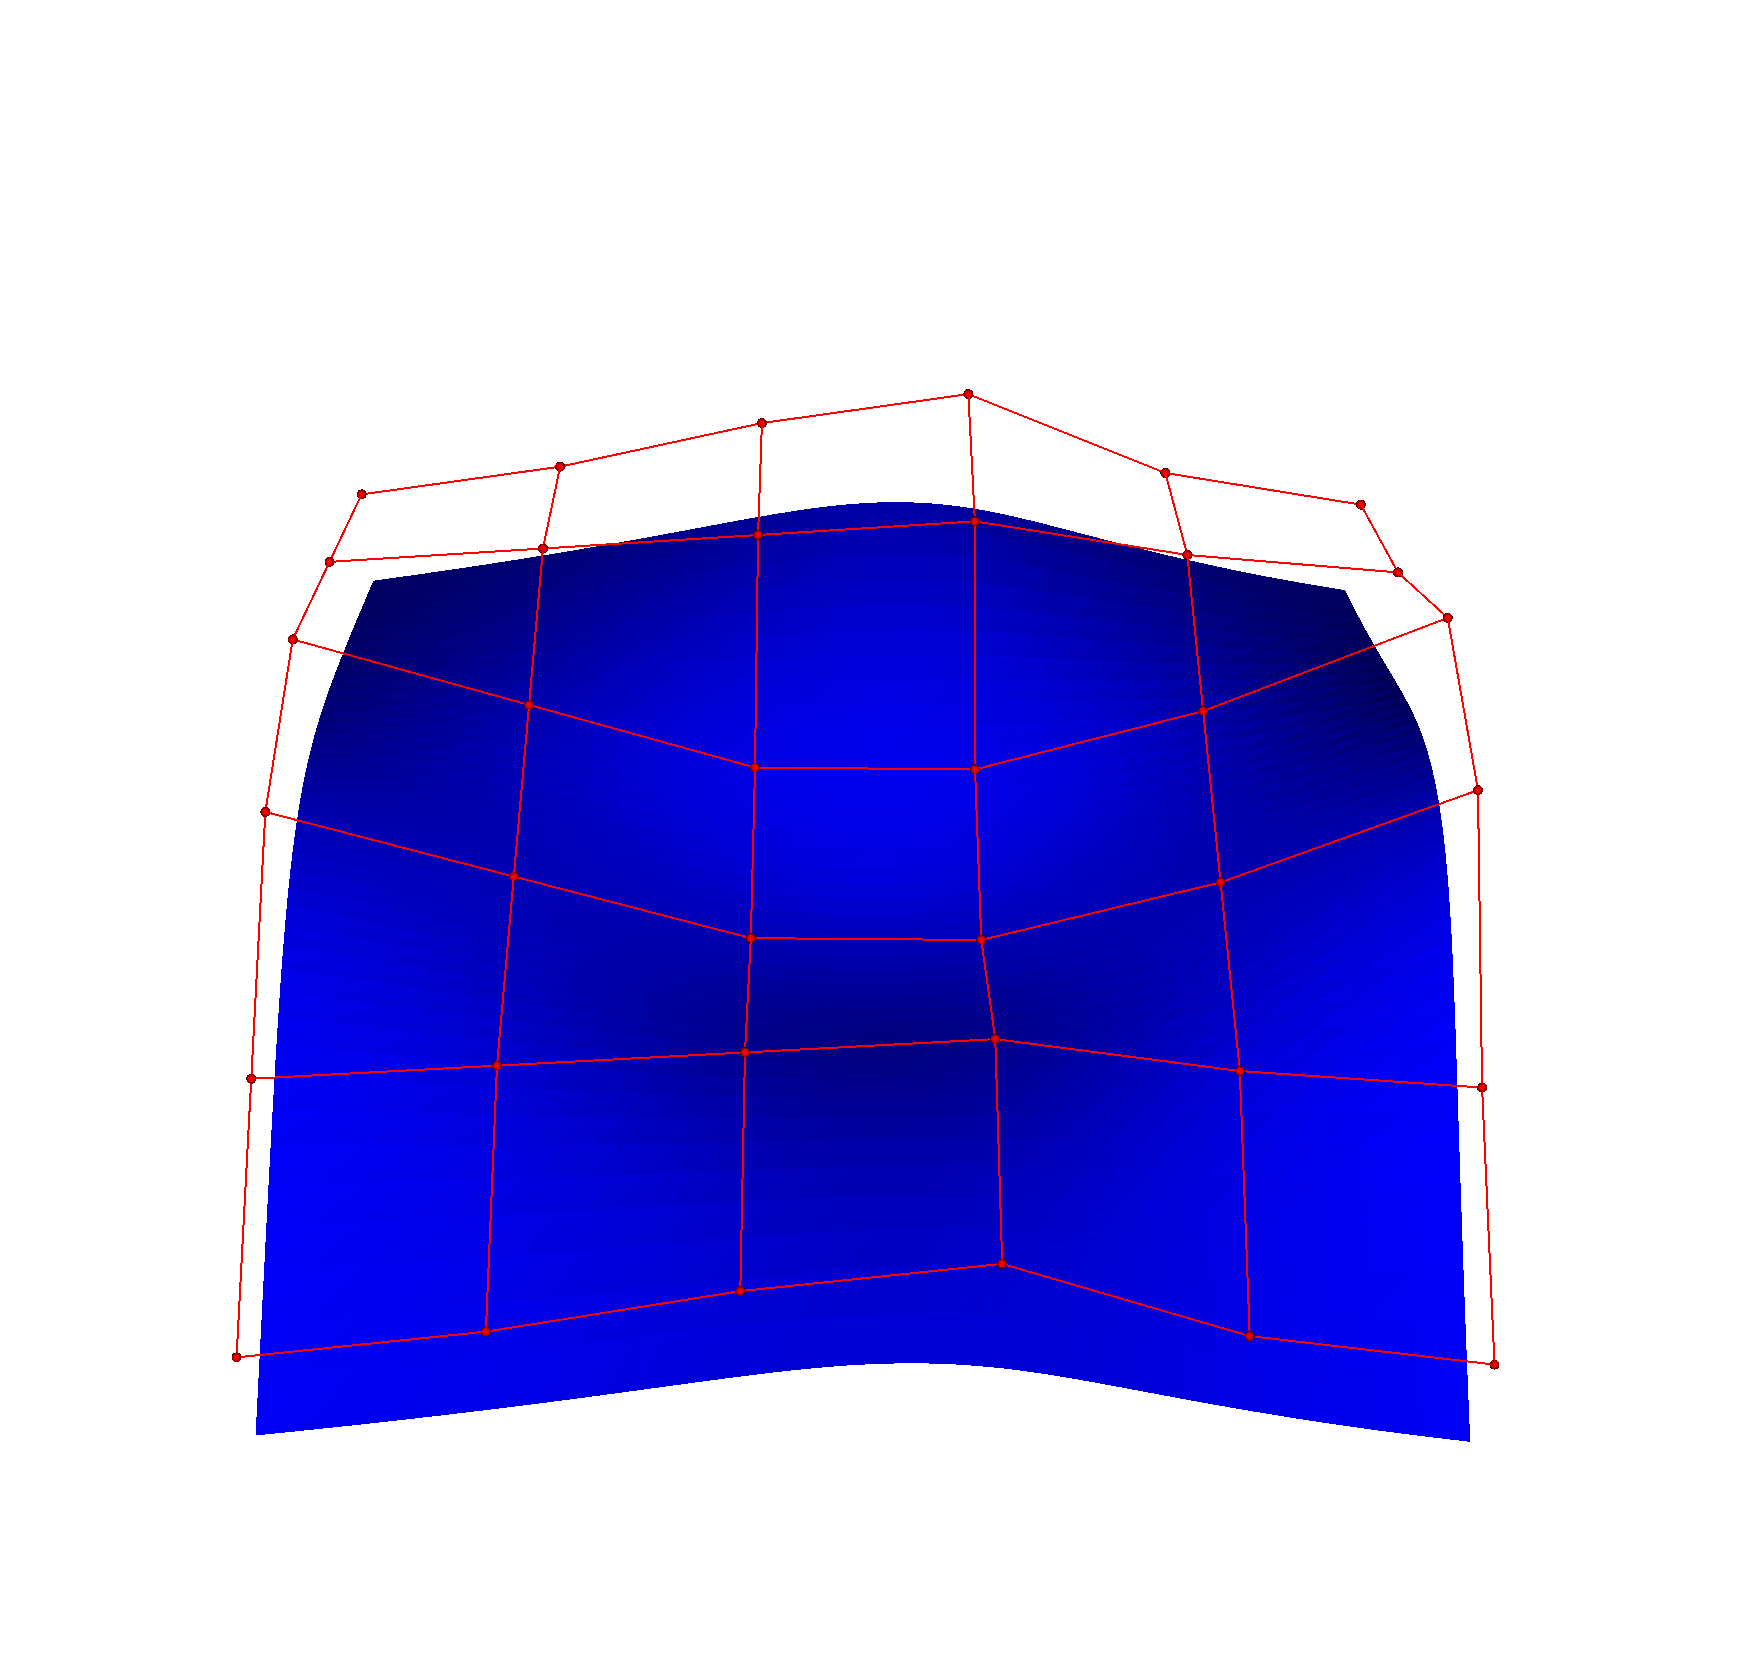
\includegraphics[height=\textwidth, trim=90 90 90 90, clip]{figures/registration/splines/spline2.png}
    % \end{subfigure}
    \begin{subfigure}[b]{0.49\textwidth}
        \centering
        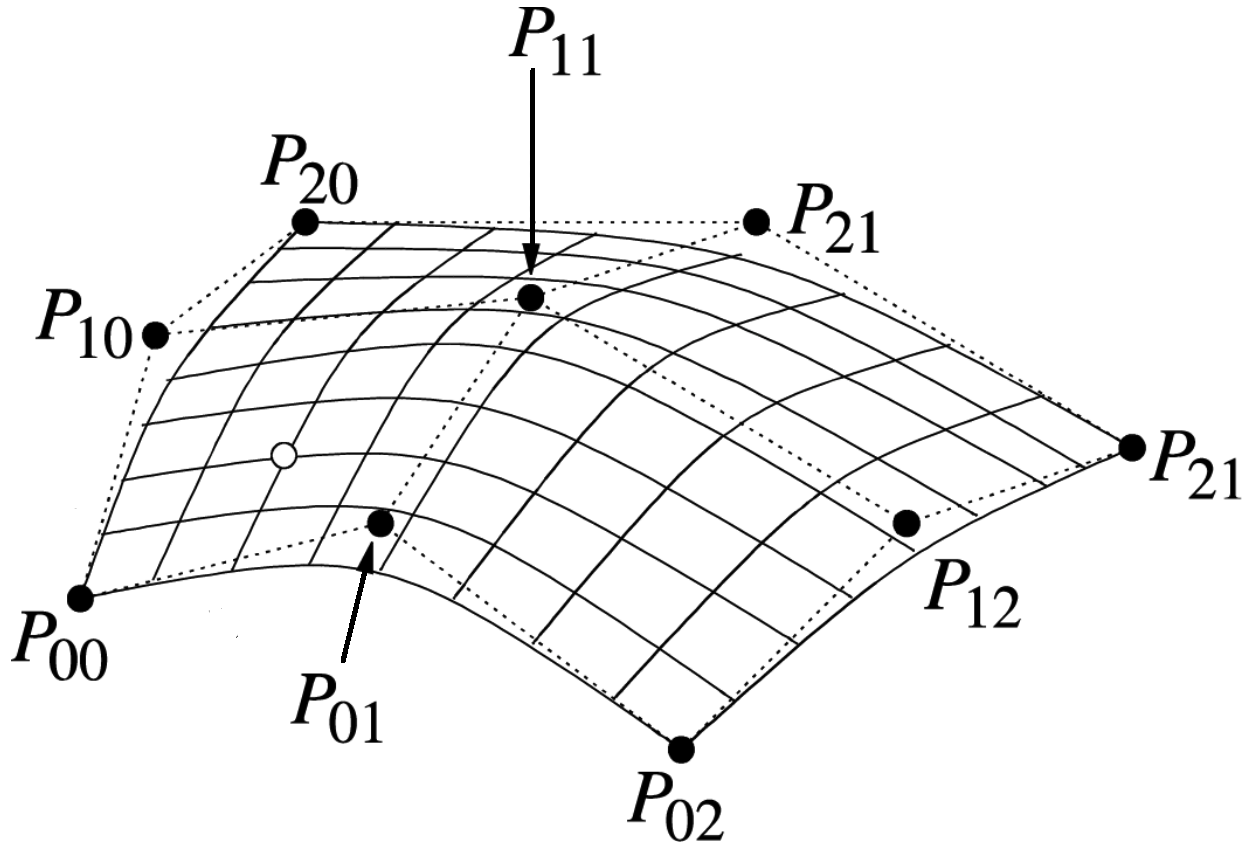
\includegraphics[height=.6\textwidth]{figures/registration/splines/spline5.png}
        \caption{Bicubic spline}
        \label{fig:bicubicspline}
    \end{subfigure}
    \vskip\baselineskip
    \begin{subfigure}[b]{0.49\textwidth}
        \centering
        \begin{adjustbox}{width=.6\textwidth}
            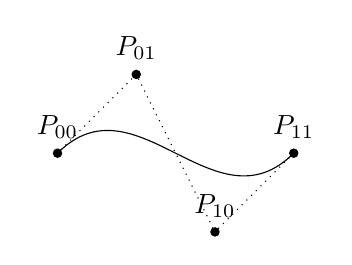
\begin{tikzpicture}
                \tikzset{
                    ctrlpoint/.style={%
                            draw=black,
                            fill,
                            circle,
                            inner sep=0,
                            minimum width=3pt,
                        }
                }
                \newcommand\Bezier[4]{% \bezier (lowercase 'b') was already defined elsewhere
                    \node (p1) [ctrlpoint,label=90:$P_{00}$] at (#1) {};
                    \node (p2) [ctrlpoint,label=90:$P_{01}$] at (#2) {};
                    \node (p3) [ctrlpoint,label=90:$P_{10}$] at (#3) {};
                    \node (p4) [ctrlpoint,label=90:$P_{11}$] at (#4) {};
                    \draw [black, dotted] (p1) -- (p2) -- (p3) -- (p4);
                    \draw [black] (#1) .. controls (#2) and (#3) .. (#4);
                }
                \Bezier{0,0}{1,1}{2,-1}{3,0}
            \end{tikzpicture}
        \end{adjustbox}
        \caption{Cubic spline}
        \label{fig:cubicspline}
    \end{subfigure}

    % \begin{subfigure}[b]{0.49\textwidth}
    %     \centering
    %     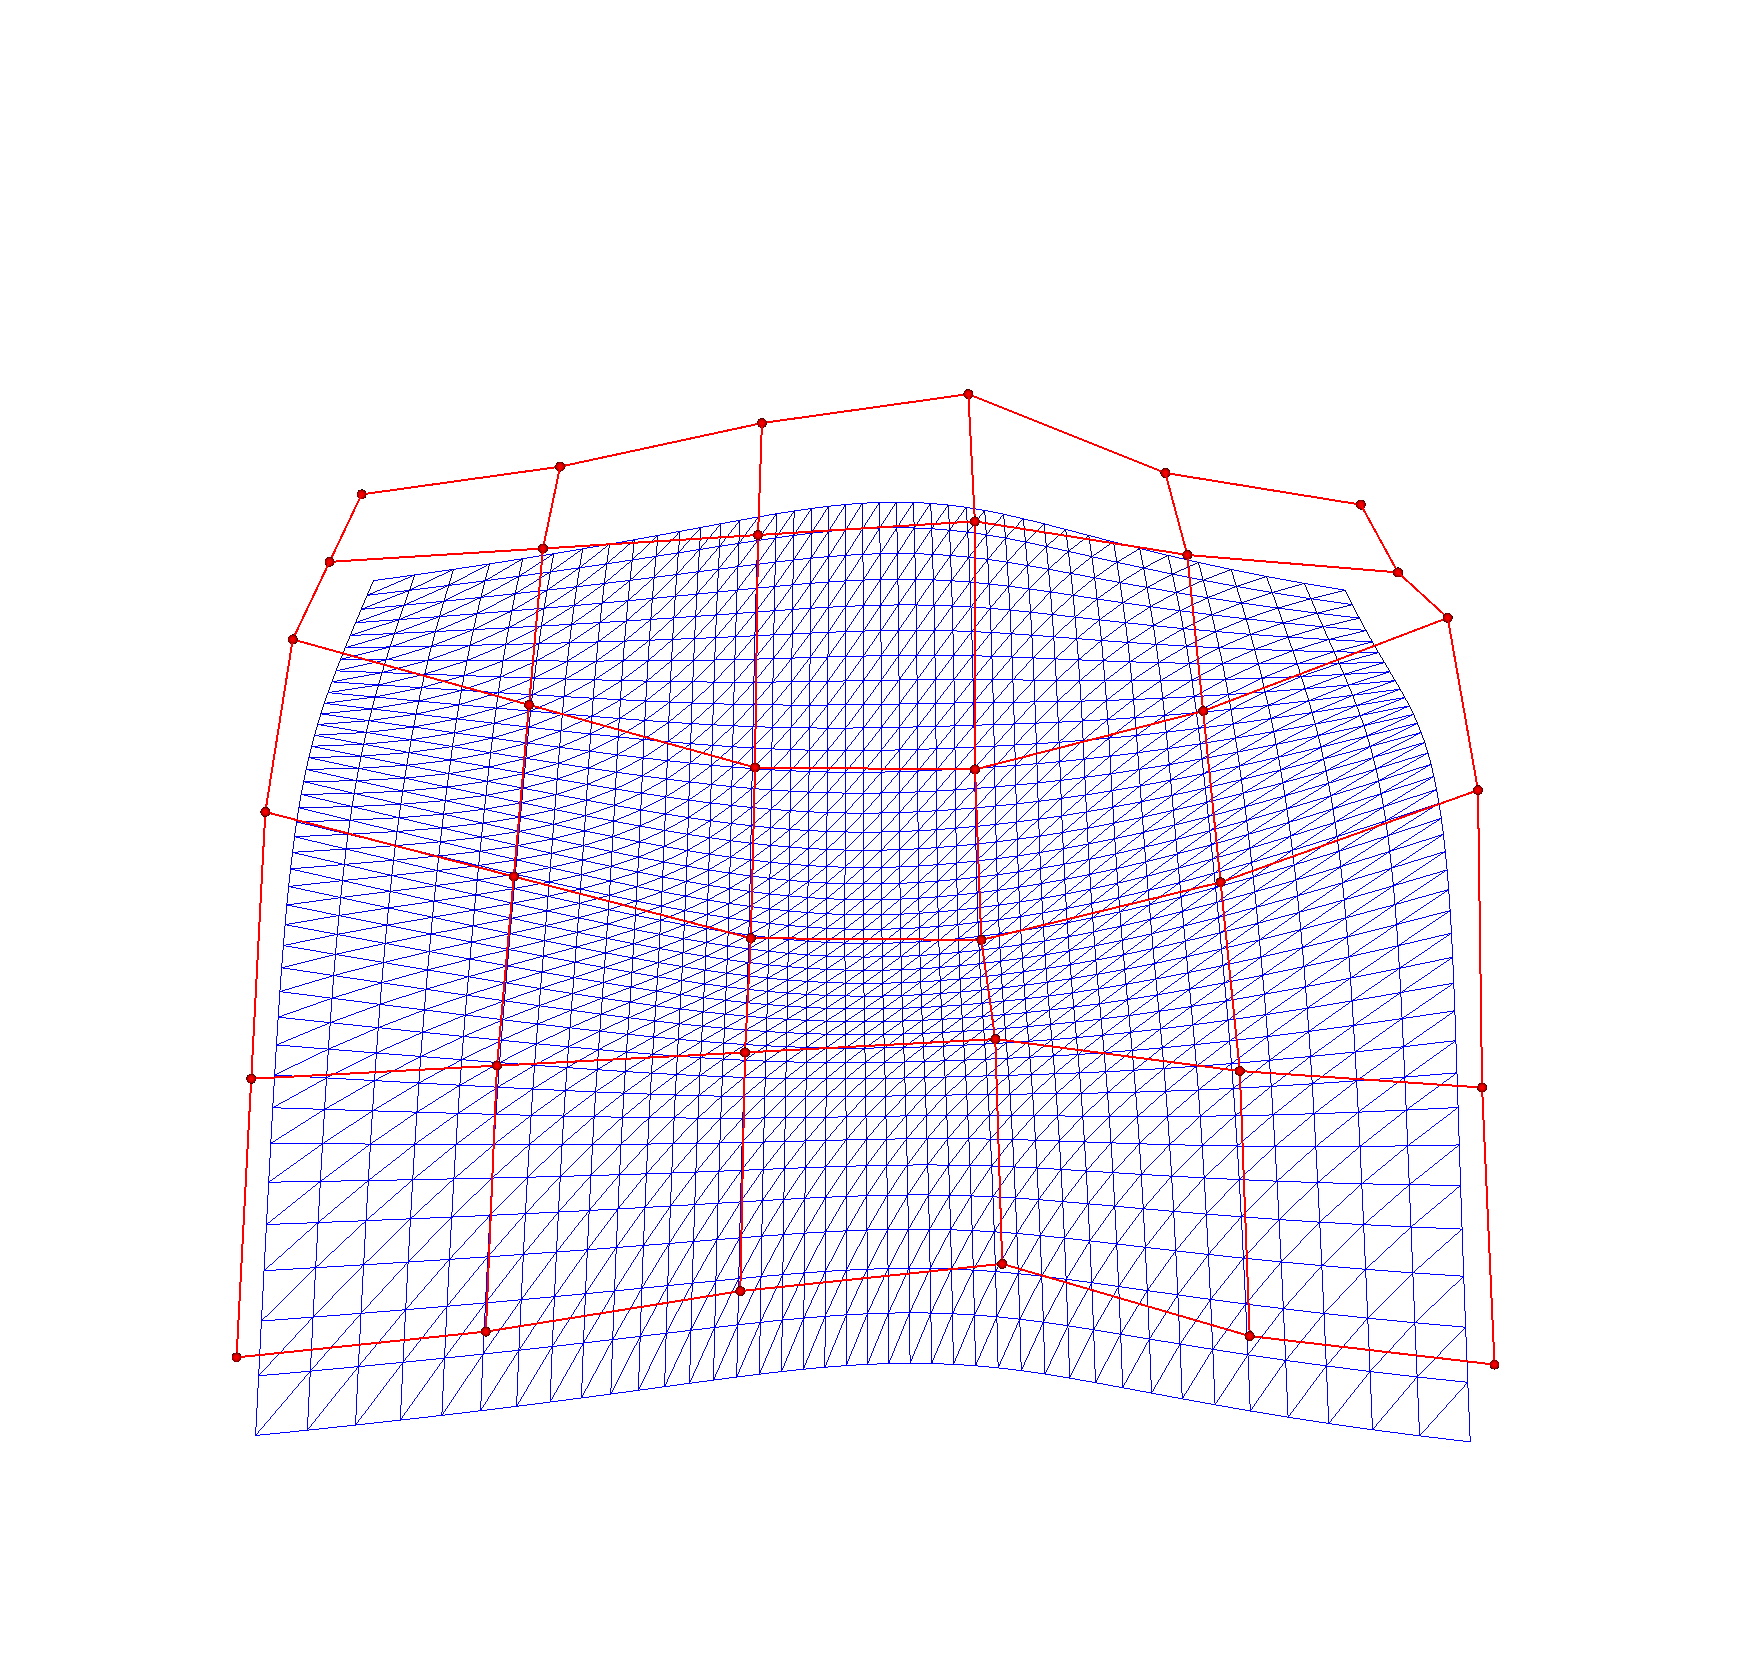
\includegraphics[height=\textwidth, trim=90 90 90 90, clip]{figures/registration/splines/spline3.png}
    % \end{subfigure}
    \caption{Splines with control points emphasized.}
    \label{fig:spline}
\end{figure}

\newpage
\subsection{Interpolation}\label{subsec:interpolation}

Suppose that $H_k$ is linear spatial\anote{lsi} and time invariant.
%
Suppose further that $A_k$ is affine.
%
Then $H \coloneqq H_k$ commutes with $A_k$\cite{meladcommute} and eqn.~\eqref{eqn:commuteimagingmodel} becomes
\begin{equation}
	\label{eqn:commuteimagingmodel}
	\begin{split}
		\Xk &= (D \circ A_k \circ H) (Y) + \varepsilon \\
		&= (D \circ A_k) (H(Y)) + \varepsilon \\
		&= (D \circ A_k) (V) + \varepsilon
	\end{split}
\end{equation}
%
where $V \coloneqq H(Y)$.
%
This naturally suggests interpolation in order to recover $V$ (since $\Xk$, in this framing, is simply shifted samples of $V$).
%
Note in this context we use interpolation very broadly, i.e. to connote filling in missing values using neighboring (in some sense --- not necessarily geometrically) values.
%
\begin{figure}
	\centering
	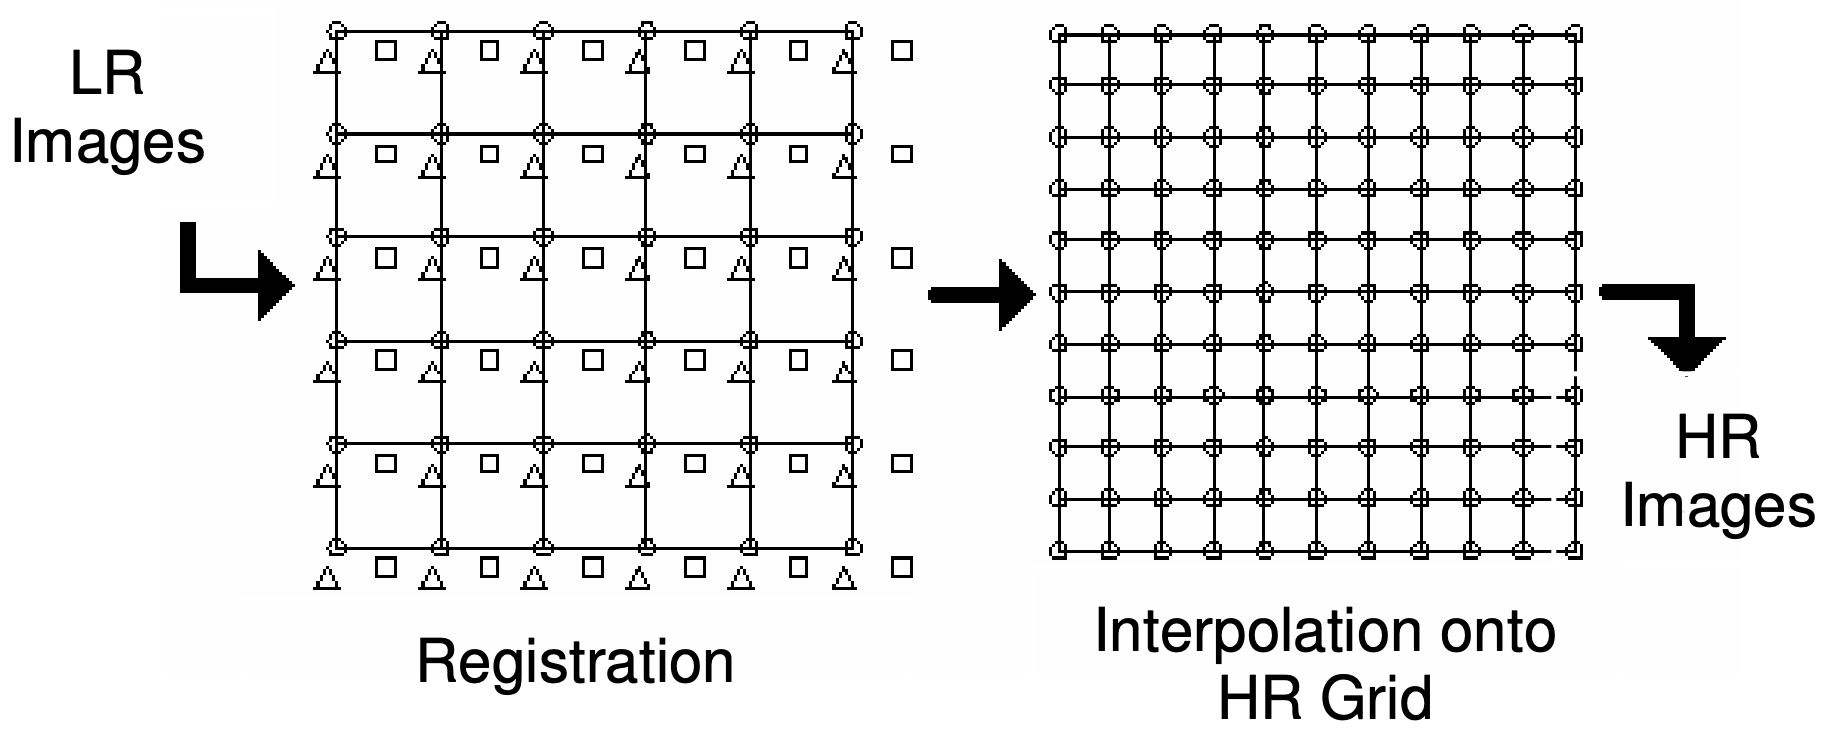
\includegraphics[width=\linewidth,keepaspectratio]{figures/classical/hrgrid.png}
	\caption{LR image registration on an HR grid\cite{Lin}}
	\label{fig:hrgrid}
\end{figure}
This class of techniques proceed by first registering images on a high resolution grid (see figure~\ref{fig:hrgrid}) then interpolating at the "missing" pixels in the HR grid to recover $V$, and finally denoising and deconvolution (of $H$) to recover $Y$.
%
Since in general consecutive $\Xk$ have non-uniform shifts (relative to $X_1$) the interpolation is non-uniform and improvisations on this theme use various weighting schemes for adjacent LR pixels\anote{lrpixel}.

For example Alam \text{et al.}\cite{Alam2000} uses weighted nearest neighbors: for every pixel to be interpolated the three nearest pixels are weighted inversely by their distance (according to HR grid distance) and then their weighted sum is assigned to that pixel.
%
This non-uniform interpolation is then followed by application of a Wiener filter whose design is informed by the OTF of the particular imaging system they study (which they do not estimate i.e. they assume they can model accurately).
%
\subsubsection{Delaunay Triangulation}

\begin{figure}
	\centering
	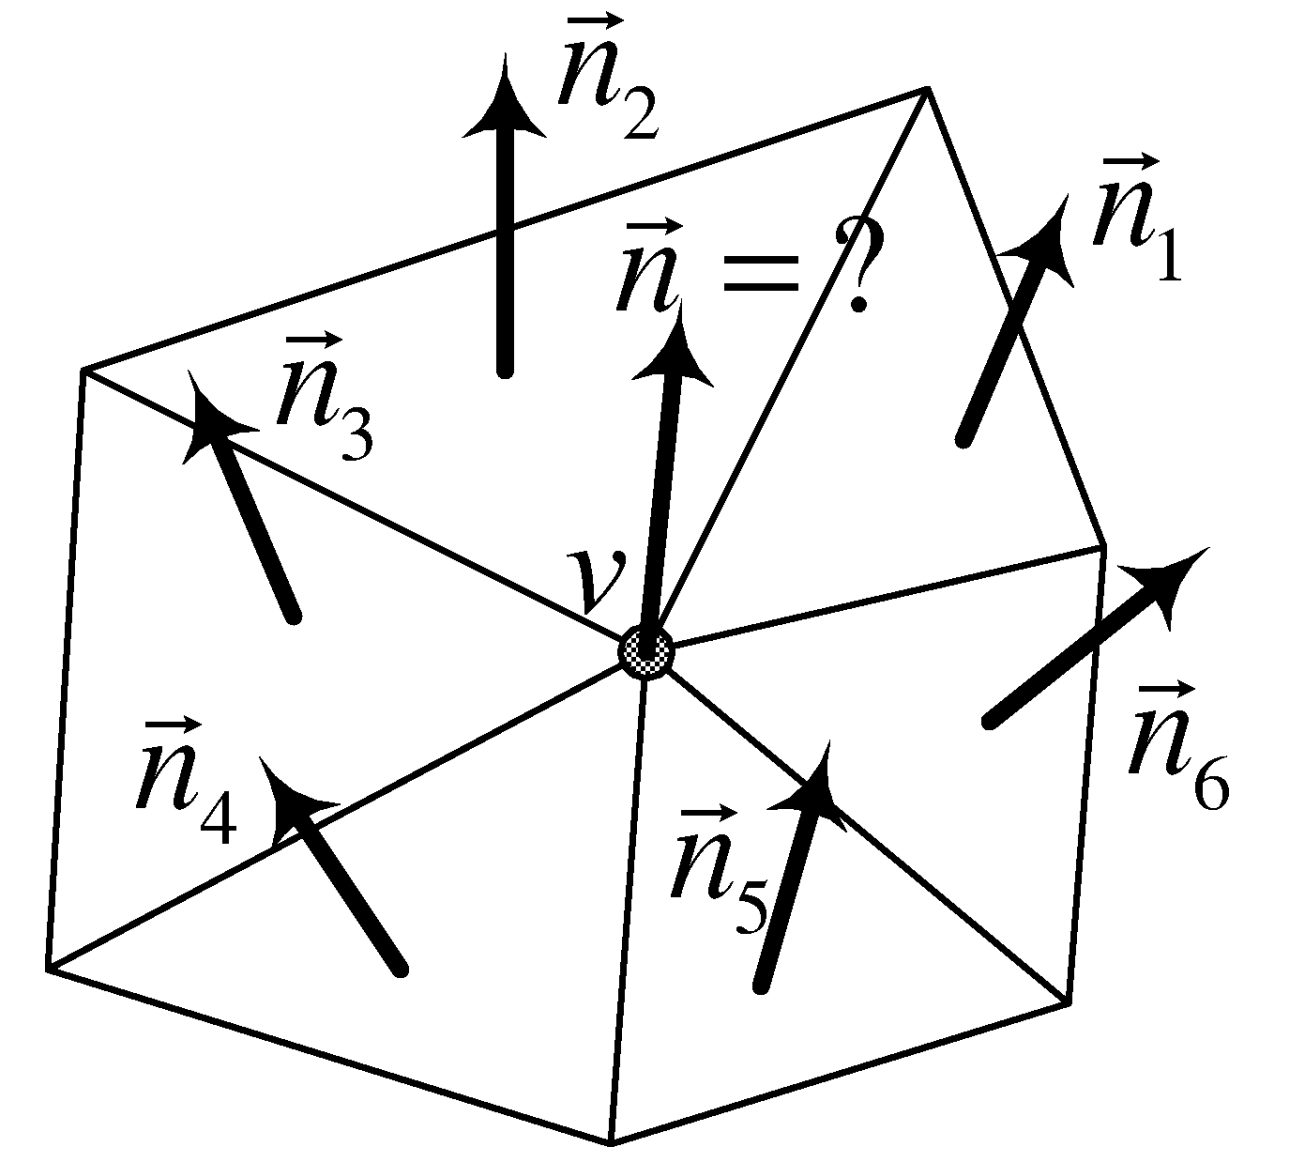
\includegraphics[width=.7\linewidth]{figures/classical/delauney.png}
	\caption{Delaunay triangulation for fitting splines at LR pixels\cite{Lertrattanapanich}. $v$ is an LR pixel. Note that $v$ is at $z$ equal to the pixel value}
	\label{fig:delauney}
\end{figure}
Lertrattanapanich \text{et al.}\cite{Lertrattanapanich} base their algorithm on interpolants which require knowledge of gradients (e.g. splines) and mediate the non-uniform sampling by using a weighted average (by area) of those gradients in adjacent Delaunay cells; to be precise they produce a Delaunay triangulation of all LR pixels and compute the gradients (see figure~\ref{fig:delauney}) according to
\begin{align*}
	\vec{n} = \sum_{i=1}^m \frac{B_j \vec{n_j}}{B}   & \text{ where } B=\sum_{i=1}^m B_i                              \\
	\frac{\partial z}{\partial x} = -\frac{n_x}{n_z} & \text{ and }  \frac{\partial z}{\partial y} = -\frac{n_y}{n_z}
\end{align*}
where $B_i$ is the area of the $i$th Delaunay cell.
%
Unfortunately this intricate solution is not robust to noise in real images.
\subsubsection{Wiener Filter}
A more sophisticated method for non-uniform interpolation uses parametric models for the auto-correlation between LR pixels and the cross-correlation between LR pixels and interpolated pixels to estimate wiener filter weights\cite{wiener}.
%
These weights are then used to average nearby pixel values.
%
The algorithm operates on a sliding \textit{estimation window} whose dimensions $D_x, D_y$ are chosen such that the effective sampling rate exceeds the Nyquist rate for a given $\rho_c$.
\begin{figure}
	\centering
	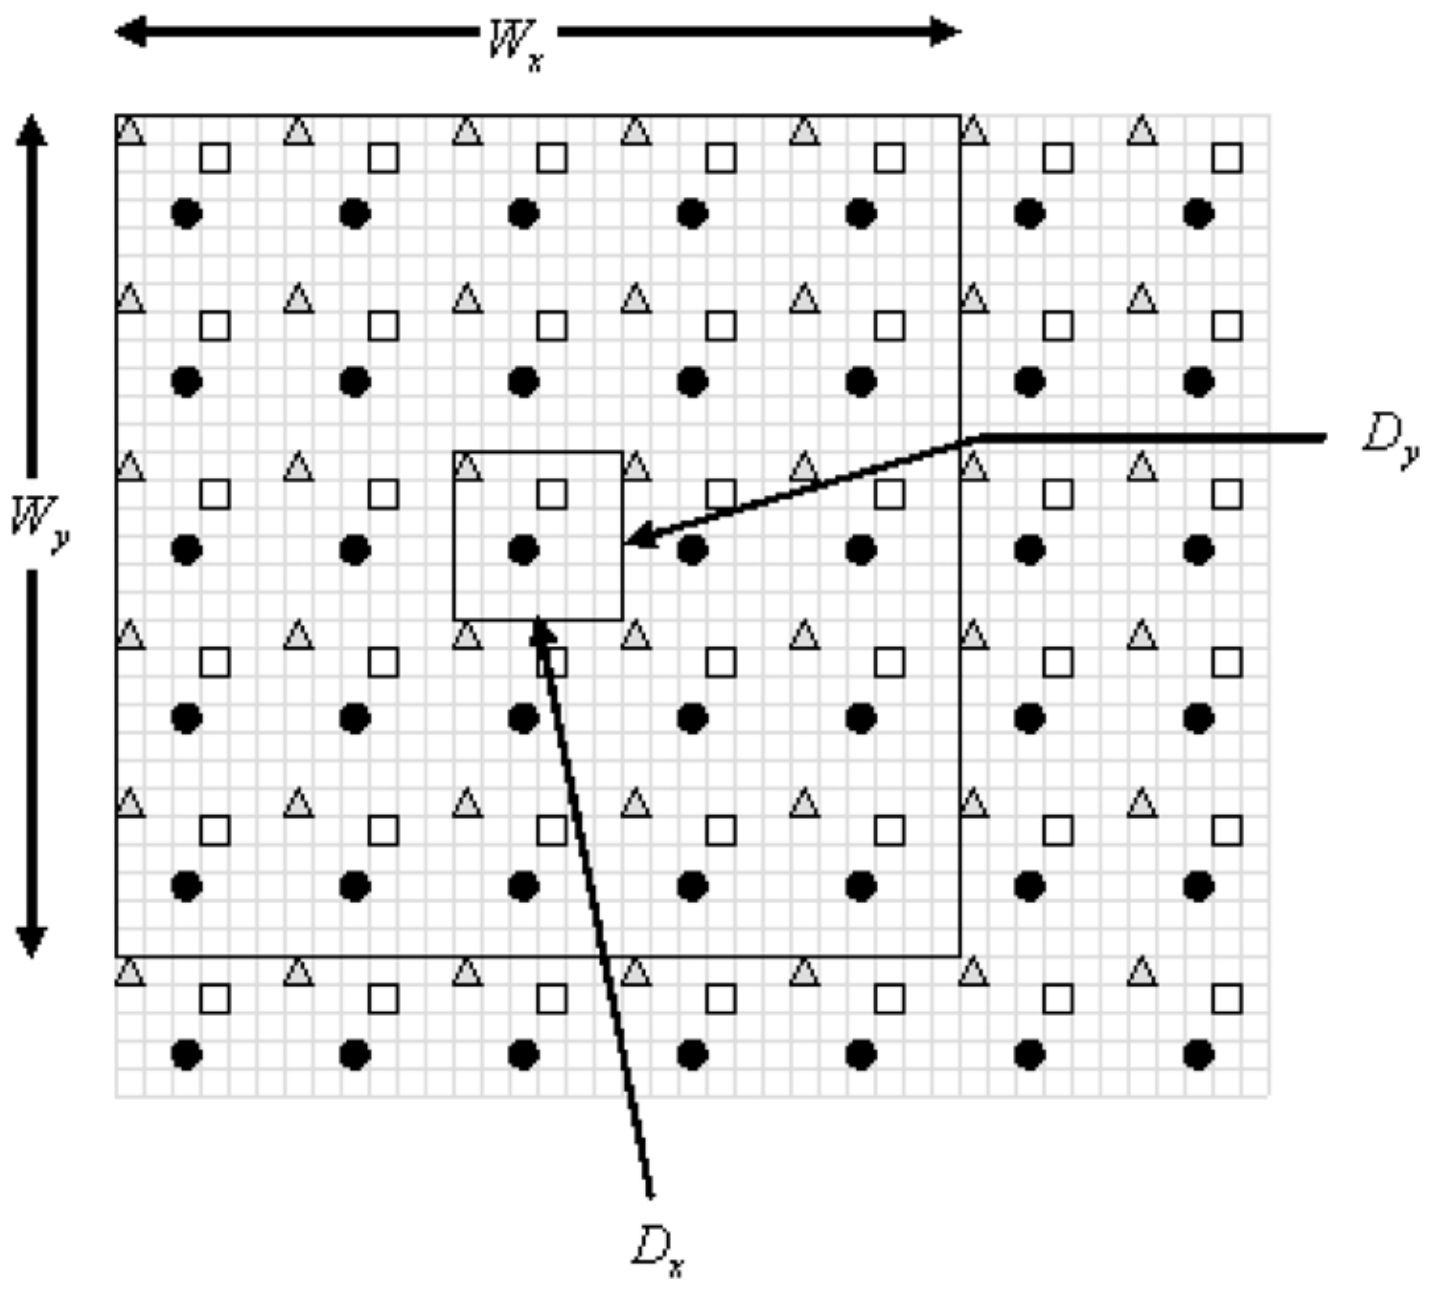
\includegraphics[width=.7\linewidth]{figures/classical/wiener.png}
	\caption{Wiener filter super resolution estimation window of dimension $D_x \times D_y$ and observation window of dimension $W_x \times W_y$\cite{wiener}}
	\label{fig:wiener}
\end{figure}
The pixel values for the estimation window are a function of the wiener filter weights of nearby LR pixels within an \textit{observation window} whose dimensions $W_x, W_y$ are an integer multiple of $D_x, D_y$ (see figure~\ref{fig:wiener}).
%
The weights $\bm{w}$ are defined as the solution to the minimum mean squared error (MMSE) filter problem, i.e. the finite impulse response (FIR) wiener filter:
\begin{equation}
	\bm{w} = R^{-1}\bm{p}
\end{equation}
where $R$ is the auto-correlation of the LR pixels in the observation window and $\bm{p}$ is the cross-correlation between the pixels to be estimated and the LR pixels.
%
Then $R$ and $\bm{p}$ are both constructed by sampling a parametric model that weights pixels in the observation window according to distance:
%
$R$ is constructed by sampling from
\begin{equation}
	C_1(r) \coloneqq \sigma_{d}^2 \rho^{r} \ast G(r)
\end{equation}
and $\bm{p}$ is constructed by sampling from
\begin{equation}
	C_2(r) \coloneqq \sigma_d^2 \rho^{r} \ast G(r) \ast G(-r)
\end{equation}
In the case of $R$, $r$ is distance on the HR grid, $\sigma_d$ is related to the empirical variance of all LR pixels in a given observation window and $G(r)$ is a smoothing kernel (e.g. Gaussian).
%
Thus by evaluating $C_1$ for all $r = r(n_1, n_2)$ distances between LR pixels $n_1$, $n_2$ we can construct $R$.
%
Similarly for $\bm{p}$, $r = r(m, n)$ is the distance between pixel-to-be-estimated $m$ and LR pixel $n$.
%
Note that $R$ is an $N \times N$ matrix where $N = K W_x W_y/D_x D_y$, i.e. how many LR pixels there are in the observation window, and $\bm{p}$ is an $N \times 1$ column vector uniquely computed for each pixel in the estimation window.
%
The scheme is effective but suffers from issues with the spatial isotropy of the auto-correlation and cross-correlation models.
\subsubsection{Steering Kernels}
One of the most sophisticated of these non-uniform interpolation schemes employs the kernel regression framework and \textit{steering kernels} (see~\ref{fig:steering}).
%
In this context we start with all $\Xk$ registered to a common HR grid and consider pixel values $Y(\bxi)$ at pixel coordinates $\bxi \coloneqq (x_{i1},x_{i2})$ as the measured data pairs $(\bxi, Y(\bxi)$.
%
Recall that kernel regression frames the estimation problem as
\begin{equation}
	Y(\bxi) = Z(\bxi) + \varepsilon
\end{equation}
where $Z$ is the to-be-estimated \textit{regression function} that "predicts" $Y$ as a function of $\bx$.
Then the Nadaraya–Watson estimator (NWE)\cite{Nadaraya} $\hat{Z}$ for $Z$ is
\begin{equation}
	\hat{Z}(\bx) = \frac{\sum_{i=1}^{P}K(\delx)Y(\bxi)}{\sum_{i=1}^{P}K(\delx)}
	\label{eqn:kernelregression}
\end{equation}
where $P$ indexes over all pixels in the HR grid and $K$ is a \textit{kernel function} whose purpose is to decay the contribution of $\bxi$ if it's in some sense far from $\bx$.
%
Note that $\hat{Z}(\bx)$ can also be seen as a weighted filtering of $Y$.
%
\begin{figure}
	\centering
	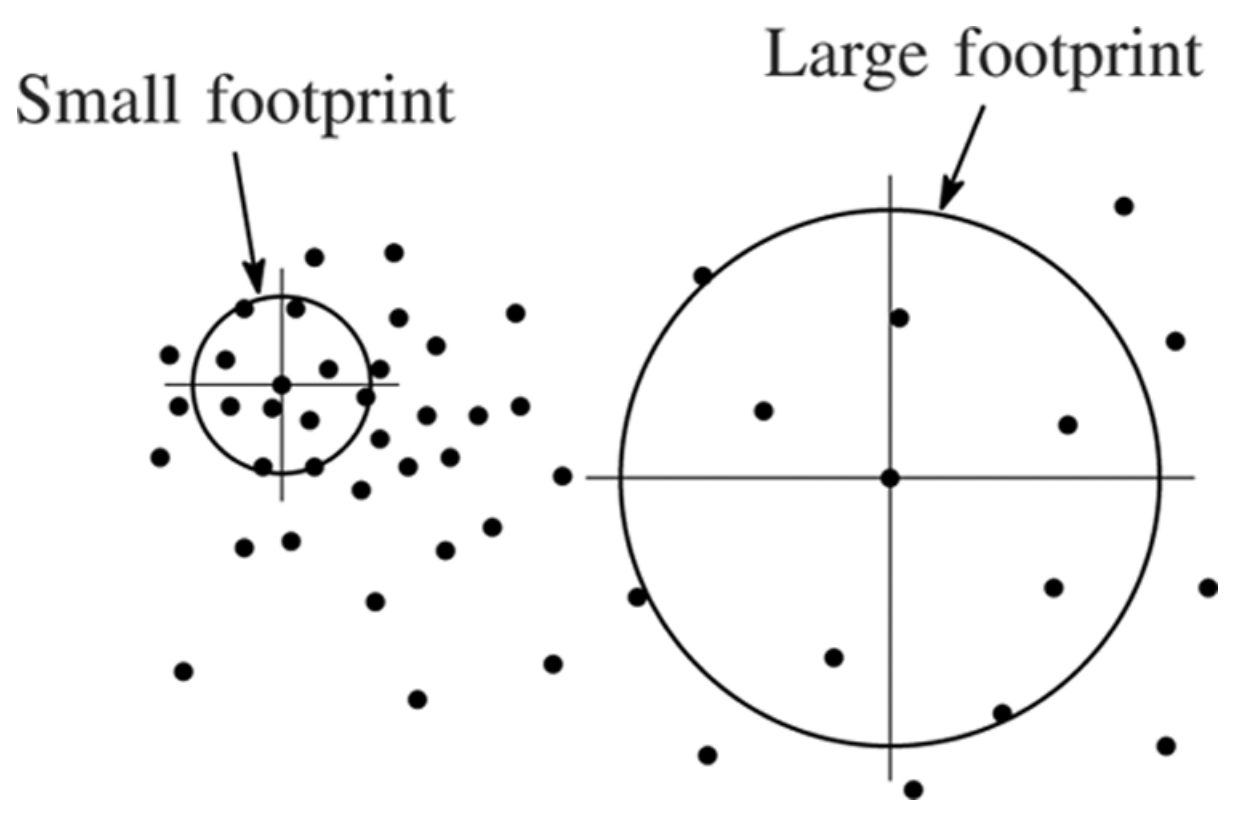
\includegraphics[width=.8\linewidth]{figures/classical/footprint.png}
	\caption{Kernel footprint as a function of sample density\cite{Takeda2007}}
	\label{fig:footprint}
\end{figure}
\begin{figure}
	\centering
	\includegraphics[width=\linewidth,keepaspectratio]{figures/classical/steering.png}
	\caption{Adapting kernel shape as a function of local directed structure\cite{Takeda2007}}
	\label{fig:steering}
\end{figure}
In conventional kernel regression $K$ might be any non-negative, symmetric, unimodal\cite{wand1994kernel} function with augmented with an additional $h$ parameter that controls the "bandwidth" or "footprint" of the kernel, i.e.
\begin{equation}
	K_h(\delx) \coloneqq \frac{1}{h}K\left( h^{-1}(\delx) \right)
\end{equation}
This bandwidth parameter $h$ can be generalized to a \textit{smoothing kernel} $H$ in order to make $K = K_H$ adaptive to the local structure of the pixels, e.g. to have larger footprints in sparsely sampled regions and have smaller footprints in densely sampled regions (see figure~\ref{fig:footprint}).
%
Ultimately though it is desirable to have kernels that can adapt to directed structure in the image, i.e. "steerable" kernels that filter strongly along an edge and weakly across an edge.
%
This is accomplished by, for example, using a Gaussian as the kernel:
\begin{equation}
	K_{H_i}(\delx) \propto \frac{\exp\left\{ -(\delx)^T H^{-1}_i (\delx) \right\}}{\sqrt{\det{H_i}}}
\end{equation}
and identifying $H_i$ with $\nabla^2 \zbxi$ (since gradients capture edge structure).
%
An estimate $\hat{H}_i$ of $\nabla^2 \zbxi$ can be obtained by looking at covariances of empirical gradients (i.e. the HR grid registered image convolved with a difference filter).
%
Unfortunately this is a naive estimate that is often rank deficient or unstable (both leading to instances where $\hat{H}_i$ isn't invertible).
%
One solution is to parameterize $H_i$:
\[
	H_i = \gamma_i U_{\theta_i} \Lambda_{\sigma_i} U_{\theta_i}^T
\]
where $U_{\theta_i}$ is a rotation matrix, $\Lambda_{\sigma_i} = \text{diag}\left( \sigma_i, \sigma_i^{-1} \right)$ is an "elongation" matrix, and $\gamma_i$ is a scaling parameter, with each of $\gamma_i, \theta_i, \sigma_i$ estimated from the data in a more robust way.
%
\subsubsection{Bilateral Kernel}
An alternative kernel is the bilateral kernel\cite{Tomasi:1998:BFG:938978.939190} that defines closeness according to geometric and radiometric distance:
\begin{equation}
	\begin{split}
		K_S(\delx) &\coloneqq \exp \left\{ -\frac{\left\| \delx \right\|^2}{2 \sigma_S^2}  \right\} \\
		K_R(\bx, \bxi) &\coloneqq \exp \left\{ -  \frac{\left\| Y(\bx) - Y(\bxi) \right\|^2}{2 \sigma_R^2} \right\} \\
		K_B(\bx, \bxi) &\coloneqq K_S(\delx)K_R(\bx, \bxi)
	\end{split}
	\label{eqn:bilateralkernel}
\end{equation}
where $\sigma_S$ parameterizes spatial distance weight and $\sigma_R$ parameterizes "radiometric" distance weight.

In general non-uniform interpolation techniques are intuitive and typically (relatively) computationally efficient but they assume an unrealistic observation model (namely that of affine motion).

\subsection{Estimation}\label{subsec:estimation}

Statistical estimation methods cast SR as an inference problem.
%
\subsubsection{Iterative Back-Projection}
One of the earliest successful SR algorithms\cite{Irani1991ImprovingRB} proposed an iterative scheme inspired by the back-projection method commonly used to reconstruct 2-D objects from 1-D projections in computer-aided tomography.
%
Recall eqn.~\eqref{eqn:imagingmodel}.
\begin{figure}
	\centering
	\includegraphics[width=\linewidth,keepaspectratio]{figures/classical/iterative_back_projection.png}
	\caption{Iterative back projection\cite{Irani1991ImprovingRB}}
	\label{fig:iterbackproj}
\end{figure}
%
Then the idea is to take the current estimate of the HR image $\hat{Y}^{i}$, see if after motion and down-sampling $(D \circ A_k)(\hat{Y}^i)$ it is near the LR samples $\Xk$, and add a correction when it is not (see figure~\ref{fig:iterbackproj}):
\begin{equation}
	\hat{Y}^{i+1} = \hat{Y}^i + \sum_{k=1}^K (D \circ A_k)^{-1}\left( (D \circ A_k)(\hat{Y}^i) - \Xk \right)
	\label{eqn:ibp}
\end{equation}
where $\hat{Y}^i$ is the current estimate of the blurred HR image, $(D \circ A_k)(\hat{Y}^i)$ is the projection of the current estimate to low resolution, and $(D \circ A_k)^{-1}\left( (D \circ A_k)(\hat{Y}^i) - \Xk \right)$ is the \textit{back-projection}.
%
This process iterates until convergence i.e. $\lvert (D \circ A_k)(\hat{Y}^i) - \Xk \rvert < \delta$ for some $\delta$.
%
Irani \etal\cite{Irani1991ImprovingRB} also convolve the back-projection with a smoothing kernel as a form of regularization since the estimation problem is in general ill-posed (there are many $\hat{Y}^{i}$ that will project down to a pixel-distance neighbor of $\Xk$).
%
It can be shown\cite{Elad1996} that for $\varepsilon_k$ distributed $(0, R_k)$-Normal, $\hat{Y}$ is none other than the maximum likelihood MLE for $Y$.
%
We can see this by recognizing that eqn.~\eqref{eqn:ibp} is just the Richardson iterative\cite{Anderssen:1972:RNM:891962} solution to
\begin{equation}
	L(Y) = \frac{1}{2} \left\| \bm{X} -  \begin{bmatrix}
		D_1 \circ A_1 \\
		D_2 \circ A_2 \\
		\vdots        \\
		D_K \circ A_K \\
	\end{bmatrix}  Y  \right\|^2
	\label{eqn:l2regression}
\end{equation}
since
\begin{equation*}
	\nabla_{Y} L = 0
	\iff
	\sum_{k=1}^K (D \circ A_k)^{-1}\left( (D \circ A_k)(Y) - \Xk \right) = 0
\end{equation*}
and therefore $\hat{Y}_i \rightarrow \hat{Y}$ is the MLE (since MLE is the solution to least squares\cite{CaseBerg:01}).
%
Though this is one of the oldest SR algorithms it's recently been revisited and re-imagined as a deep neural network architecture (DNN)\cite{DBLP:journals.corr.abs-1803-02735}.
\subsubsection{Kalman Filter}
Another estimation technique employs a Kalman filter\cite{elad1999} to estimate $Y$.
%
Let $\bm{x}_k = \text{vec}(\Xk)$ be the vectorization\anote{vectorize} of $\Xk$ and $\bm{y} = \text{vec}(Y)$ likewise.
%
If we assume linear models for each of $D, A_k, H_k$ (i.e. all representable as matrices) and a well-behaved motion model (most pixels in image $\bm{x}_k$ appear in image $\bm{x}_{k-1}$) then we can image $\bm{y}$ as a sequence of images $\bm{y}_k$ related in time by
\begin{equation}
	\bm{y}_k = A'_k \bm{y}_{k-1} + \eta_k
	\label{eqn:kalmanprocess}
\end{equation}
%
where $A'_k$ is the \textit{relative} motion operator, $A'_k\bm{y}_{k-1}$ is conventional matrix-vector multiplication, and $\eta_k$ is the only source of new pixels (noise\anote{noise} distributed $(0, Q_k)$-Normal).
%
Consequently eqn.~\eqref{eqn:imagingmodel} becomes
\begin{equation}
	\bm{x}_k = DH_k\bm{y}_k + \varepsilon_k
	\label{eqn:kalmanobs}
\end{equation}
and the pair of eqns.~\ref{eqn:kalmanprocess},~\ref{eqn:kalmanobs} can be seen to constitute a linear dynamical system with $\bm{y}_k$ the state of the system, $A'_k$ the state transition, $\eta_k$ the state noise, $\bm{x}_k$ the measurement, $DH_k$ the measurement model, and $\varepsilon_k$ the measurement noise.
%
Note that the HR image conditioned on all previous LR images (measurements)
\begin{equation}
	\bm{y}_{k|s} \coloneqq \bm{y}_k|\bm{x}_1, \mathellipsis, \bm{x}_s
\end{equation}
where $s \leq k$, is a GP, with mean $\bar{\bm{y}}_{k|s} = E\left[\bm{y}_{k|s}\right]$
and covariance
\begin{equation}
	C_{k|s} \coloneqq E\left[ (\bm{y}_k - \bar{\bm{y}}_{k|s})(\bm{y}_k - \bar{\bm{y}}_{k|s})^T  \right]
\end{equation}
%
By definition the MMSE $\hat{\bm{y}}_{k|s}$ of $\bm{y}_{k|s}$ is $\bar{\bm{y}}_{k|s}$ and therefore $C_{k|s}$ is the covariance of the error of the estimate $\hat{\bm{y}}_{k|s}$.
%
The Kalman filter proceeds in two steps: an \textit{a priori} (before measurement) prediction step and an \textit{a posteriori} (after measurement) update step.
%
The prediction step iterates on the estimate (and its covariance) given all previous measurements:
\begin{align}
	\hat{\bm{y}}_{k|k-1} & = A'_k \hat{\bm{y}}_{k-1|k-1}     \\
	C_{k|k-1}            & = A'_k C_{k-1|k-1} (A'_k)^T + Q_k
\end{align}
This can be seen as a one-step propagation of the estimate "in the direction" of the previous measurement.
%
Then the update step incorporates new information from a measurement:
\begin{align}
	\hat{\bm{y}}_{k|k} & = \hat{\bm{y}}_{k|k-1} + K_k(\bm{x}_k - DH_k\hat{\bm{y}}_{k|k-1} ) \\
	C_{k|k}            & = (I - K_k DH_k)C_{k|k-1}
\end{align}
where the \text{Kalman gain}
\begin{equation}
	K_k \coloneqq \frac{C_{k|k-1}(DH_k)^T}{DH_k C_{k|k-1} (DH_k)^T + R_k }
\end{equation}
weights the contribution of the prediction and the measurement\anote{kalmanprediction}.
%
Note that in the Kalman framework $D, H_k, A'_k, R_k, Q_k$ are all assumed to be known.
%
In Elad \etal\cite{elad1999} the assumption is $D, H_k, R_k$ are known functions of camera parameters, $A'_k$ can be estimated by an image registration algorithm and $Q_k$ can be approximated:
\begin{equation}
	Q_k \approx \alpha_k A'_k C_{k|k} (A'_k)^T
\end{equation}
where $\alpha_k$ is chosen such that the approximation upper-bounds the true $Q_k$.
%
They comment that this stronger auto-correlation for $\bm{y}_k$ adds "pseudo-noise" to the system and biases the Kalman filter to "rely" more on the measurements than the state transition model.
\subsubsection{MAP Estimation}
SR can also be posed as a Bayesian maximum a posterior (MAP) estimation problem.
%
Let $\bm{H} \coloneqq \left( H_1, \mathellipsis, H_k \right)$ be the vector of blur operators applied to $Y$ in order to produce $\bm{X}$ and similarly $\bm{A}$.
%
Then
\begin{align}
	\hat{Y} & = \underset{Y}{\text{argmax}}~P\left( Y \middle| \bm{X} \right) \nonumber                                                                                                \\
	        & = \underset{Y}{\text{argmax}} \int_{D, \bm{H}, \bm{A}} P\left( Y, D, \bm{H}, \bm{A} \middle| \bm{X}\right) \nonumber                                                     \\
	        & = \underset{Y}{\text{argmax}} \int_{D, \bm{H}, \bm{A}} \frac{P\left(\bm{X} \middle| Y, D, \bm{H}, \bm{A} \right)P(Y) P(D, \bm{H}, \bm{A})}{P(\bm{X})}\label{eqn:indepym} \\
	        & = \underset{Y}{\text{argmax}} \int_{D, \bm{H}, \bm{A}} P\left(\bm{X} \middle| Y, D, \bm{H}, \bm{A} \right)P(Y) P(D, \bm{H}, \bm{A}) \label{eqn:maxx}
\end{align}
where in eqn.~\eqref{eqn:indepym} we've used the independence of $Y$ and $D, \bm{H}, \bm{A}$\cite{Hardie1997} and in eqn.~\eqref{eqn:maxx} we've used that $\bm{X}$ is a constant with respect to the maximization.
%
While there exist reasonable priors for $Y$, marginalizing over $D, \bm{H}, \bm{A}$ is still difficult due to the high-dimensionality of each.
%
Therefore assuming $D, \bm{H}, \bm{A}$ can be estimated independently as $\hat{D}, \hat{\bm{H}}, \hat{\bm{A}}$, eqn.~\eqref{eqn:maxx} becomes
\begin{equation}
	\hat{Y} = \underset{Y}{\text{argmax}}~P\left(\bm{X} \middle| Y; \hat{D}, \hat{\bm{H}}, \hat{\bm{A}} \right) P(Y)
	\label{eqn:map}
\end{equation}
where the semicolon indicates $\hat{D}, \hat{\bm{H}}, \hat{\bm{A}}$ are known parameters of the conditional distribution.
%
This casts $\hat{Y}$ the standard MAP estimate of $Y$.
%
Note that an equivalent formulation of MAP maximizes the log-likelihood instead of maximizing the likelihood:
\begin{align}
	\hat{Y} & = \underset{Y}{\text{argmax}}\left[ \log\left( P\left(\bm{X} \middle| Y; \hat{D},  \hat{\bm{H}}, \hat{\bm{A}}\right) P(Y) \right) \right]  \nonumber \\
	        & =  \underset{Y}{\text{argmax}}\left[ \log{P\left(\bm{X} \middle| Y; \hat{D},  \hat{\bm{H}}, \hat{\bm{A}} \right)} + \log{P(Y)} \right]
	\label{eqn:logmap}
\end{align}
%
Various choices for $P\left(\bm{X} \middle| Y; \hat{D},  \hat{\bm{H}}, \hat{\bm{A}} \right)$ and the prior $P(Y)$ (and consequent choice of optimization strategies) characterize this class of SR techniques.
%
Again assume $D, H_k, A_k$ linear and given $\varepsilon_k$ in eqn.~\eqref{eqn:imagingmodel} distributed $(0, rI)$-Normal
\begin{equation}
	P\left(\bm{X} \middle| Y; \hat{D},  \hat{\bm{H}}, \hat{\bm{A}} \right) \propto \exp \left\{ -\frac{\left\| \bm{X} - \hat{D} \hat{\bm{H}} \hat{\bm{A}} \bm{y} \right\|^2}{2r^2} \right\}
\end{equation}
where here $\bm{X} = \left( \text{vec}(X_1), \mathellipsis, \text{vec}(\Xk) \right)$ and
\begin{equation}
	\hat{D} \hat{\bm{H}} \hat{\bm{A}} \coloneqq \begin{bmatrix}
		\hat{D} \hat{\bm{H}}_1 \hat{\bm{A}}_1 \\
		\hat{D} \hat{\bm{H}}_2 \hat{\bm{A}}_2 \\
		\vdots                                \\
		\hat{D} \hat{\bm{H}}_K \hat{\bm{A}}_K \\
	\end{bmatrix}
\end{equation}
%
After a suitable choice for the prior it can be seen that eqn.~\eqref{eqn:logmap} is just regularized regression.
%
For example when choosing a Gibbs\cite{Hardie1997} distribution as the prior, i.e.
\begin{equation}
	P(Y) \propto e^{-\alpha B(Y)}
	\label{eqn:gibbs}
\end{equation}
where $B(Y)$ is called the \textit{potential}, eqn.~\eqref{eqn:logmap} becomes
\begin{equation}
	\hat{\bm{y}} = \underset{\bm{y}}{\text{argmin}}\left[ \left\| \bm{X} - \hat{D} \hat{\bm{H}} \hat{\bm{A}} \bm{y} \right\|^2 +\lambda B(Y)\right]
	\label{eqn:minmap}
\end{equation}
where the aggregate regularization parameter $\lambda$ absorbs $\alpha$ from $P(Y)$ and $r$ from $\varepsilon_k$.
%
There are many other choices for the prior in eqn.~\eqref{eqn:logmap}, whose effect is to bias the estimator $\hat{\bm{y}}$ towards "natural" images.
%
Alternatively we can (and will) take eqn.~\eqref{eqn:minmap} as our starting point and explicitly choose the regularizer $B(Y)$.

\subsubsection{Tikhonov Regularization}

One of the simplest priors is a $(0, Q)$-Normal, where $Q$ is symmetric positive definite\anote{positivedef} (PD) and captures the covariance.
%
This corresponds to the regularizer taking the form
\begin{equation}
	B(Y) = \by ^T Q \by
\end{equation}
where $\by = \text{vec}(Y)$.
%
Since $Q$ is symmetric PD eqn.~\eqref{eqn:minmap} becomes
\begin{equation}
	\hat{\bm{y}} = \underset{\bm{y}}{\text{argmin}}\left[ \left\| \bm{X} - \hat{D} \hat{\bm{H}} \hat{\bm{A}} \bm{y} \right\|^2 +\lambda \left\| \sqrt{Q}\bm{y} \right\|^2 \right]
	\label{eqn:tikminmap}
\end{equation}
where $\sqrt{Q}$ is $U$ of the Cholesky decomposition $Q = U^T U$.
%
Equation~\ref{eqn:tikminmap} is Tikhonov regularized regression, or Ridge regression if $\sqrt{Q} = I$.
%
Letting $G = \hat{D} \hat{\bm{H}} \hat{\bm{A}}$ the closed-form solution to eqn.~\eqref{eqn:tikminmap} is
\begin{equation}
	\hat{\by} = \left( G^T G + \lambda Q \right)^{-1} G^T\bX
	\label{eqn:closedform}
\end{equation}
Nguyen \etal\cite{milanfar2001} use cross-validation to determine the regularization parameter $\lambda$ (by partitioning the pixels into a "fit" and "validate" set).
%
In general, rather than explicitly computing inverses in eqn.~\eqref{eqn:closedform}, in practice $\hat{\bm{y}}$ is found by solving the regression problem via optimization (for high-dimensional matrices optimization is faster than inversion).
%
Nguyen \etal~ use conjugate gradient descent\anote{conjugategradients} to optimize eqn.~\eqref{eqn:tikminmap}.
%
They argue that $\hat{D} \hat{\bm{H}} \hat{\bm{A}}$ is ill-conditioned\anote{illcondition} and to that end, since the convergence rate of conjugate gradients is dependent on the condition number\cite{vanderSluis1986}, propose pre-conditioners\anote{precondition} to improve the converge rate.

\subsubsection{Huber Loss and TV Loss}

An issue with the multivariate Normal prior is that it strongly enforces global smoothness, penalizing sharp edges.
%
One solution is to use Huber loss\cite{huber1964}
\begin{equation}
	L_{\delta }(a)\coloneqq {
		\begin{cases}
			a^2                                 & \text{for }\lvert a \rvert \leq \delta \\
			2 \delta \lvert a \rvert - \delta^2 & {\text{otherwise}}
		\end{cases}
	}
\end{equation}
to explicitly parameterize the penalty for gradients (i.e. high-frequency features).
%
Huber loss enforces local smoothness (since it's quadratic for $\lvert a \rvert \leq \delta$) but permits edges (since it's linear for $\lvert a \rvert > \delta$).
%
Capel \etal\cite{capel2000} implement this by composing $L_{\delta }(a)$ with a first-order gradient operator\anote{gradientoperator} as the potential in eqn.~\eqref{eqn:gibbs}.
%
Another gradient penalty that encourages sparse gradients (i.e. local smoothness and steep edges) is Total Variation (TV) norm\cite{RUDIN1992259}:
\begin{equation}
	\|u\|_{\operatorname {TV}}\,\coloneqq\int _{\Omega }\|\nabla u\|\,d\Omega
\end{equation}
where $u$ is a smooth image of bounded variation (i.e. such that the integral converges) over domain $\Omega$.
%
In the context of SR this amounts to setting
\begin{equation}
	B(Y) = TV(Y) \coloneqq \lVert \nabla Y \rVert_1
\end{equation}
%
Farsiu \etal\cite{farsiu} introduce a \textit{bilateral} TV norm
\begin{equation}
	BTV(Y) \coloneqq \sum_{k=0}^{N} \sum_{l=0}^{N} \alpha^{k + l} \lVert Y - S_x^k S_y^l Y \rVert_1
\end{equation}
where $S_x^k, S_y^l$ are shift operators (i.e. $S_x^k$ shifts $Y$ by $k$ pixels in the horizontal) and $N$ is arbitrary.
%
The bilateral TV norm factors in gradients at several scales ($Y - S_x^2 Y$ is an approximation of the horizontal gradient at twice the scale of $Y - S_x^1 Y$) and decays their contribution according to their spatial distance ($\alpha^{k+l}$ decays as a function of shift distance).
%
It can also be shown to be equivalent\cite{elad2002} to filtering $\bX$ by the bilateral kernel (see eqn.~\eqref{eqn:bilateralkernel}).

Though there are many priors (or regularizers) that have been studied none really capture natural images in all of their variation.
%
For that we need to actually learn from real data i.e. examples images.

\subsection{Example based}\label{subsec:example-based}

Example based techniques \textit{learn} a mapping from
LR patches to HR patches based on a training set and then use that mapping to predict details in new (unseen) images.

\subsubsection{Hidden Markov Random Field}

Freeman \etal\cite{freeman2002example} argues that the most important features to reconstruct are the high-frequency features.
%
Therefore they store only the correspondence between high-pass filtered, contrast-normalized versions of example LR patches and HR patches.
%
Note that they pre-process the LR images by cubic-spline interpolating to the higher pixel sampling resolution and that HR patches are sampled to overlap by one or more pixel widths at their edges.
%
Naive mosaicing of these matching HR patches produces poor results due to noise and the ill-posed nature of super-resolution.
%
\begin{figure}
	\centering
	\includegraphics[width=\linewidth,keepaspectratio]{figures/classical/mrf.png}
	\caption{Hidden Markov random field modeling spatial relationships between LR patches $x_i$ and example LR patches $y_i^{LR}$ and HR patches $y_i$\cite{freeman2002example}}
	\label{fig:mrf}
\end{figure}
Their solution to this issue is using a hidden Markov random field\anote{hmrf} (HMRF) to model spatial consistency between adjacent HR patches $y_i$ and between LR-HR patch pairs $x_i, y_i$ (see figure~\ref{fig:mrf}).
%
They then compute the MAP estimate of the HMRF to obtain the smoothest assignment of HR patches: the HMRF model postulates that the conditional probability of any HR patch assignment $\by$ given observed LR patches $\bx$ is
\begin{equation}
	P\left( \by \middle| \bx \right) = \frac{1}{P(\bx)} \prod_{i\ue{} j} \psi(y_i, y_j) \prod_i \phi(x_i, y_i^{LR})
\end{equation}
where $x_i$ are observed LR patches and $y_i$ are unknown (to-be-inferred) HR patches (along with their learned-mapping example LR patches $y_i^{LR}$).
%
Note $P(\bx)$ is a normalization constant, $i\ue{} j$ indicates the product is only over adjacent HR patches, $\psi(y_i, y_j)$ encodes the compatibility of adjacent HR patches according to
\begin{equation}
	\psi(y_i, y_j) = \exp \left\{ -  \frac{\left\| y_i - y_j \right\|}{2\sigma^2} \right\}
\end{equation}
where $\left\| y_i - y_j \right\|$ is only computed on the overlapping pixels.
%
Similarly $\phi(x_i, y_i^{LR})$ encodes the compatibility between the observed LR patch $x_i$ and the example LR patch $y_i^{LR}$ corresponding to the estimated HR patch $y_i$.
%
To make the MAP computation tractable they choose only 16 candidate example LR patches $y_i^{LR}$.
%
They compute the MAP estimate using belief propagation\anote{beliefpropagation}.
\subsubsection{Nearest Neighbor Embedding}
The main problem with the direct LR-HR patch pair technique is that it requires an enormous database of patches in order for it to generalize.
%
\begin{figure}
	\centering
	\includegraphics[width=\linewidth,keepaspectratio]{figures/classical/lle.png}
	\caption{NNE algorithm from LR patches $x_i$ to HR patches $y_i$\cite{Guillermophdthesis}}
	\label{fig:lle}
\end{figure}
Chang \etal~ remedy this problem by using ideas from a manifold\anote{manifold} learning\anote{manifoldlearning} technique called locally linear embedding\cite{saul2000introduction} (LLE) that they call nearest neighbor embedding (NNE).
%
First they imagine both the space of LR patches and HR patches as manifolds.
%
Then based on the intuition that a well-sampled smooth manifold is locally linear (i.e. an LR patch $x_i$ on the LR manifold and its neighbors $x_j, x_k, \mathellipsis$ lie in a locally linear subspace of the manifold) they characterize the local geometry.
%
One can characterize local geometry by finding convex reconstruction weights $W_{ij}$ of any $x_i$ from only its neighbors by minimizing reconstruction error, i.e.
\begin{gather}
	\hat{W} = \underset{W_{ij}}{\text{argmin}} \sum_i \left\| x_i - \sum_{x_j \in N(x_i)} W_{ij} x_j  \right\|^2 \nonumber \\
	\text{s.t.} \\
	\sum_{x_j \in N(x_i)} W_{ij} = 1 \text{ for all }i \nonumber
\end{gather}
where $N(x_i)$ is the neighborhood of $x_i$.
%
These weights $W_{ij}$ are invariant with respect to rotation, rescaling, and translation of the LR patch and its neighborhood\cite{saul2000introduction} and therefore should remain valid in an embedding space (i.e. the HR manifold) coordinate system (see figure~\ref{fig:lle}).
%
The HR patches $y_i$ in the HR manifold are then reconstructed using the same weights, i.e.
\begin{equation}
	y_i = \sum_{x_j \in N(x_i)} W_{ij} y_j
\end{equation}
%
Note that neighboring patches in HR space are constrained to overlap and in fact the neighborhoods are computed using gradient features of the LR and HR patches rather than the raw patches (they argue that this is what allows for better generalization i.e. much smaller patch databases).
\subsubsection{Sparse Coading}
The NNE approach suffers from its own issues; using a fixed number of nearest neighbors results in blurring (due to over-fitting or under-fitting).
%
Yang \etal\cite{yang2008} resolve this issue by using sparse coding (SC) as a framework for learning a sparse mapping from LR patches to HR patches (see figure~\ref{fig:hrpatchdict}).
%
This enables them to essentially leave the number of nearest numbers unspecified (or, alternatively, learn the correct number of neighbors on a patch by patch basis\anote{pun}).
%
To be precise, let $D \in \mathbb{R}^{n \times K}$ be an \textit{over-complete dictionary}\anote{overcompletedictionary} of $K$ atoms $\bm{d}_i \in \mathbb{R}^n$, and suppose a "signal" $\by \in \mathbb{R}^n$ can be represented as a sparse linear combination of these atoms i.e.
\begin{equation}
	\by = D\bm{\alpha}
\end{equation}
such that $\left\| \bm{\alpha} \right\|_0 \ll K$ (few non-zero entries).
%
The sparse vector $\bm{\alpha}$ is variously called the code, reconstruction, or sparse representation of $\by$.
%
Yang \etal~ construct two dictionaries $D_{LR}, D_{HR}$ consisting corresponding LR and HR patches $\bxi, \byi$.
%
Then given a new input LR patch $\bx$ they compute the code for a "featurized" representation of $\bx$ in $D_{LR}$ by minimizing the code subject to reconstruction error tolerance:
\begin{equation}
	\hat{\bm{\alpha}} = \underset{\bm{\alpha}}{\text{argmin}} \left\| \bm{\alpha} \right\|_0 \text{ s.t. } \left\| F\bx - FD_{LR}\bm{\alpha} \right\|^2 \leq \epsilon
	\label{eqn:constrainedrepr}
\end{equation}
where $\epsilon$ is the reconstruction error tolerance and $F$ is the feature extraction operator (first and second order gradients), and construct the HR image using the same sparsely represented HR patch (i.e. $\hat{\by} = D_{HR} \hat{\bm{\alpha}}$).
%
As stated the optimization in eqn.~\eqref{eqn:constrainedrepr} is non-convex (due to $\left\| \bm{\alpha} \right\|_0$) and is in fact NP-hard\anote{nphard}\cite{tilman2015}.
%
Fortunately the $L_1$ (i.e. $\left\| \bm{\alpha} \right\|_1$) relaxation is often good enough\cite{Donoho9446}:
\begin{equation}
	\hat{\bm{\alpha}} = \underset{\bm{\alpha}}{\text{argmin}} \left[ \lambda\left\| \bm{\alpha} \right\|_1 + \frac{1}{2}\left\| F\bx - FD_{LR}\bm{\alpha} \right\|^2 \right]
	\label{eqn:lagrangerepr}
\end{equation}
where we've also transformed to the unconstrained optimization using the Lagrange multiplier $\lambda$.
%
Solving eqn.~\eqref{eqn:lagrangerepr} input-patch by input-patch does not enforce consistency between adjacent patches.
%
They use a raster-scan technique discussed in Freeman \etal\cite{freeman2002example} to enforce consistency.
%
They further comment that since eqn.~\eqref{eqn:constrainedrepr} doesn't demand equality between the LR patch $\bx$ and its reconstruction $D_{LR}\bm{\alpha}$ the reconstructed image $Y$ might not satisfy the imaging model (see eqn.~\eqref{eqn:imagingmodel}).
%
They resolve this by using iterative back projection (see eqn.~\eqref{eqn:ibp}) as a final step in the algorithm.
%
While the sparse representation approach mitigates issues having to do with local bias (fixed number $K$ patch neighbors) it still requires a large database of raw image patches.
%
The same group's follow-on paper\cite{yang2010} addresses this issue directly by learning the LR, HR dictionaries with a fixed number of atoms $K$.
\begin{figure}
	\centering
	\includegraphics[width=\linewidth,keepaspectratio]{figures/classical/dictpatches.png}
	\caption{512 entry $9 \times 9$ atom HR image patch dictionary trained using 100,000 HR and LR image patch pairs\cite{yang2010}}
	\label{fig:hrpatchdict}
\end{figure}
%
In general dictionary learning minimizes the reconstruction error of the codes across all $J$ example inputs $\bm{Z} \coloneqq \left( \bm{z}_1, \mathellipsis, \bm{z}_J \right)$:
\begin{equation}
	\hat{D} = \underset{D, \bm{A}}{\text{argmin}} \left\| \bm{Z} - D\bm{A} \right\|^2 + \lambda \left\| \bm{A} \right\|_1
\end{equation}
where $\bm{A} \coloneqq \left( \bm{\alpha}_1, \mathellipsis, \bm{\alpha}_J  \right)$.
%
Yang \etal~ "jointly" learn $D_{LR}, D_{HR}$ by making the identifications
\begin{equation*}
	\bm{Z} = \begin{bmatrix}
		\frac{1}{\sqrt{N}}\bY \\ \frac{1}{\sqrt{M}} \bX
	\end{bmatrix} \text{ and }
	D = \begin{bmatrix}
		\frac{1}{\sqrt{N}} D_{HR} \\ \frac{1}{\sqrt{M}} D_{LR}
	\end{bmatrix}
\end{equation*}
where $\bY = \left( \by_1, \mathellipsis, \by_P \right)$ are the example HR patches, $\bX$ similarly the example LR patches, and $N, M$ are the number of HR and LR pixels respectively in each example patch pair $\byi, \bxi$ (in order to normalize the error between $\byi, \bxi$).
\subsubsection{Anchored Neigbhorhood Regression}
Though SC achieves good results for reasonably sized example sets and dictionary sizes it suffers from the inherent computational complexity of solving the optimization problem (see figure~\ref{fig:dictspeedspize}).
\begin{figure}
	\centering
	\includegraphics[width=\linewidth,keepaspectratio]{figures/classical/dictsizespeed.png}
	\caption{Dictionary inference time as a function of dictionary size\cite{yang2010}}
	\label{fig:dictspeedspize}
\end{figure}
%
Timofte \etal\cite{Timofte} argues that the chief inefficiency is the $L_1$ norm on the code.
%
By relaxing the $L_1$ norm in eqn.~\eqref{eqn:lagrangerepr} to the $L_2$ norm they recover the Ridge regression form of the problem (see eqn.~\eqref{eqn:closedform}) and get a closed form solution for the code:
\begin{equation}
	\hat{\bm{\alpha}} = \left( D_{LR}^T D_{LR} + \lambda I\right)^{-1}D_{LR}^T \bx
\end{equation}
The code can then be used to compute the HR patch:
\begin{align}
	\by & = D_{HR} \hat{\bm{\alpha}}                                                               \\
	    & = D_{HR} \left( D_{LR}^T D_{LR} + \lambda I\right)^{-1}D_{LR}^T \label{eqn:mappinglr}\bx
\end{align}
Factoring out
\begin{equation}
	P = D_{HR} \left( D_{LR}^T D_{LR} + \lambda I\right)^{-1}D_{LR}^T
\end{equation}
we see that $P$ can be pre-computed, thereby turning inference into simply a matrix multiplication.
%
They then go on to argue, reasoning by analogy with NNE, that the projection should be locally sensitive to input patches, i.e. instead of using the entire dictionary to construct the projection only the atoms nearest to the input LR patch should be used.
%
Thus for every atom in the dictionary, they find its $K' < K$ nearest neighbors, and using only those $K'$ atoms they pre-compute $K$ distinct projection operators $P_k \in \mathbb{R}^{n \times K'}$:
\begin{equation}
	P_k = D_{HR}^k \left( (D_{LR}^k)^T D_{LR}^k + \lambda I\right)^{-1}(D_{LR}^k)^T
	\label{eqn:datadependentmapping}
\end{equation}
where $D_{LR}^k, D_{HR}^k$ are the neighborhood of the LR atom and the neighborhood of its corresponding HR atom.
%
They call these $P_k$ \textit{anchored regressions} because they effectively weight the contributions of LR and HR dictionary atoms.
%
For a new input LR patch $x$ they find the nearest atom in the $D_{LR}$ and recover the HR patch $\by = P_k \bx$.
%
Note that ANR, just as in SC, does not operate on the raw image patches themselves but rather "featurized" image patches: they apply PCA to the first and seconder gradients of the patches and, as in Zeyde \etal\cite{Zeyde2012}, and keep only keep only components explaining 99.9\% of the variance.
%
This reduces the dimensions of their atoms to about 30.
\subsubsection{SR Forests}
Inspired by the anchored regressions of ANR Schulter \etal\cite{Schulter2015} propose a technique called Super-Resolution Forests: their point of departure is a "data-dependent" function $W(\cdot)$ such that
\begin{equation}
	\hat{\by} = W(\bx) \cdot \bx
\end{equation}
This is similar to eqn.~\eqref{eqn:datadependentmapping}.
%
They model $W(\cdot)$ as an $n$-tree regression tree forest.
%
Putting aside for the moment how the trees are trained, each tree $T_t$ independently splits LR patch space into disjoint subspaces by routing patches down the tree (see figure~\ref{fig:firf}).
%
For each tree $t$ each subspace associated with a leaf $l$ is then used to fit a linear basis-regression model defined by
\begin{gather}
	\prescript{l}{t}{W(\bx)} = \sum_{i=1}^I \prescript{l}{t}{\hat{w}_i}\phi_i(\bx) \\
	\prescript{l}{t}{\hat{\bm{w}}} = \underset{\prescript{l}{t}{\bm{w}}}{\text{argmin}} \sum_{j=1}^J \left\| \by_j - \sum_{i=1}^I \prescript{l}{t}{w_i}\phi_i(\bx_j) \right\|^2
	\label{eqn:linearbasisregression}
\end{gather}
where $\prescript{l}{t}{\bm{w}} \coloneqq \left( \prescript{l}{t}{w}_1, \mathellipsis, \prescript{l}{t}{w}_I \right)$ and $\phi_i(\bx_j)$ are basis functions such as the radial basis function
\begin{equation}
	\phi_i(\bx_j) = \exp \left\{ \frac{\left\| \bm{x}_j - \bm{\mu}_i \right\|^2}{\sigma_i} \right\}
\end{equation}
Since the objective in eqn.~\eqref{eqn:linearbasisregression} is linear in $\prescript{l}{t}{w}_i$ the leaf models are fit using the closed form solution to least squares:
\begin{equation}
	\prescript{l}{t}{\hat{\bm{w}}} = \left( \Phi(\bX_t^l)^T \Phi(\bX_t^l) + \lambda I \right)^{-1} \Phi(\bX_t^l)^T \bY_t^l
\end{equation}
where $\bX_t^l$ are only those LR patches that get routed to leaf $l$ in tree $t$, similarly $\bY_t^l$, and $\Phi(\bX_t^l)$ is matrix $\left( \phi_i(\bx_j) \right)$ with $\bx_j$ being one of $\bX_t^l$.
%
\begin{figure}
	\centering
	\includegraphics[width=\linewidth,keepaspectratio]{figures/classical/FIRF.png}
	\caption{A set of decision trees. Each decision tree recursively classifies the input LR patch into left or right child node, until a leaf node is reached. By using the linear regression models stored in the each leaf node, the input LR patch can be projected to the HR patch space\cite{Huang}}
	\label{fig:firf}
\end{figure}
%
Finally the inferred HR patch $\by$ is the average of patches $\prescript{l}{t}{W(\bx)}$ inferred by all $n$ trees in the forest:
\begin{equation}
	\hat{\by} = \frac{1}{n} \sum_{t=1}^{n} \prescript{l}{t}{W(\bx)} =  \frac{1}{n} \sum_{t=1}^{n} \sum_{i=1}^I \prescript{l}{t}{\hat{w}_i}\phi_i(\bx)
\end{equation}
where $l = l(t)$ is the leaf that sample $\bx$ is routed to for each tree $t$.
%
Schulter \etal~ train the trees on example LR-HR patch pairs $\bx, \by$ by recursively splitting the data using parameterized splitting functions
\begin{equation}
	\sigma(\bx, i, j, \tau)\coloneqq {
		\begin{cases}
			\text{left}  & \text{if } \text{vec}(\bx)\left[ i \right] - \text{vec}(\bx)\left[ j \right] - \tau < 0 \\
			\text{right} & \text{otherwise}
		\end{cases}
	}
\end{equation}
where $\text{vec}(\bx)\left[ i \right]$ is the $i$th pixel of $\text{vec}(\bx)$ and similarly $\text{vec}(\bx)\left[ j \right]$.
%
The tree is grown as a function of the splitting function, current depth, and current goodness of fit.
%
At each node they select the splitting function parameters $i, j, \tau$ by evaluating all such possible pixel pairs and thresholds according to a "quality measure" whose purpose is to cluster similar LR patches:
\begin{equation}
	Q(\bX, \bY) = \sum_k \left( \left\| \by_k - \hat{\by}_k \right\|^2 + \kappa\left\| \bx_k - \bar{\bx} \right\|^2 \right)
	\label{eqn:qualitymeasure}
\end{equation}
where $\hat{\by}_k$ is the estimate produced by the linear regression fit using data that's arrived at that node.
%
The first term in eqn.~\eqref{eqn:qualitymeasure} measures fitting error and the second term is the clustering regularizer.
%
They decide whether to actually split according to the \textit{error reduction} in performing the split:
\begin{multline*}
	R\left(i, j, \tau, \bX, \bY \right) = \\ Q(\bX, \bY) - \sum_{c\in\left\{L, R\right\}} \frac{|\bX^c|}{|\bX|} Q(\bX^c, \bY^c)
\end{multline*}
where $\bX^L$ are all of the $\bx_k$ such that $\sigma(\bx_k, i, j, \tau) = \text{ left }$ and $\bY^L$ are all the corresponding $\by_k$ (and similarly for $\bX^R, \bY^R$).
%
The best set of parameters $\hat{i}, \hat{j}, \hat{\tau}$ are those that maximize $R\left(i, j, \tau, \bX, \bY \right)$.
%
Then if $R\left(\hat{i}, \hat{j}, \hat{\tau}, \bX, \bY \right)$ is greater than zero (there's an error reduction gained from performing the split) the data is split amongst the left child and right child.
%
Each non-leaf node stores its best set of parameters and each leaf node stores its learned linear regression.

\newpage
\section{Artificial Neural Networks}\label{sec:neural-networks}
%<*vecfields>
\begin{figure}
    \centering
    \newcommand*{\subfigwidth}{.49\textwidth}
    \begin{subfigure}[b]{\subfigwidth}
        \centering
        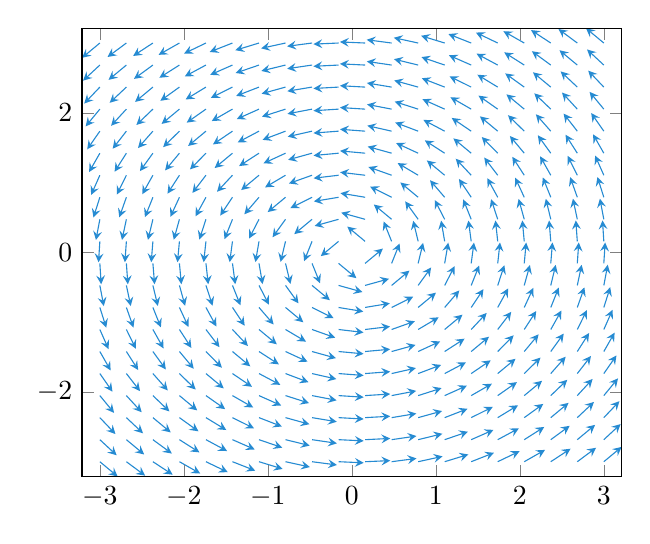
\begin{tikzpicture}
            \def\length{.5*sqrt(x^2+y^2)}
            \begin{axis}[domain=-3:3, view={0}{90}]
                \addplot3[blue, quiver={u={-y/(\length)}, v={x/(\length)}, scale arrows=0.15}, -stealth,samples=20] {0};
            \end{axis}
        \end{tikzpicture}
        \caption{
            \(
            \begin{bmatrix}
                \frac{-y}{\sqrt{x^2+y^2}} & \frac{x}{\sqrt{x^2+y^2}}
            \end{bmatrix}
            \)
        }\label{subfig:vecfield1}
    \end{subfigure}
    \vskip\baselineskip
    \begin{subfigure}[b]{\subfigwidth}
        \centering
        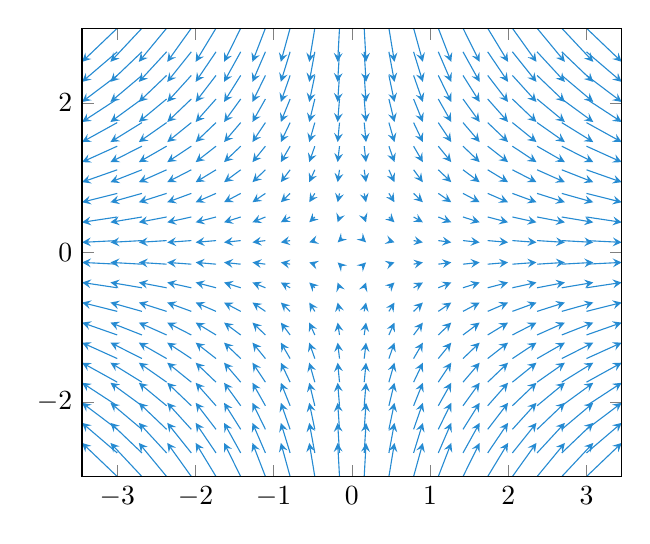
\begin{tikzpicture}
            \begin{axis}[domain=-3:3, view={0}{90}]
                \addplot3[blue, quiver={u={x}, v={-y}, scale arrows=0.15}, -stealth,samples=20] {0};
            \end{axis}
        \end{tikzpicture}
        \caption{
            \(
            \begin{bmatrix}
                x & y
            \end{bmatrix}
            \)
        }\label{subfig:vecfield2}
    \end{subfigure}
    \caption{Vector fields.}\label{fig:vectorfields}
\end{figure}
%</vecfields>

%<*coordinatechart>
\begin{figure*}
    \newcommand*{\scale}{1.5}
    \centering
    \begin{tikzpicture}[thick,scale=\scale, every node/.style={scale=\scale}]
        \path[->] (0.8, 0) edge [bend right] node[left, xshift=-2mm] {$\phi_i$} (-1, -2.9);
        \draw[white,fill=white] (0.06,-0.57) circle (.15cm);
        \path[->] (-0.7, -3.05) edge [bend right] node [right, yshift=-3mm] {$\phi^{-1}$} (1.093, -0.11);
        \draw[white, fill=white] (0.95,-1.2) circle (.15cm);

        % Functions j
        \path[->] (5.8, -2.8) edge [bend left] node[midway, xshift=-5mm, yshift=-3mm] {$\psi^{-1}$} (3.8, -0.35);
        \draw[white, fill=white] (4,-1.1) circle (.15cm);
        \path[->] (4.2, 0) edge [bend left] node[right, xshift=2mm] {$\psi$} (6.2, -2.8);
        \draw[white, fill=white] (4.54,-0.12) circle (.15cm);

        % Manifold
        \draw[smooth cycle, tension=0.4, fill=white, pattern color=brown, pattern=north west lines, opacity=0.7] plot coordinates{(2,2) (-0.5,0) (3,-2) (5,1)} node at (3,2.3) {$M$};

        % Help lines
        %\draw[help lines] (-3,-6) grid (8,6);

        % Subsets
        \draw[smooth cycle, pattern color=orange, pattern=crosshatch dots]
        plot coordinates {(1,0) (1.5, 1.2) (2.5,1.3) (2.6, 0.4)}
        node [label={[label distance=-0.3cm, xshift=-2cm, fill=white]:$U$}] {};
        \draw[smooth cycle, pattern color=blue, pattern=crosshatch dots]
        plot coordinates {(4, 0) (3.7, 0.8) (3.0, 1.2) (2.5, 1.2) (2.2, 0.8) (2.3, 0.5) (2.6, 0.3) (3.5, 0.0)}
        node [label={[label distance=-0.8cm, xshift=.75cm, yshift=1cm, fill=white]:$V$}] {};

        % First Axis
        \draw[thick, ->] (-3,-5) -- (0, -5) node [label=above:$\phi(U)$] {};
        \draw[thick, ->] (-3,-5) -- (-3, -2) node [label=right:$\mathbb{R}^n$] {};

        % Arrow from i to j
        \draw[->] (0, -3.85) -- node[midway, above]{$\psi \circ \phi^{-1}$} (4.5, -3.85);
        \draw[<-] (0,-4.05) -- node[midway, below]{$\phi \circ \psi^{-1}$} (4.5, -4.05);

        % Second Axis
        \draw[thick, ->] (5, -5) -- (8, -5) node [label=above:$\psi(V)$] {};
        \draw[thick, ->] (5, -5) -- (5, -2) node [label=right:$\mathbb{R}^n$] {};

        % Sets in R^m
        \draw[white, pattern color=orange, pattern=crosshatch dots] (-0.67, -3.06) -- +(180:0.8) arc (180:270:0.8);
        \fill[even odd rule, white] [smooth cycle] plot coordinates{(-2, -4.5) (-2, -3.2) (-0.8, -3.2) (-0.8, -4.5)} (-0.67, -3.06) -- +(180:0.8) arc (180:270:0.8);
        \draw[smooth cycle] plot coordinates{(-2, -4.5) (-2, -3.2) (-0.8, -3.2) (-0.8, -4.5)};
        \draw (-1.45, -3.06) arc (180:270:0.8);

        \draw[white, pattern color=blue, pattern=crosshatch dots] (5.7, -3.06) -- +(-90:0.8) arc (-90:0:0.8);
        \fill[even odd rule, white] [smooth cycle] plot coordinates{(7, -4.5) (7, -3.2) (5.8, -3.2) (5.8, -4.5)} (5.7, -3.06) -- +(-90:0.8) arc (-90:0:0.8);
        \draw[smooth cycle] plot coordinates{(7, -4.5) (7, -3.2) (5.8, -3.2) (5.8, -4.5)};
        \draw (5.69, -3.85) arc (-90:0:0.8);
    \end{tikzpicture}
    \caption{Compatible coordinate charts.}\label{fig:compatcoordcharts}
\end{figure*}
%</coordinatechart>

%<*circlatlas>
\begin{figure*}
    \centering
    \includegraphics[width=\textwidth]{figures/chartsoncircle.png}
    \caption{Atlas of charts on the circle.}\label{fig:chartsoncircle}
\end{figure*}
%</circlatlas>
%<*chartsoncirc>
\begin{figure}
    \centering
    \includegraphics[width=\linewidth]{figures/xychartsoncircle.png}
    \caption{Atlas of charts on the circle.}\label{fig:xychartsoncircle}
\end{figure}
%</chartsoncirc>

%<*smoothatapoint>
\begin{figure}
    \centering
    \includegraphics[width=\linewidth]{figures/smoothatapoint.png}
    \caption{Smooth at a point.}\label{fig:smoothatapoint}
\end{figure}
%</smoothatapoint>

%<*smoothf>
\begin{figure}
    \centering
    \includegraphics[width=\textwidth]{figures/smoothF.png}
    \caption{Smooth at a point.}\label{fig:smoothf}
\end{figure}
%</smoothf>

%<*curvevec>
\begin{figure*}
    \centering
    \includegraphics[width=\linewidth]{figures/curvevector.png}
    \caption{Existence of a curve through a point with a given initial vector.}\label{fig:curvevec}
\end{figure*}
%</curvevec>

%<*smoothsec>
\begin{figure}
    \centering
    \includegraphics[width=\linewidth]{figures/smoothsection.png}
    \caption{A section of a vector bundle.}\label{fig:smoothsec}
\end{figure}
%</smoothsec>

%<*tangentbundle>
\begin{figure}
    \centering
    \includegraphics[width=\linewidth]{figures/tangentbundle.png}
    \caption{Tangent bundle to \(S^1\).}\label{fig:tangentbundle}
\end{figure}
%</tangentbundle>

%<*vecfield>
\begin{figure}
    \centering
    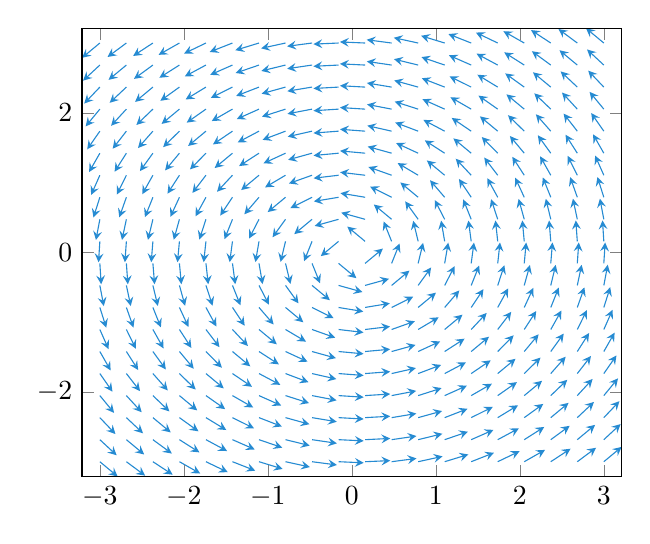
\begin{tikzpicture}
        \def\length{.5*sqrt(x^2+y^2)}
        \begin{axis}[domain=-3:3, view={0}{90}]
            \addplot3[blue, quiver={u={-y/(\length)}, v={x/(\length)}, scale arrows=0.15}, -stealth,samples=20] {0};
        \end{axis}
    \end{tikzpicture}
    \caption{Vector field \(X_{(x,y)} = \frac{1}{\sqrt{x^2+y^2}} \left( -y \pdv{x} + x \pdv{y} \right)\)}\label{fig:vecfield}
\end{figure}
%</vecfield>

%<*bumpfunction>
\begin{figure}
    \centering
    \includegraphics[width=\linewidth]{figures/bumpfunction.png}
    \caption{A bump function at 0 on \(\R\)}\label{fig:bumpfunction}
\end{figure}
%</bumpfunction>

%<*bumpfunction2>
\begin{figure}
    \centering
    \includegraphics[width=\linewidth]{figures/bumpfunction2.png}
    \caption{A bump function at 0 on \(\R\)}\label{fig:bumpfunction2}
\end{figure}
%</bumpfunction2>

%<*localflow>
\begin{figure}
    \centering
    \includegraphics[width=\linewidth]{figures/localflow.png}
    \caption{The flow line through \(q\) of a local flow}\label{fig:localflow}
\end{figure}
%</localflow>

%<*liederivative>
\begin{figure}
    \centering
    \includegraphics[width=\linewidth]{figures/liederivative.png}
    \caption{Comparing the values of \(Y\) at nearby points.}\label{fig:liederivative}
\end{figure}
%</liederivative>

%<*mobius>
\begin{figure}
    \centering
    \newcommand*{\subfigwidth}{\linewidth}
    \begin{subfigure}[b]{\subfigwidth}
        \centering
        \includegraphics[width=\linewidth]{figures/mobius.png}
        \caption{M{\"o}bius band}\label{subfig:mobius}
    \end{subfigure}

    \begin{subfigure}[b]{\subfigwidth}
        \centering
        \includegraphics[width=\textwidth]{figures/orientmobius.png}
        \caption{Non-orientability of the M{\"o}bius band}\label{subfig:orientmobius}
    \end{subfigure}
    \caption{}\label{fig:orientations}
\end{figure}
%</mobius>

%<*sphericalcoordinates>
\begin{figure}
    \centering
    \newcommand*{\subfigwidth}{\linewidth}
    \begin{subfigure}[b]{\subfigwidth}
        \centering
        \includegraphics[width=\textwidth]{figures/sphericalcoordinates.png}
        \caption{Spherical coordinates in \(\R^3\)}\label{subfig:sphericalcoordinates}
    \end{subfigure}
    \vskip\baselineskip
    \begin{subfigure}[b]{\subfigwidth}
        \centering
        \includegraphics[width=\textwidth]{figures/paramspherical.png}
        \caption{A parameterization by spherical coordinates}\label{subfig:paramspherical}
    \end{subfigure}
    \caption{}\label{fig:spherical}
\end{figure}
%</sphericalcoordinates>
\localtableofcontents

Artificial Neural Network (ANN or simply NN) algorithms for SR are all based on a Convolutional Neural Network (CNN) architecture.
%
We first, briefly, review ANNs in general, CNNs in particular, powerful architectures called Deep Neural Networks (DNNs), and a training methodology for networks called Generative Adversarial Networks (GANs).
%
We then proceed to review applications of ANNs to super resolution.
%
\subsection{Basics}
\begin{figure*}
    % MLP
    \centering
    \tikzstyle{inputNode}=[draw,fill=sail,circle,minimum size=10pt,inner sep=2pt]
    \tikzstyle{hiddenNode}=[draw,fill=snowymint,circle,minimum size=10pt,inner sep=2pt]
    \tikzstyle{outputNode}=[draw,fill=plum,circle,minimum size=10pt,inner sep=2pt]
    \tikzstyle{stateTransition}=[-stealth, thick]
    \begin{subfigure}[b]{0.49\textwidth}
        \centering
        \begin{tikzpicture}
            \node[draw,fill=plum, circle,minimum size=25pt,inner sep=0pt] (x) at (0,0) {$\Sigma$ $\sigma$};
            \draw[dashed] (0,-0.43) -- (0,0.43);

            \node[inputNode] (x0) at (-2, 1.5) {$ x_1$};
            \node[inputNode] (x1) at (-2, 0.75) {$ x_2$};
            \node[inputNode] (x2) at (-2, 0) {$ x_3$};
            \node[inputNode] (x3) at (-2, -0.75) {$ x_4$};
            \node[inputNode] (xn) at (-2, -1.95) {$ x_n$};

            \draw[stateTransition] (x0) to[out=0,in=120] node [midway, sloped, above] {$w_1$} (x);
            \draw[stateTransition] (x1) to[out=0,in=150] node [midway, sloped, above] {$w_2$} (x);
            \draw[stateTransition] (x2) to[out=0,in=180] node [midway, sloped, above] {$w_3$} (x);
            \draw[stateTransition] (x3) to[out=0,in=210] node [midway, sloped, above] {$w_4$} (x);
            \draw[stateTransition] (xn) to[out=0,in=240] node [midway, sloped, above] {$w_n$} (x);
            \draw[stateTransition] (x) -- (4,0) node [midway,above] {$z(\mathbf{x}) = \sigma\left(\sum\limits_{i=1}^{n}{w_ix_i} +  b\right)$};
            \node (dots) at (-2, -1.25) {$\vdots$};
        \end{tikzpicture}
        \caption{Single Artificial Neuron function.}\label{fig:singleann}
    \end{subfigure}
    \begin{subfigure}[b]{0.49\textwidth}
        \centering
        \begin{tikzpicture}

            \node[inputNode, thick] (i1) at (6, 0.75) {$x_1$};
            \node[inputNode, thick] (i2) at (6, 0) {$x_2$};
            \node[] (i4) at (6, -0.75) {$\LARGE \vdots$};
            \node[inputNode, thick] (i3) at (6, -1.5) {$x_n$};

            \node[hiddenNode, thick] (h1) at (8, 1.5) {$z_1$};
            \node[hiddenNode, thick] (h2) at (8, 0.75) {$z_2$};
            \node[hiddenNode, thick] (h3) at (8, 0) {$z_3$};
            \node[] (h4) at (8, -0.75) {$\LARGE \vdots$};
            \node[]  at (8, -1.5) {$\LARGE \vdots$};
            \node[hiddenNode, thick] (h5) at (8, -2.25) {$z_m$};

            \node[outputNode, thick] (o2) at (10, 0) {$\Sigma$ $\sigma$};
            \draw[dashed] (10,-0.43) -- (10,0.43);

            \draw[stateTransition] (i1) -- (h1);
            \draw[stateTransition] (i1) -- (h2);
            \draw[stateTransition] (i1) -- (h3);
            \draw[stateTransition] (i1) -- (h5);
            \draw[stateTransition] (i2) -- (h1);
            \draw[stateTransition] (i2) -- (h2);
            \draw[stateTransition] (i2) -- (h3);
            \draw[stateTransition] (i2) -- (h5);
            \draw[stateTransition] (i3) -- (h1);
            \draw[stateTransition] (i3) -- (h2);
            \draw[stateTransition] (i3) -- (h3);
            \draw[stateTransition] (i3) -- (h5);

            \draw[stateTransition] (h1) -- (o2);
            \draw[stateTransition] (h2) -- (o2);
            \draw[stateTransition] (h3) -- (o2);
            \draw[stateTransition] (h5) -- (o2);

            \node[above=of i1, align=center] (l1) {\footnotesize $n$ Neuron \\ \footnotesize Input \\ \footnotesize layer};
            \node[right=1.3em of l1, align=center] (l2) {\footnotesize $m$ Neuron \\ \footnotesize Hidden \\ \footnotesize layer};
            \node[right=2.3em of l2, align=center] (l3) {\footnotesize Output \\ \footnotesize layer};

            \draw[stateTransition] (o2) -- node[midway,above] {$y(\mathbf{x}) = \sigma'\left(\sum\limits_{j=1}^{m}{w'_jz_j} + b'\right)$} (13, 0);
        \end{tikzpicture}
        \caption{Multi-layer ANN.}\label{fig:multiann}
    \end{subfigure}
    \caption{Artificial Neural Network representation.}\label{fig:ann}
\end{figure*}

An ANN is a function specified by composing elementary functions called \newterm{artificial neurons}\anote{ann} (or simply neurons).
%
Neurons consist of a set of inputs \(\mathbf{x} \coloneqq (x_1, x_2, \dots, x_n)\), a set of parameters called weights \(w_i\), and an \newterm{activation function} \(\sigma\), which acts as a thresholding mechanism.
%
For example, the simplest function that qualifies as a neuron is a linear function:
\begin{equation}
    z(\mathbf{x}) = w_1 x_1 + w_2 x_2 = \sum_i w_i x_i
    \label{eqn:simpleann}
\end{equation}
where the activation function is the trivial one the identity.
%
Common non-trivial activation functions are the sigmoid function
\begin{equation}
    \operatorname{sig}(x)={\frac {1}{1+e^{-x}}}={\frac {e^{x}}{e^{x}+1}}
\end{equation}
the hyperbolic tangent function
\begin{equation}
    \tanh x={\frac {\sinh x}{\cosh x}}={\frac {e^{x}-e^{-x}}{e^{x}+e^{-x}}}={\frac {e^{2x}-1}{e^{2x}+1}}
\end{equation}
and the piecewise defined \newterm{rectified linear unit} (\(\operatorname{ReLU}\)):
\begin{align}
    \operatorname{ReLU}(x) & \coloneqq \begin{cases}x&{\text{if }}x>0,\\0&{\text{otherwise}}\end{cases} 
                        %    & = \max(0, x)
\end{align}
Note that eqn.~\eqref{eqn:simpleann} passes through the origin \((0,0,0)\) since it has no constant term; in the parlance of machine learning (ML) the neuron is missing a bias term\anote{bias} \(b\):
\begin{equation}
    z(\mathbf{x}) = \sum_i w_i x_i + b
    \label{eqn:linearregr}
\end{equation}

Neurons can be represented as directed graphs, where a vertex represents an input and edges represent the weights (see figure~\ref{fig:singleann}).
%
ANNs are, then, assemblies of neurons grouped into \newterm{layers} with the layers composed by applying neurons to outputs from immediately preceding layers.
%
For example the ANN specified in figure~\ref{fig:multiann} represents the function
\begin{equation}
    \begin{split}
        y(\mathbf{x}) &= \sigma' \left( \sum_j w'_j z_j(\mathbf{x}) + b' \right) \\
        &=  \sigma' \left( \sum_{j=1}^m w'_j \sigma\left(\sum_{i=1}^n w_i x_i + b_j\right) + b' \right)
    \end{split}
\end{equation}
%
Layers are categorized as either \newterm{hidden layers} or input-output layers: those layers that are not input or output layers are hidden layers.

ANNs seem like a very simple class of functions; for example, Minsky \etal \cite{minsky2017perceptrons} famously proved that single-layer ANNs that don't include a nonlinear activation function can't represent \(\operatorname{XOR}\)\anote{xor}. 
%
On the contrary, strikingly, ANNs that do include a nonlinear activation function satisfy a \newterm{universal approximation theorem} \cite{cybenko1989approximation}:
%
given any continuous function \(f\) (on some bounded interval \(I\)) there exists a sequence of ANNs (with at least one hidden layer and employing a nonlinear activation function) whose limit approximates\anote{uniformconv} \(f\) to arbitrary precision.

A critical component of the universal approximation theorem is finding the correct sequence of ANNs; in the parlance of ML an ANN demands a \newterm{learning rule}.
%
In general, ANN learning rules iterate on the weights \(w_i\) given \(k \gg 1\) \newterm{training} pairs of known \newterm{samples} and \newterm{targets} \(\left\{ \bm{x}_k, t_k \right\}\) of \(f\). 
%
The most common such learning rule is a \newterm{gradient descent} based rule called the Delta rule \cite{widrow1960adaptive}.
%
It is derived from minimizing the \(L_2\) loss with respect to each of the weights using gradient descent:
\begin{equation}
    L(w_1, \dots, w_n) \coloneqq \sum_k \frac{1}{2} (t_k - y(\mathbf{x}_k))^2
    \label{eqn:loss}
\end{equation}
and hence
\begin{equation}
    \pd{L}{w_i} = - \sum_k(t_k-y(\bm{x}_k))\cdot y'\cdot x_{ik}
\end{equation}
where by \(y' \coloneqq \sigma'\) we mean the derivative of the activation function with respect to its argument and by \(x_{ik}\) we mean the \(i\)-th input \(x_i\) of the \(k\)-th training sample \(\bm{x}_k\).
%
Hence, by gradient descent, the weights \(w_i\) should be adjusted in the opposite direction of \(\pd{L}{w_i}\) and we have the weight update rule
\begin{equation}
    \Delta w_i \coloneqq \alpha \cdot \sum_k(t_k-y(\mathbf{x}_k))\cdot \sigma'\cdot x_{ik}
    \label{eqn:batchupdate}
\end{equation}
where \(\alpha\) is a small constant called the \newterm{learning rate} (that controls the rate of convergence of the ANN).

In general, deriving the partial derivatives \(\pd{L}{w_i}\) for a multi-layer, wide (many neurons in each layer) network is compute intensive due to dependencies between weights in adjacent layers.
%
\begin{figure}[!htbp]
    \centering
    \begin{subfigure}[b]{.49\textwidth}
        \centering
        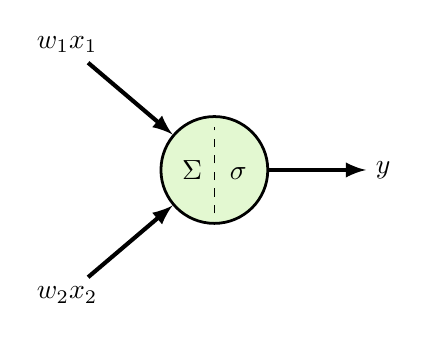
\begin{tikzpicture}[]
            \def\pindist{35pt}
            \def\nodesize{38pt}

            \tikzstyle{every pin edge}=[signal]
            \tikzstyle{annot} = [text width=4em, text centered]

            \node[hiddennode, text width=\nodesize, minimum size=\nodesize,
                pin={[pin edge={latex-}, pin distance=\pindist]above left:$w_1 x_1$},
                pin={[pin edge={latex-}, pin distance=\pindist]below left:$w_2 x_2$},
                pin={[pin edge={-latex}, pin distance=\pindist]right:$y$}
            ] (N1) at (-100pt,0) {$\Sigma\quad \sigma$};
            \draw[dashed] (-100pt,-0.55) -- (-100pt,0.55);
        \end{tikzpicture}
        \caption{Forward Pass.}
    \end{subfigure}
    \vskip\baselineskip
    \begin{subfigure}[b]{.49\textwidth}
        \centering
        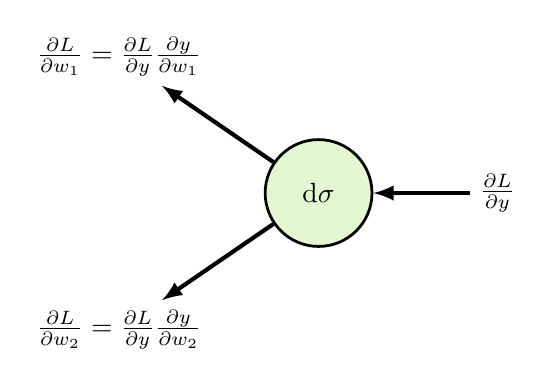
\begin{tikzpicture}[]
            \def\pindist{35pt}
            \def\nodesize{38pt}
            \tikzstyle{every pin edge}=[signal]
            \tikzstyle{annot} = [text width=4em, text centered]

            \node[hiddennode, text width=\nodesize, minimum size=\nodesize,
                pin={[pin edge={-latex}, pin distance=\pindist]above left:$\frac{\partial L}{\partial w_1}=\frac{\partial L}{\partial y}\frac{\partial y}{\partial w_1}$},
                pin={[pin edge={-latex}, pin distance=\pindist]below left:$\frac{\partial L}{\partial w_2}=\frac{\partial L}{\partial y}\frac{\partial y}{\partial w_2}$},
                pin={[pin edge={latex-}, pin distance=\pindist]right:$\frac{\partial L}{\partial y}$}
            ] (N2) at (+120pt,0) {$\dif \sigma$};
        \end{tikzpicture}
        \caption{Backwards Pass. Note that \(\pd{L}{y}\) can be reused when computing both \(\pd{L}{w_1}\) and \(\pd{L}{w_2}\).}
    \end{subfigure}
    \caption{Back-propagation computation of derivatives.}\label{fig:backprop}
\end{figure}

Fortunately traversing the derivative-dependency graph in a particular order, a technique called \newterm{back-propagation}\anote{backprop} or simply backprop (see figure~\ref{fig:backprop}), makes this tractable.

Another inefficiency of the Delta rule is that it requires evaluating the ANN on the entire set of samples in order to compute the update \(\Delta w_i\).
%
For large training sets (on the order of millions of samples) this is infeasible due to memory limitations.
%
Stochastic Gradient Descent (SGD) replaces computing the total loss in eqn.~\eqref{eqn:batchupdate} with computing a partial loss called the \newterm{batch loss}:
\begin{equation}
    \Delta w_i^t = w_i^t - w_i^{t-1} \coloneqq \alpha \cdot \sum_j (t_j-y(\mathbf{x}_j))\cdot \sigma'\cdot x_{ij}
    \label{eqn:sgd}
\end{equation}
where the sum on the right-hand side is now over a subset of samples called a \newterm{batch}.
%
This in effect computes the weight update \(\Delta w_i\) incrementally and saves having to hold all training data in memory concurrently.
%
The disadvantage of using SGD is that the batch loss is a noisy estimate of the total loss; in order to assure convergence one typically trains and retrains ANNs on random shufflings of the training data.
%
Each such training episode is called an \newterm{epoch}.
%
% Equation~\eqref{eqn:sgd} is evaluated for each of the \(k\) samples sequentially and therefore saves having to store all training samples in memory.





\subsubsection{Convolutional Neural Networks}




The one-dimensional (1D) discrete convolution \((f*g)\) of 1D discrete functions \(f,g\) is defined
\begin{equation}
    (f*g)[n]\coloneqq \sum _{i} f[i]g[n-i]
    \label{eqn:1dconv}
\end{equation}
The convolution of a function \(f\) with a finite sequence of values \(g\) can be interpreted as filtering \(f\) with the filter \(g\); for example convolving a noisy \(f\) with a Heaviside function smoothes \(f\) (see figure~\ref{fig:convfiltering}).
\begin{figure}[!htbp]
    \centering
    \begin{subfigure}[b]{.49\textwidth}
        \centering
        \includegraphics[width=0.95\textwidth]{figures/neural_networks/unsmoothed.png}
        \caption{Noisy function \(f\) (Gaussian process sample).}\label{fig:convnoisy}
    \end{subfigure}

    \begin{subfigure}[b]{.49\textwidth}
        \centering
        \includegraphics[width=0.95\textwidth]{figures/neural_networks/kernel.png}
        \caption{Heaviside function (low-pass filter \(g\)).}\label{fig:convfilter}
    \end{subfigure}
    \begin{subfigure}[b]{.49\textwidth}
        \centering
        \includegraphics[width=0.95\textwidth]{figures/neural_networks/smoothed.png}
        \caption{Smoothed (low-pass filtered) \(f * g\).}\label{fig:convsmooth}
    \end{subfigure}
    \caption{Convolution as filtering.}\label{fig:convfiltering}
\end{figure}
%
The sequence of values that comprise \(g\) is called the \newterm{kernel} of the \(g\) and the length of the sequence is called the \newterm{bandwidth} of the kernel (or simply width).
%
The two-dimensional (2D) discrete convolution \((f*g)\) of 2D discrete functions \(f,g\) is defined
\begin{equation}
    (f*g)[n, m]\coloneqq \sum _{i}\sum _{j}f[i, j]g[n-i, m-j]
    \label{eqn:2dconv}
\end{equation}
and can be interpreted in exactly the same way as 1D convolutions.
%
For 2D convolutions the kernels are most often square and therefore the kernel dimensions are specified rather than just width (see figure~\ref{fig:2dconv}).
\begin{figure*}
    \centering

    \tikzset{
        inputsquare/.pic={
                \draw[fill=sail] (0,0) rectangle (4,4);
                \draw[black, thick] (0,0) grid (4,4);
                \node at (0.5,0.5) {2};
                \node at (0.5,1.5) {3};
                \node at (0.5,2.5) {0};
                \node at (0.5,3.5) {3};
                \node at (1.5,0.5) {2};
                \node at (1.5,1.5) {1};
                \node at (1.5,2.5) {0};
                \node at (1.5,3.5) {3};
                \node at (2.5,0.5) {3};
                \node at (2.5,1.5) {3};
                \node at (2.5,2.5) {0};
                \node at (2.5,3.5) {2};
                \node at (3.5,0.5) {2};
                \node at (3.5,1.5) {1};
                \node at (3.5,2.5) {1};
                \node at (3.5,3.5) {1};
            },
        pics/filtersquare/.style args={#1/#2/#3/#4}{
                code = {
                        \draw[fill=snowymint] (#1,#2) rectangle (#3,#4);
                        \draw[black, thick] (#1,#2) grid (#3,#4);
                        \node at (#1+0.5,#2+0.5) {0};
                        \node at (#1+0.5,#2+1.5) {2};
                        \node at (#1+0.5,#2+2.5) {0};
                        \node at (#1+1.5,#2+0.5) {0};
                        \node at (#1+1.5,#2+1.5) {2};
                        \node at (#1+1.5,#2+2.5) {0};
                        \node at (#1+2.5,#2+0.5) {1};
                        \node at (#1+2.5,#2+1.5) {0};
                        \node at (#1+2.5,#2+2.5) {2};
                    }},
        pics/outputsquare/.style args={#1/#2/#3/#4}{
                code = {
                        \draw[fill=plum] (0,0) rectangle (2,2);
                        \draw[black, thick] (0,0) grid (2,2);
                        \node at (0.5,0.5) {#3};
                        \node at (0.5,1.5) {#1};
                        \node at (1.5,0.5) {#4};
                        \node at (1.5,1.5) {#2};
                    }}
    }
    \newcommand*{\figwidth}{.25}
    \newcommand*{\figscale}{1}
    \begin{subfigure}[b]{\textwidth}
        \centering
        \begin{tikzpicture}[scale=1,every node/.style={minimum size=1cm},on grid]
            \node (node) at (-0.5,2) {$f = $};
            \pic {inputsquare};
            \begin{scope}[xshift=5cm, yshift=0.5cm]
                \node (node) at (-0.5,1.5) {$g = $};
                \pic {filtersquare=0/0/3/3};
            \end{scope}
            \begin{scope}[xshift=9.5cm, yshift=1cm]
                \node (node) at (-0.75,1) {$f * g = $};
                \pic {outputsquare=7/3/11/12};
            \end{scope}
        \end{tikzpicture}
        \caption{Input \(f\), 2-D \(3 \times 3\) convolution kernel \(g\), and output \(f * g\).}
    \end{subfigure}
    \vskip\baselineskip
    \begin{subfigure}[b]{\textwidth}
        \centering
        \begin{tikzpicture}[scale=\figscale,every node/.style={minimum size=1cm},on grid]
            \begin{scope}[every node/.append style={yslant=0.5,xslant=-0.7},
                    yslant=0.5,xslant=-0.7]

                \pic {inputsquare};
                \coordinate (BL) at (0,1);
                \coordinate (BR) at (3,1);
                \coordinate (TL) at (0,4);
                \coordinate (TR) at (3,4);
            \end{scope}
            \begin{scope}[
                    xshift=-.4,
                    yshift=.4cm,
                    every node/.append style={yslant=0.5,xslant=-0.7,opacity=.4},
                    yslant=0.5,xslant=-0.7]
                \pic{filtersquare=0/1/3/4};

                \coordinate (EBL) at (0,1);
                \coordinate (EBR) at (3,1);
                \coordinate (ETL) at (0,4);
                \coordinate (ETR) at (3,4);

            \end{scope}
            \begin{scope}[xshift=-5, yshift=5cm,
                    every node/.append style={yslant=0.5,xslant=-0.7},
                    yslant=0.5,xslant=-0.7]

                \draw (EBL) -- (0,1) (EBR) -- (1,1)
                (ETL) -- (0,2)    (ETR) -- (1,2);

                \draw (EBL) -- (BL) (EBR) -- (BR)
                (ETL) -- (TL)     (ETR) -- (TR);

                \pic{outputsquare=7/0/0/0};
            \draw[fill=black, opacity=0.3] (0,1) rectangle (1,2);

            \end{scope}
        \end{tikzpicture}
        \begin{tikzpicture}[scale=\figscale,every node/.style={minimum size=1cm},on grid]
            \begin{scope}[every node/.append style={yslant=0.5,xslant=-0.7},
                    yslant=0.5,xslant=-0.7]
                \pic{inputsquare};
                \coordinate (BL) at (1,1);
                \coordinate (BR) at (4,1);
                \coordinate (TL) at (1,4);
                \coordinate (TR) at (4,4);
            \end{scope}
            \begin{scope}[
                    xshift=-.4,
                    yshift=.4cm,
                    every node/.append style={yslant=0.5,xslant=-0.7,opacity=.4},
                    yslant=0.5,xslant=-0.7]

                \pic{filtersquare=1/1/4/4};

                \coordinate (EBL) at (1,1);
                \coordinate (EBR) at (4,1);
                \coordinate (ETL) at (1,4);
                \coordinate (ETR) at (4,4);
            \end{scope}
            \begin{scope}[xshift=-5, yshift=5cm,
                    every node/.append style={yslant=0.5,xslant=-0.7},
                    yslant=0.5,xslant=-0.7]
                \draw (EBL) -- (1,1) (EBR) -- (2,1)
                (ETL) -- (1,2)    (ETR) -- (2,2);
                \draw (EBL) -- (BL) (EBR) -- (BR)
                (ETL) -- (TL)    (ETR) -- (TR);

                \pic{outputsquare=7/3/0/0};
                \draw[fill=black, opacity=0.3] (1,1) rectangle (2,2);

            \end{scope}
        \end{tikzpicture}

        \begin{tikzpicture}[scale=\figscale,every node/.style={minimum size=1cm},on grid]
            \begin{scope}[every node/.append style={yslant=0.5,xslant=-0.7},
                    yslant=0.5,xslant=-0.7]
                \pic{inputsquare};
                \coordinate (BL) at (0,0);
                \coordinate (BR) at (3,0);
                \coordinate (TL) at (0,3);
                \coordinate (TR) at (3,3);
            \end{scope}
            \begin{scope}[
                    xshift=-.4,
                    yshift=.4cm,
                    every node/.append style={yslant=0.5,xslant=-0.7,opacity=.4},
                    yslant=0.5,xslant=-0.7]
                \pic{filtersquare=0/0/3/3};

                \coordinate (EBL) at (0,0);
                \coordinate (EBR) at (3,0);
                \coordinate (ETL) at (0,3);
                \coordinate (ETR) at (3,3);
            \end{scope}
            \begin{scope}[xshift=-5, yshift=5cm,
                    every node/.append style={yslant=0.5,xslant=-0.7},
                    yslant=0.5,xslant=-0.7]
                \draw (EBL) -- (0,0) (EBR) -- (1,0)
                (ETL) -- (0,1)    (ETR) -- (1,1);
                \draw (EBL) -- (BL) (EBR) -- (BR)
                (ETL) -- (TL)    (ETR) -- (TR);

                \pic{outputsquare=7/3/11/0};
                \draw[fill=black, opacity=0.3] (0,0) rectangle
                (1,1);

            \end{scope}
        \end{tikzpicture}
        \begin{tikzpicture}[scale=\figscale,every node/.style={minimum size=1cm},on grid]
            \begin{scope}[every node/.append style={yslant=0.5,xslant=-0.7},
                    yslant=0.5,xslant=-0.7]
                \pic{inputsquare};

                \coordinate (BL) at (1,0);
                \coordinate (BR) at (4,0);
                \coordinate (TL) at (1,3);
                \coordinate (TR) at (4,3);
            \end{scope}
            \begin{scope}[
                    xshift=-.4,
                    yshift=.4cm,
                    every node/.append style={yslant=0.5,xslant=-0.7,opacity=.4},
                    yslant=0.5,xslant=-0.7]
                \pic{filtersquare=1/0/4/3};
                \coordinate (EBL) at (1,0);
                \coordinate (EBR) at (4,0);
                \coordinate (ETL) at (1,3);
                \coordinate (ETR) at (4,3);
            \end{scope}
            \begin{scope}[xshift=-5, yshift=5cm,
                    every node/.append style={yslant=0.5,xslant=-0.7},
                    yslant=0.5,xslant=-0.7]
                \draw (EBL) -- (1,0) (EBR) -- (2,0)
                (ETL) -- (1,1)    (ETR) -- (2,1);
                \draw (EBL) -- (BL) (EBR) -- (BR)
                (ETL) -- (TL)    (ETR) -- (TR);
                \pic{outputsquare=7/3/11/12};
                \draw[fill=black, opacity=0.3] (1,0) rectangle (2,1);

            \end{scope}
        \end{tikzpicture}
        \caption{Evaluation of convolution.}\label{fig:2dconviter}
    \end{subfigure}
    \caption{2-D convolution.}\label{fig:2dconv}
\end{figure*}

Notice that eqns.~\eqref{eqn:1dconv} and~\eqref{eqn:2dconv} are completely linear in their inputs \(f[i]\) (\(f[i,j]\)) with weights \(w_i = g[n-i]\) (\(w_{ij} = g[n-i, m-j]\)) and hence naturally constitute a neuron (layer of neurons); a \newterm{convolution layer} in a multi-layer ANN is either eqn.~\eqref{eqn:1dconv} or eqn.~\eqref{eqn:2dconv} with kernel values being iteratively updated by the learning rule.
%
Hence, a CNN is an ANN with one or more convolution layers; CNNs consisting of 2D convolutions are particularly effective for tasks that operate on images (since image patches have more structure than image slices).

In practice multiple filters are applied to the same input and then stacked to produce a higher-dimensional output (see figure~\ref{fig:multconvs}), each dimension of which is called a \newterm{feature map}.
\begin{figure}[!htbp]
    \centering
    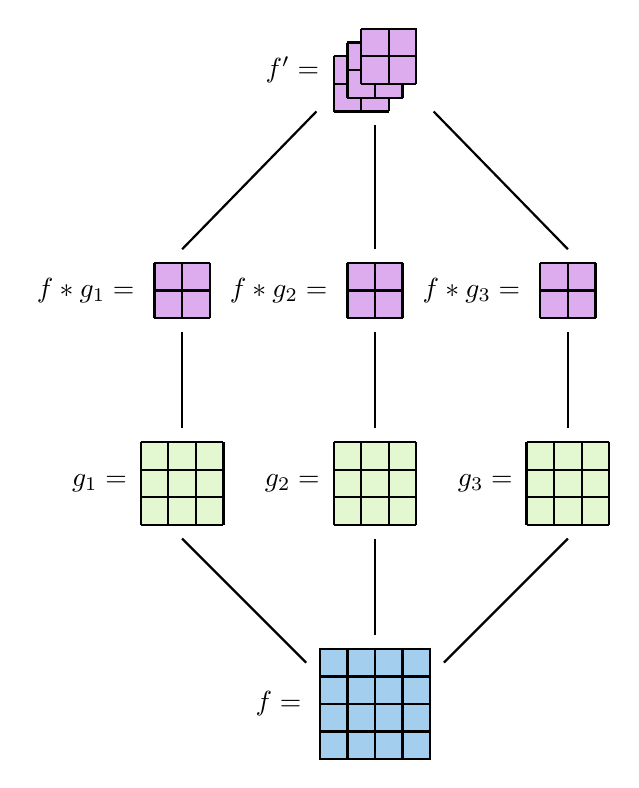
\begin{tikzpicture}[scale=.35,every node/.style={minimum size=1cm}, on grid]
        \begin{scope}[]
            \node (node) at (-1.5,2) {$f = $};
            \draw[fill=sail,thick]
            (0,0) grid (4,4) rectangle (0,0);
        \end{scope}

        \foreach \x [count=\i] in {-7,0,7} {%
                \begin{scope}[xshift=\x cm,yshift=8cm]
                    \begin{scope}[xshift=0.5cm,yshift=0.5cm]
                        \node (node) at (-1.5,1.5) {$g_\i = $};
                        \draw[fill=snowymint] (0,0) rectangle (3,3);
                        \draw[black, thick] (0,0) grid (3,3);
                    \end{scope}
                \end{scope}
                \begin{scope}[xshift=\x cm,yshift=16cm]
                    \begin{scope}[xshift=1cm]
                        \node (node) at (-2.5,1) {$f * g_\i = $};
                        \draw[fill=plum] (0,0) rectangle (2,2);
                        \draw[black, thick] (0,0) grid (2,2);
                    \end{scope}
                \end{scope}
            }
        \begin{scope}[xshift=1cm,yshift=24cm]
            \node (node) at (-2,1) {$f' = $};
            \foreach \s in {-0.5,0, 0.5} {%
                    \begin{scope}[xshift=\s cm,yshift=\s cm]
                        \draw[fill=plum] (0,0) rectangle (2,2);
                        \draw[black, thick] (0,0) grid (2,2);
                    \end{scope}
                }
        \end{scope}
        \draw[thick] (-0.5,3.5)   -- (-5,8);
        \draw[thick] (2,4.5)      -- (2,8) ;
        \draw[thick] (4.5,3.5)    -- (9,8) ;

        \draw[thick] (-5,12) -- (-5,15.5);
        \draw[thick] (2,12) -- (2,15.5)  ;
        \draw[thick] (9,12) -- (9,15.5)  ;

        \draw[thick] (-5,18.5) --(-0.125,23.5);
        \draw[thick] (2,18.5) -- (2,23)   ;
        \draw[thick] (9,18.5) -- (4.125,23.5) ;
    \end{tikzpicture}
    \caption{A convolution layer consisting of three distinct \(3\times 3\) filters.}\label{fig:multconvs}
\end{figure}
%
Depending on whether the CNN is being employed to solve a generative task or a classification task the activation function might be either a \(\operatorname{ReLU}\) (applied element-wise to the output of the convolution layer) or a \newterm{max-pooling} filter:
\begin{multline}
    \operatorname{max-pool}(f,g)[n, m]\coloneqq\\ \max_{i,j}\left[ f[i, j]g[n-i, m-j] \right]
    \label{eqn:2dpool}
\end{multline}
There are many other convolution operators (e.g., strided, dilated, transposed) that are beyond the scope of this survey \cite{dumoulin2016guide}.





\subsubsection{Deep Neural Networks}\label{subsubsec:dnns}





%
Deep Neural Networks (DNNs) are ANNs that have multiple layers and many neurons in each layer.
%
Intuitively the advantage of deep networks (over shallow networks) is they learn\anote{learn} hierarchies of concepts (called \newterm{features}); for example in facial recognition tasks, layers proximal to the input layer learn to recognize elementary features such as edges, layers distal to the input layer learn abstractions of elementary features, such as arrangements of edges that comprise eyes or noses, and layers even more distal to the input layer learn entire faces.

Training DNNs presents many challenges; due to their depth they suffer from issues such as \newterm{vanishing gradients} and \newterm{overfitting}.
%
Vanishing gradients is an all but complete cessation of substantive updates to weights; consider the partial derivative of the activation function \(\sigma'\) in eqn.~\eqref{eqn:batchupdate}.
%
Notice that if \(\abs{\sigma'} \ll 1\) then \(\Delta w_i\) will be very small.
%
This occurs for a single neuron when the input \newterm{saturates} the activation function; for example for \(\operatorname{sig}\) this happens when \(\abs{x} > 5\) because the gradient \(\sigma'\) is very small (see figure~\ref{fig:activs}).
\begin{figure}[!htbp]
    \centering
    \includegraphics[width=\linewidth]{figures/neural_networks/activation_grads.png}
    \caption[]{Sigmoid activation gradients. Note that for \(\abs{x} > 5\) the gradient is almost 0.}\label{fig:activs}
\end{figure}
%
For multi-layer ANNs, such as DNNs, even if no single neuron saturates the activation function,
due to the chain rule, weight updates for layers near the input are proportional to very many factors that are less than one (whose product therefore is near 0).
%
Overfitting, on the other hand, can be interpreted as memorization of the training samples; since the minimization problem (eqn.~\eqref{eqn:loss}) that leads to the Delta rule only measures \(\abs{t_k - y(\mathbf{x}_k)}\), DNNs can simply encode responses to many (or most) of the training samples in their weights (in order to effectively minimize). 
%
This is possible due to DNNs having so many degrees of freedom\anote{largeparams}.

\begin{figure}
    \centering
    \begin{subfigure}[c]{0.49\textwidth}
        \centering
        \includegraphics[width=\textwidth, trim=145 50 145 0, clip]{figures/neural_networks/batch_norm.png}
        \caption[]{Batch normalization's effect, for a single neuron, on inputs to a Sigmoid activation function.}\label{fig:batchnorm1}
    \end{subfigure}

    \begin{subfigure}[b]{0.49\textwidth}
        \centering
        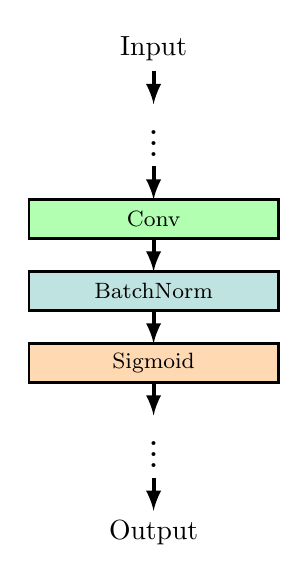
\begin{tikzpicture}[
            start chain=going below, node distance=12pt,
            point/.append style={on chain, join=by {signal}},
            layer/.append style={on chain, join=by {signal}},
        ]
        \node[point] {Input};
        \node[point] {$\LARGE \vdots$};
        \node[conv] {Conv};
        \node[bn] {BatchNorm};
        \node[activation] {Sigmoid};
        \node[point] {$\LARGE \vdots$};
        \node[point] {Output};
    \end{tikzpicture}
    \caption[]{Batch normalization as a layer in a DNN.}\label{fig:batchnorm2}
    \end{subfigure}
    \caption[]{Batch normalization.}\label{fig:batchnorm}
\end{figure}
\begin{figure*}[!htbp]
    \centering
    \begin{adjustbox}{center}
        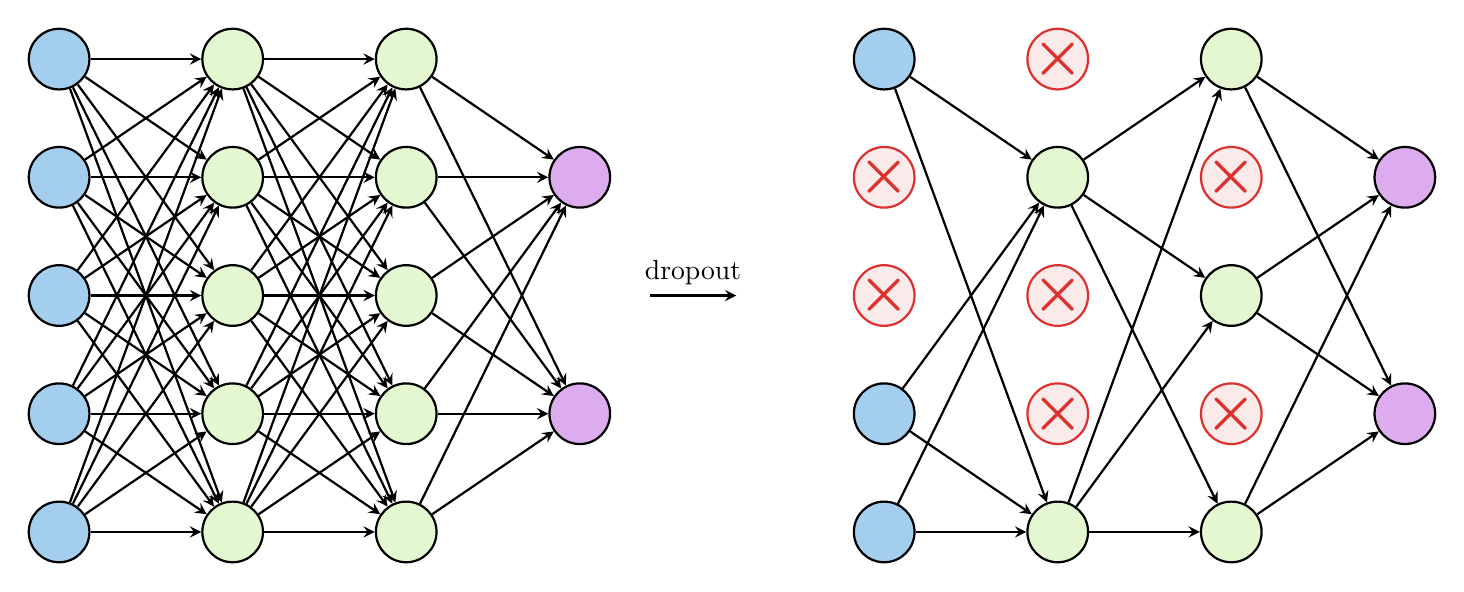
\begin{tikzpicture}
            \node[inputnode, circle, draw, thick] (i1) {};
            \node[inputnode, circle, draw, thick, above=2em of i1] (i2) {};
            \node[inputnode, circle, draw, thick, above=2em of i2] (i3) {};
            \node[inputnode, circle, draw, thick, below=2em of i1] (i4) {};
            \node[inputnode, circle, draw, thick, below=2em of i4] (i5) {};

            \node[hiddennode, circle, draw, thick, right=4em of i1] (h1) {};
            \node[hiddennode, circle, draw, thick, right=4em of i2] (h2) {};
            \node[hiddennode, circle, draw, thick, right=4em of i3] (h3) {};
            \node[hiddennode, circle, draw, thick, right=4em of i4] (h4) {};
            \node[hiddennode, circle, draw, thick, right=4em of i5] (h5) {};

            \node[hiddennode, circle, draw, thick, right=4em of h1] (hh1) {};
            \node[hiddennode, circle, draw, thick, right=4em of h2] (hh2) {};
            \node[hiddennode, circle, draw, thick, right=4em of h3] (hh3) {};
            \node[hiddennode, circle, draw, thick, right=4em of h4] (hh4) {};
            \node[hiddennode, circle, draw, thick, right=4em of h5] (hh5) {};

            \node[outputnode, circle, draw, thick, right=4em of hh2] (o1) {};
            \node[outputnode, circle, draw, thick, right=4em of hh4] (o2) {};

            \draw[-stealth, thick] (i1) -- (h1);
            \draw[-stealth, thick] (i1) -- (h2);
            \draw[-stealth, thick] (i1) -- (h3);
            \draw[-stealth, thick] (i1) -- (h4);
            \draw[-stealth, thick] (i1) -- (h5);
            \draw[-stealth, thick] (i2) -- (h1);
            \draw[-stealth, thick] (i2) -- (h2);
            \draw[-stealth, thick] (i2) -- (h3);
            \draw[-stealth, thick] (i2) -- (h4);
            \draw[-stealth, thick] (i2) -- (h5);
            \draw[-stealth, thick] (i3) -- (h1);
            \draw[-stealth, thick] (i3) -- (h2);
            \draw[-stealth, thick] (i3) -- (h3);
            \draw[-stealth, thick] (i3) -- (h4);
            \draw[-stealth, thick] (i3) -- (h5);
            \draw[-stealth, thick] (i4) -- (h1);
            \draw[-stealth, thick] (i4) -- (h2);
            \draw[-stealth, thick] (i4) -- (h3);
            \draw[-stealth, thick] (i4) -- (h4);
            \draw[-stealth, thick] (i4) -- (h5);
            \draw[-stealth, thick] (i5) -- (h1);
            \draw[-stealth, thick] (i5) -- (h2);
            \draw[-stealth, thick] (i5) -- (h3);
            \draw[-stealth, thick] (i5) -- (h4);
            \draw[-stealth, thick] (i5) -- (h5);

            \draw[-stealth, thick] (h1) -- (hh1);
            \draw[-stealth, thick] (h1) -- (hh2);
            \draw[-stealth, thick] (h1) -- (hh3);
            \draw[-stealth, thick] (h1) -- (hh4);
            \draw[-stealth, thick] (h1) -- (hh5);
            \draw[-stealth, thick] (h2) -- (hh1);
            \draw[-stealth, thick] (h2) -- (hh2);
            \draw[-stealth, thick] (h2) -- (hh3);
            \draw[-stealth, thick] (h2) -- (hh4);
            \draw[-stealth, thick] (h2) -- (hh5);
            \draw[-stealth, thick] (h3) -- (hh1);
            \draw[-stealth, thick] (h3) -- (hh2);
            \draw[-stealth, thick] (h3) -- (hh3);
            \draw[-stealth, thick] (h3) -- (hh4);
            \draw[-stealth, thick] (h3) -- (hh5);
            \draw[-stealth, thick] (h4) -- (hh1);
            \draw[-stealth, thick] (h4) -- (hh2);
            \draw[-stealth, thick] (h4) -- (hh3);
            \draw[-stealth, thick] (h4) -- (hh4);
            \draw[-stealth, thick] (h4) -- (hh5);
            \draw[-stealth, thick] (h5) -- (hh1);
            \draw[-stealth, thick] (h5) -- (hh2);
            \draw[-stealth, thick] (h5) -- (hh3);
            \draw[-stealth, thick] (h5) -- (hh4);
            \draw[-stealth, thick] (h5) -- (hh5);


            \draw[-stealth, thick] (hh1) -- (o1);
            \draw[-stealth, thick] (hh1) -- (o2);
            \draw[-stealth, thick] (hh2) -- (o1);
            \draw[-stealth, thick] (hh2) -- (o2);
            \draw[-stealth, thick] (hh3) -- (o1);
            \draw[-stealth, thick] (hh3) -- (o2);
            \draw[-stealth, thick] (hh4) -- (o1);
            \draw[-stealth, thick] (hh4) -- (o2);
            \draw[-stealth, thick] (hh5) -- (o1);
            \draw[-stealth, thick] (hh5) -- (o2);
            \draw[-stealth, thick] (7.5,0) -- node[above] {dropout} (8.6, 0);
            %%% BOUNDARY %%%
            \node[inputnode, circle, draw, thick, red, fill=red!10, right=15em of hh1] (i1) {};
            \node[inputnode, circle, draw, thick, red, fill=red!10, above=2em of i1] (i2) {};
            \node[inputnode, circle, draw, thick, above=2em of i2] (i3) {};
            \node[inputnode, circle, draw, thick, below=2em of i1] (i4) {};
            \node[inputnode, circle, draw, thick, below=2em of i4] (i5) {};

            \node[red] (icr) at (i1) {$\mathlarger{\mathlarger{\mathlarger{\mathlarger{\mathlarger{\bm{\times}}}}}}$};
            \node[red] (icr) at (i2) {$\mathlarger{\mathlarger{\mathlarger{\mathlarger{\mathlarger{\bm{\times}}}}}}$};

            \node[hiddennode, circle, draw, thick, red, fill=red!10, right=4em of i1] (h1) {};
            \node[hiddennode, circle, draw, thick, right=4em of i2] (h2) {};
            \node[hiddennode, circle, draw, thick, red, fill=red!10, right=4em of i3] (h3) {};
            \node[hiddennode, circle, draw, thick, red, fill=red!10, right=4em of i4] (h4) {};
            \node[hiddennode, circle, draw, thick, right=4em of i5] (h5) {};

            \node[red] (icr) at (h1) {$\mathlarger{\mathlarger{\mathlarger{\mathlarger{\mathlarger{\bm{\times}}}}}}$};
            \node[red] (icr) at (h3) {$\mathlarger{\mathlarger{\mathlarger{\mathlarger{\mathlarger{\bm{\times}}}}}}$};
            \node[red] (icr) at (h4) {$\mathlarger{\mathlarger{\mathlarger{\mathlarger{\mathlarger{\bm{\times}}}}}}$};

            \node[hiddennode, circle, draw, thick, right=4em of h1] (hh1) {};
            \node[hiddennode, circle, draw, thick, red, fill=red!10, right=4em of h2] (hh2) {};
            \node[hiddennode, circle, draw, thick, right=4em of h3] (hh3) {};
            \node[hiddennode, circle, draw, thick, red, fill=red!10, right=4em of h4] (hh4) {};
            \node[hiddennode, circle, draw, thick, right=4em of h5] (hh5) {};

            \node[red] (icr) at (hh2) {$\mathlarger{\mathlarger{\mathlarger{\mathlarger{\mathlarger{\bm{\times}}}}}}$};
            \node[red] (icr) at (hh4) {$\mathlarger{\mathlarger{\mathlarger{\mathlarger{\mathlarger{\bm{\times}}}}}}$};

            \node[outputnode, circle, draw, thick, right=4em of hh2] (o1) {};
            \node[outputnode, circle, draw, thick, right=4em of hh4] (o2) {};

            \draw[-stealth, thick] (i3) -- (h2);
            \draw[-stealth, thick] (i3) -- (h5);
            \draw[-stealth, thick] (i4) -- (h2);
            \draw[-stealth, thick] (i4) -- (h5);
            \draw[-stealth, thick] (i5) -- (h2);
            \draw[-stealth, thick] (i5) -- (h5);

            \draw[-stealth, thick] (h2) -- (hh1);
            \draw[-stealth, thick] (h2) -- (hh3);
            \draw[-stealth, thick] (h2) -- (hh5);
            \draw[-stealth, thick] (h5) -- (hh1);
            \draw[-stealth, thick] (h5) -- (hh3);
            \draw[-stealth, thick] (h5) -- (hh5);

            \draw[-stealth, thick] (hh1) -- (o1);
            \draw[-stealth, thick] (hh1) -- (o2);
            \draw[-stealth, thick] (hh3) -- (o1);
            \draw[-stealth, thick] (hh3) -- (o2);
            \draw[-stealth, thick] (hh5) -- (o1);
            \draw[-stealth, thick] (hh5) -- (o2);
        \end{tikzpicture}
    \end{adjustbox}
    \caption[]{Dropout regularization technique. Note that approximately only \(50\%\) of the neurons are active.}\label{fig:dropout}
\end{figure*}
Overfitting and vanishing gradients are only two of the challenges in training sophisticated ANNs.
%
Fortunately there exist a set of practices, called Deep Learning, that make training DNNs feasible.
%
For example, to combat vanishing gradient, Batch Normalization \cite{ioffe2015batch} is used to normalize outputs from linear layers prior to activation (see figure~\ref{fig:batchnorm}).
%
This centering and scaling of the data ensures that no single neuron will saturate its activation function.
%
It operates on a batch by batch basis, \((0,1)-\)Normal normalizing inputs to each layer's activation function:
\begin{align}
    \bm{\mu} _{B}        & \coloneqq {\frac {1}{m}}\sum _{j=1}^{m}\bm{x}_{j}                                             \\
    \bm{\sigma} _{B}^{2} & \coloneqq{\frac {1}{m}}\sum _{j=1}^{m}(\bm{x}_{j}-\bm{\mu}_{B})^{2}                           \\
    {\hat {\bm{x}}}      & \coloneqq {\frac {\bm{x}-\bm{\mu}_{B}}{\sqrt {\bm{\sigma}_{B}^{2}}}} \label{eqn:bathcnormdiv}
\end{align}
where \(m\) is the batch size and the operations in eqn.~\eqref{eqn:bathcnormdiv} are understood to be broadcast (i.e., \(\sqrt {\bm{\sigma} _{B}^{2}}\) is an element-wise root and elements of \(\sqrt {\bm{\sigma} _{B}^{2}}\) divide corresponding elements of \(\bm{x}-\bm{\mu}_{B}\)).
%
In fact Batch normalization actually has two parameters \(\gamma, \beta\) that it learns (using backprop) from the data: the output \(\bm{y}\) after batch normalization is actually defined
\begin{equation}
    \bm{y} \coloneqq \gamma \bm{\hat{x}} + \beta 
\end{equation}
The intuitive reason for learning \(\beta, \gamma\) instead of just fixing them to be \(0,1\) is that \((0,1)\)-Normal normalization isn't necessarily correct in all cases (so why not learn the \((\beta,\gamma)\)-Normal normalization as informed by training data).
%
\begin{figure*}
	\begin{adjustbox}{width=\textwidth}
		% \begin{tikzpicture}

		% 	\node[circle, draw, thick] (z) {$\vec{z}$};
		% 	\node[circle, draw, thick, right=5em of z] (x) {$\vec{x}_{fake}$};
		% 	\draw[-stealth, thick] (z) -- node[above] {$G(\vec{z})$} node[below] {generator} (x);
		% 	\node[left=of z] (i) {};
		% 	\draw[-stealth, thick] (i) -- node[above] {$p_\theta(\vec{z})$} (z);
		% 	\node[above=of x, circle, draw, thick] (xt) {$\vec{x}_{real}$};
		% 	\node[left=5em of xt] (it) {};
		% 	\draw[-stealth, thick] (it) -- node[above] {$p_{data}(\vec{x})$} (xt);
		% 	\node[circle, draw, thick, right=5em of x, yshift=2.5em] (D) {$\vec{x}$};
		% 	\node[right=7em of D] (out) {real?};
		% 	\draw[-stealth, thick] (D) -- node[above] {$D(\vec{x})$} node[below] {discriminator} (out);

		% 	\node[right=2.5em of x, circle, fill, inner sep=0.15em] (pt1) {};
		% 	\node[right=2.5em of xt, circle, fill, inner sep=0.15em] (pt2) {};

		% 	\draw[dashed, thick] (pt1) edge[bend left] (pt2);

		% 	\node[circle, draw, thick, fill=white, inner sep=0.15em] at ([xshift=-0.9em, yshift=4em]pt1.north) (pt3) {};

		% 	\draw[-stealth, thick] (x) -- (pt1);
		% 	\draw[-stealth, thick] (xt) -- (pt2);
		% 	\draw[-stealth, thick] (pt3) -- (D);

		% \end{tikzpicture}
		\includegraphics[]{figures/neural_networks/gan.jpeg}
	\end{adjustbox}
	\caption{Schematic diagram for Generative Adversarial Network\cite{ponti2017}.}\label{fig:gan}

\end{figure*}

\begin{figure}
    \centering

        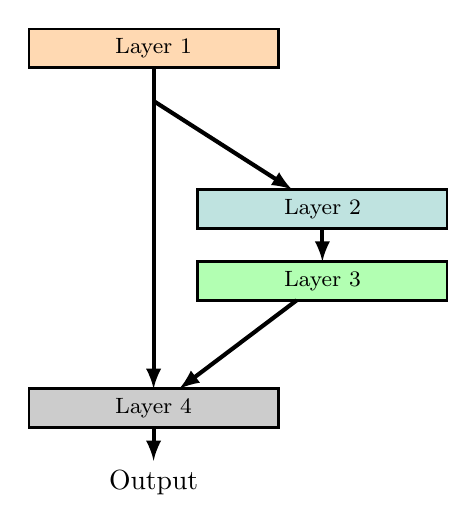
\begin{tikzpicture}[start chain=going below, node distance=12pt,
            point/.append style={on chain, join=by {signal}},
            layer/.append style={on chain, join=by {signal}},
            branch/.append style={on chain, join=by {signal, -}},
            ]
            \def\branchy{20pt}

            \node[activation] {Layer 1};
            \node[branch] (input) {};
            \node[bn, xshift=\layerwidth/2+16pt, yshift=-\branchy] {Layer 2};
            \node[conv] {Layer 3};
            \node[layer, xshift=-\layerwidth/2-16pt, yshift=-\branchy] (add) {Layer 4};
            \node[point] {Output};
            \draw[signal] (input) -- (add);
        \end{tikzpicture}
    \caption{Skip connection connecting non-adjacent layers.}\label{fig:skipconnection}
\end{figure}
Another solution to the vanishing gradients problem is using \newterm{skip connections}: outputs from a layer can be made to skip adjacent layers early on in training (see figure~\ref{fig:skipconnections}).
%
This has the effect that substantive gradients can be propagated farther back into the network during the initial part of training when weights should be changing the most (since they're ostensibly far from a minimum).

Overfitting in some sense is a problem opposite of vanishing gradients; while vanishing gradients prevent the DNN from learning, overfitting means the DNN is learning too easily.
%
Naturally then, overfitting is mitigated by using regularization; methods such as \(L_2\) regularization and \newterm{dropout} have been shown to be effective against overfitting \cite{bengio2013}.
%
\(L_2\) regularization incorporates a squared weight term \(\frac{\lambda}{2}\sum_{i=1}^n w_i^2\) into eqn.~\eqref{eqn:loss}, which translates into a \newterm{weight decay} term \(\lambda w_i^{t-1}\) in the Delta rule (eqn.~\eqref{eqn:sgd}):
\begin{equation}
    \Delta w_i^t = \alpha \cdot \sum_j (t_j-y(\mathbf{x}_j))\cdot \sigma'\cdot x_{ij} + \lambda w_i^{t-1}
    \label{eqn:weightdecaydelta}
\end{equation}
On the other hand dropout enforces regularization by selectively disabling neurons in the network (see figure~\ref{fig:dropout}); on each forward pass through the network a neuron is either passed input or not according to some probability \(p\) (usually \(p = 0.5\)).
%
The intuition being that not every neuron will have an opportunity to learn from every sample thereby limiting the capacity of the ANN to memorize patterns unique to the training samples.

There are many other best-practices techniques for training DNNs that are beyond the scope of this brief review; an accessible survey is Montavon \etal \cite{montavon2012neural}.




\subsubsection{Generative Adversarial Networks}\label{subsubsec:gan}




A Generative Adversarial Network \cite{goodfellow2014generative} is a training regimen for networks that perform \newterm{generative tasks}.
%
A generative task is one which calls for generating samples from a probability distribution represented by the training data.
%
For example one might have many images of people and one might wish to generate new samples (see figure~\ref{fig:stylegan}) from the probability distribution of such images (i.e., new images of people).
\begin{figure}[!htbp]
    \centering
    \begin{adjustbox}{width=\linewidth}
        \centering
        \includegraphics[]{figures/neural_networks/stylegan.jpg}
    \end{adjustbox}
    \caption{Uncurated set of images \textbf{generated} (i.e., none of the people depicted are real) using StyleGAN with the FFHQ dataset \cite{karras2018stylebased}.}\label{fig:stylegan}
\end{figure}
%
Super-resolution can be cast as a generative task: knowing the condtional distribution of high-frequency components in an image, one could recover said high-frequency components by drawing from that distribution.
%
In general, this is a highly non-trivial problem due to the dimensionality of the sample space.

GANs solve this problem by pitting a \newterm{generator} \(G\), that learns to transform samples from a readily available high-dimensional surrogate distribution (Normal or Uniform), against a \newterm{discriminator} \(D\).
The generator takes as input samples \(\bm{z}\) from the surrogate distribution \(p_{z}\) and outputs putative samples \(G(\bm{z})\) from the real distribution \(p_r\).
%
The discriminator alternates between considering true samples \(\bm{x}\) from the real distribution and considering counterfeit samples \(G(\bm{z})\) produced by the generator; it therefore assesses the quality of \(G\)'s output with respect to its own understanding of the real distribution.
%
To that end Goodfellow \etal \cite{goodfellow2014generative} propose a training framework that involves \(D\) and \(G \) playing a \newterm{mini-max game}\anote{minimax}:
\begin{equation}
    \min_G \max_D L(D, G)
\end{equation}
where
\begin{equation}
    L(D, G) \coloneqq \mathbb{E}_{\bm{x} \sim p_{r}} [\log D(\bm{x})] + \mathbb{E}_{\bm{z} \sim p_{z} } [\log(1 - D(G(\bm{z})))]
    \label{eqn:ganloss}
\end{equation}
Since the discriminator seeks to maximize \(L(D, G)\), the term \(\mathbb{E}_{\bm{x} \sim p_{r}} [\log D(\bm{x})]\) ensures that it is able to correctly identify (i.e., score high) true samples.
%
Simultaneously the term \(\mathbb{E}_{\bm{z} \sim p_{z} } [\log(1 - D(G(\bm{z})))] \) ensures that it is able to correctly identify (i.e., score low) counterfeit samples produced by \(G\).
%
Conversely, \(\mathbb{E}_{\bm{z} \sim p_{z} } [\log(1 - D(G(\bm{z})))]\) (the first term in eqn.~\eqref{eqn:ganloss}) does not play a role when optimizing \(G\)) and so \(G\) is encouraged to improve its ability to fool the discriminator (i.e., produce plausible samples from the real distribution).
%
Goodfellow \etal prove that for the generator this loss criterion is equivalent to minimizing the Jensen–Shannon divergence\anote{kldiv} between the distribution that it models and the true distribution of the data.
\subsection{Deep Neural Networks for SISR}
Deep neural network architectures for single-image super-resolution abide a four tiered hierarchy (according to complexity) which roughly parallels the chronological order of the innovations that have contributed to the current state of the art:
\begin{mdframed}
    \begin{itemize}
        \item \textbf{Pre-defined up-sampling}: networks that expect the image to already have been up-sampled (e.g., using bicubic interpolation). These networks chiefly restore high-frequency features that are omitted by the classical up-sampling technique.
        \item \textbf{Single up-sampling}: networks that perform the up-sampling themselves (in addition to performing restoration).
        \item \textbf{Progressive up-sampling}: networks that up-sample in phases, performing restoration at every phase.
        \item \textbf{Iterative up-sampling}: networks that up-sample and then assess the goodness of the result by down-sampling to original low-resolution (see section~\ref{subsubsec:iterback} for the classical analogue).
    \end{itemize}
\end{mdframed}



\subsubsection{SRCNN and Very Deep SR}\label{subsubsec:vdsr}




The first successful foray of Deep Learning into SISR was the 2-layer Super-Resolution CNN (SRCNN) model \cite{Dong_2016}.
%
SRCNN is a CNN composed of two convolution layers, with the first layer consisting of 64 filters (per color channel), the second layer consisting of 32 filters, and both layers employing \(\operatorname{ReLU}\) activations.
%
Dong \etal argue that their CNN architecture is equivalent to sparse coding SR (see figure~\ref{fig:srcnn}).
\begin{figure}[!htbp]
    \centering
    \newcommand*{\subfigwidth}{0.49\textwidth}
    \begin{subfigure}[b]{\subfigwidth}
        \includegraphics[width=\linewidth,keepaspectratio]{figures/neural_networks/sparse_coding.png}
        \caption{Sparse coding SR pipeline (see section~\ref{subsubsec:sparsecoding}).}\label{subfig:srcnnsparse}
    \end{subfigure}
    \vskip\baselineskip
    \begin{subfigure}[b]{\subfigwidth}
        \includegraphics[width=\linewidth,keepaspectratio]{figures/neural_networks/srcnn.png}
        \caption{SRCNN pipeline.}\label{subfig:srcnn}
    \end{subfigure}
    \caption{Sparse coding SR and SRCNN comparison \cite{Dong_2016}. Note both pipelines operate on bicubic up-sampled images.}\label{fig:srcnn}
\end{figure}
%
This is a common theme in the literature --- ANN architectures learning transformations equivalent to classical techniques --- owing to the universal approximation theorem.

Clearly, at least by modern standards, 2 layers isn't very deep; Dong \etal do experiment with an additional convolution layer but report difficulties maintaining reasonable convergence rates due to vanishing gradients.
%
Kim \etal \cite{Kim_2016} improve on SRCNN with Very Deep SRCNN (VDSR) by increasing the convolution layer count to a sum total of 20.
%
In order to overcome the training challenges faced by Dong \etal they use skip connections (see section~\ref{subsubsec:dnns}).
%
They also use learning rate \newterm{annealing}\anote{annealing} and implement gradient clipping to prevent \newterm{exploding gradients}\anote{gradclip}.
%
They further argue that an SR network need only learn \newterm{residuals} \(\bm{r} \coloneqq \bm{t} - \bm{x}\).
%
In this context, residuals have the significance of being the high-frequency components of an image, since the bicubic up-sampled input \(\bm{x}\) can be interpreted as a low-pass filtered version of the high-resolution image.
%
Hence, their loss function measures the error between the HR image target and the output of the network \(\bm{y}\) plus the input:
\begin{equation}
    L(\bm{t}, \bm{x}) \coloneqq \abs{\bm{t} - (\bm{x} + \bm{y})}^2
\end{equation}
where in the case that \(\bm{y}\) perfectly approximates \(\bm{r}\) the loss would be 0.




\subsubsection{Super-Resolution GAN}\label{subsubsec:srgan}




Single up-sampling networks forgo bicubic pre-processing and learn the up-sampling transformation as a component of the network.
%
The most interesting network in this class of networks is the Super-resolution Residual Network (SRResNet) along with its GAN trained counterpart SRGAN \cite{Ledig_2017}.
%
SRResNet takes as input LR images and similar to VDSR passes them through 16 individual ResBlocks (see figure~\ref{fig:resblock}) for feature extraction.
%
Where SRResNet differs from VDSR is the in-network up-sampling that it performs using \newterm{sub-pixel convolutions}.
%
Sub-pixel convolutions are a way to learn up-sampling as a component of the ANN.
%
They up-sample in two phases: first \(r^2\) filters are convolved with the input, where \(r\) is the up-sampling factor (e.g., 4 filters for 2x up-sampling), then a \newterm{pixel shuffle} operation reorders the elements of the feature maps into an \(r\)-times higher resolution grid (see figure~\ref{subfig:pixelshuffle}).
\begin{figure}[!htbp]
    \centering
    \newcommand*{\subfigwidth}{.49\textwidth}
    \begin{subfigure}[b]{\subfigwidth}
        \centering
        \includegraphics[width=\textwidth]{figures/neural_networks/subpixelconv1.png}
        \caption{Sub-pixel convolution as dilation then filtering.}\label{subfig:subpixdilate}
    \end{subfigure}
    \vskip\baselineskip
    \begin{subfigure}[b]{\subfigwidth}
        \centering
        \includegraphics[width=\textwidth]{figures/neural_networks/subpixelconv2.png}
        \caption{Sub-pixel convolution as filtering then pixel-shuffling.}\label{subfig:pixelshuffle}
    \end{subfigure}
    \caption{Sub-pixel convolution.}\label{fig:subpixelconv}
\end{figure}
%
This operation is called a sub-pixel convolution because it can be interpreted as first dilating the LR image and then convolving with a filter to get a feature map with sub-pixel (relative to the original LR image) responses (see figure~\ref{subfig:subpixdilate}).

Ledig \etal pre-train SRResNet using mean-squared-error (MSE) loss and then further train using the GAN framework (see section~\ref{subsubsec:gan}).
%
In addition to using the conventional GAN loss they add a term called \newterm{perceptual loss}:
\begin{equation}
    \ell_{feat}^{\phi, j} \left( \hat{\bm{y}}, \bm{y}_c\right) \coloneqq \frac{1}{H_j W_j} \abs{\phi_j\left({\hat{\bm{y}}}\right) - \phi_j \left(\bm{y}_c\right)}^2
\end{equation}
where \(\phi_j\) is the \(j\)-th layer activation of the VGG network \cite{simonyan2014very} pretrained on a large data set, \(\hat{\bm{y}}\) is the output of SRResNet, and \(\bm{y}_c\) is the target HR image (see figure~\ref{fig:perceptualloss}), and \(H_j, W_j\) are the dimensions of the \(j\)-th layer activation of VGG.
\begin{figure}[!htbp]
    \centering
    \begin{adjustbox}{width=\linewidth}
        \centering
        \includegraphics[]{figures/neural_networks/perceptual_loss.png}
    \end{adjustbox}
    \caption{Perceptual loss \cite{johnson2016perceptual}.}\label{fig:perceptualloss}
\end{figure}
%
They argue that this loss is closer to perceptual similarity than MSE loss and therefore encourages reconstruction of high frequency content that MSE loss alone omits.




\subsubsection{Laplacian Pyramid Super-Resolution Network}\label{subsubsec:lapsrn}




Lai \etal \cite{Lai_2017} propose a network that up-samples by predicting sub-band (see section~\ref{subsubsec:subband}) residuals at progressively finer and finer scales (i.e., higher and higher resolution).
%
Their network consists of \(\log_2(r)\), where \(r\) is the scaling factor, tiers of CNNs along two branches: a feature extraction branch and an image reconstruction branch (see figure~\ref{fig:lapsrn}).
\begin{figure}[!htbp]
    \centering
    \begin{adjustbox}{width=\linewidth}
        \centering
        \includegraphics{figures/neural_networks/lapsrn.png}
    \end{adjustbox}
    \caption{LapSRN architecture \cite{Lai_2017}.}\label{fig:lapsrn}
\end{figure}
\begin{figure}[!htbp]
    \centering
    \includegraphics[width=.4\textwidth]{figures/neural_networks/motion_compensation.png}
    \caption{Motion estimation module for BRCN \cite{caballero2017real}.}\label{fig:motion_estimation}
\end{figure}
%
For a given tier the feature extraction branch extracts the high-frequency components that comprise the residual and performs a 2x up-sampling (using transposed convolution). 
%
The output of the feature extraction branch, at a given tier, is then passed on to the next feature extraction tier and simultaneously to the corresponding image reconstruction tier.
%
The image reconstruction branch, at a given tier, up-samples the input image (also using transposed convolution) and element-wise sums it to the residual produced by the feature extraction branch (at the corresponding tier).
%
This structure emulates a Laplacian pyramid (see figure~\ref{fig:bertrand}) along both branches and as a result is called the Laplacian Pyramid Super-Resolution Network (LapSRN).

They also identify \(L_2\) loss as a source of perceptual fidelity flaws but unlike Ledig \etal they wholly substitute Charbonnier loss \cite{charbonnier1994two} \(\rho(\bm{x})\) to train their network:
\begin{equation}
    \rho(\bm{x}) \coloneqq \sqrt{\frac{\bm{x}\cdot \bm{x}}{\epsilon^2}+ 1}
\end{equation}
where \(\epsilon\) is a scale parameter that they empirically set to \(10^{-3}\). 
%
Lie \etal train their network using \newterm{deep supervision}; the loss function they optimize compares the result at every tier of the network against the target HR image (the HR image is down-sampled to produce targets at multiple scales):
\begin{equation}
    L(\bm{t}, \bm{y}) \coloneqq \sum_{i=1}^{\log_2(r)} \rho(\bm{t}_i - \bm{y}_i)
\end{equation}
where \(\bm{t}_i \coloneqq (t_{\log_2{(r)}}, \dots, t_1)\) is the target HR image down-sampled and \(\bm{y} \coloneqq (y_1, \dots, y_{\log_2(r)})\) are the outputs of LapSRN at each of the tiers.




\subsubsection{Deep Back-Projection Networks}\label{subsubsec:dbpn}




Inspired by recent theories on the function of the human visual cortex \cite{kravitz2013ventral} Harris \etal \cite{haris2018deep} propose a deep neural network for SR that incorporates error-correcting feedback mechanisms.
%
They build on the work of Irani \etal (see section~\ref{subsubsec:iterback}) and implement deep iterative back projections (DBPN) (see figure~\ref{fig:dbpn}).
\begin{figure*}[!htbp]
    \includegraphics[width=\textwidth,keepaspectratio]{figures/neural_networks/DBPN.png}
    \caption{End-to-end DBPN network.}\label{fig:dbpn}
\end{figure*}
%
These iterative back-projections are, in effect, repeated up-down-up sampling modules, implemented using skip connections and deconvolutions, that minimize reconstruction error (see figure~\ref{fig:updowndbpn}).
\begin{figure}[!htbp]
    \includegraphics[width=.49\textwidth,keepaspectratio]{figures/neural_networks/up_down_up.png}
    \caption{DBPN Up, Down projection unit components implementing error correction.}\label{fig:updowndbpn}
\end{figure}
%
In classical iterative back projection a sequence of LR images is used to estimate an HR image.
%
Harris \etal use only a single input LR image and produce multiple candidate HR images using multiple learned up-sampling operators.
%
Their Up-Projection module takes the error \(e_t^l\) between a proposed up-sampling \(H_0^t\) and the back-projection \(L_0^t\) and feeds it back into the proposed up-sampling, i.e., the error-correcting feedback is the difference between the back-projection and LR input.
%
Their Down-Projection module performs the same function but from HR to LR.
%
Using these modules they achieve state of the art up-sampling all the way up to 8x \cite{timofte2018ntire}.

\subsection{Deep Neural Networks for MISR}

MISR algorithms process a batch of LR images to generate a single HR image by aggregating non-redundant information across the LR images.
%
In order to effectively perform this task they must compensate for motion between the LR images by registering them to a common pixel grid (see section~\ref{sec:registration}).
%
In the context of neural networks this is framed as learning the time dependency from the training data (LR-HR image pair sequences) and then inferring such a time dependency for new samples.
%



\subsubsection{Bi-directional Recurrent CNN}




    \begin{figure*}[!htbp]
        \centering
        	\begin{adjustbox}{width=\textwidth}

        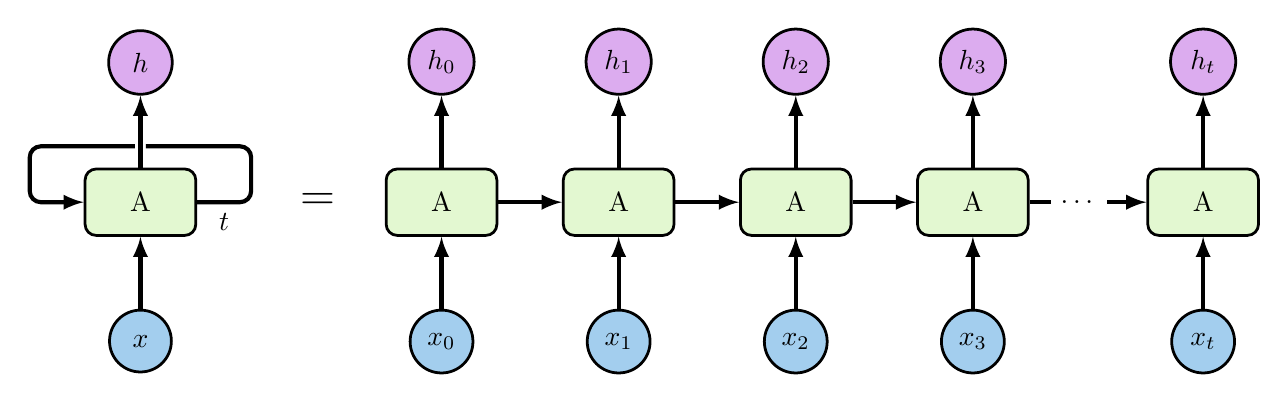
\begin{tikzpicture}
            \def\nodedist{64pt}

            \node[block, fill=snowymint, rounded corners, minimum width=40pt, minimum height=24pt] (at) at (0,0) {A};
            \node[inputnode, below=26pt of at] (xt) {$x$};
            \node[outputnode, above=26pt of at] (ht) {$h$};
            \draw[signal] (xt) -- (at);
            \draw[signal] (at) -- (ht);
            \coordinate (0t) at ($(ht)!0.6!(at)$);
            \draw[signal, -, shorten >=\intergape] (at) -- node[below] {$t$} +(40pt,0pt) |- (0t);
            \draw[signal, latex-, shorten >=\intergape] (at) -- +(-40pt,0pt) |- (0t);

            \newcommand{\timestep}[2]{
                \node[block, fill=snowymint, rounded corners, minimum width=40pt, minimum height=24pt] (a#2) at #1 {A};
                \node[inputnode, below=26pt of a#2] (x#2) {$x_#2$};
                \node[outputnode, above=26pt of a#2] (h#2) {$h_#2$};
                \draw[signal] (x#2) -- (a#2);
                \draw[signal] (a#2) -- (h#2);
            }

            % \timestep{(0, 0)}{t};

            \node[] (e) at ($(at) +(\nodedist,0)$) {\LARGE=};

            \timestep{($(e) +(0.7*\nodedist,0)$)}{0};
            \timestep{($(a0) +(\nodedist,0)$)}{1};
            \draw[signal] (a0) -- (a1);
            \timestep{($(a1) +(\nodedist,0)$)}{2};
            \draw[signal] (a1) -- (a2);
            \timestep{($(a2) +(\nodedist,0)$)}{3};
            \draw[signal] (a2) -- (a3);

            \node[] at ($(a3) +(0.6*\nodedist,0)$) (ddd) {$\dots$};
            \timestep{($(ddd) +(0.7*\nodedist,0)$)}{t};
            \draw[signal, -] (a3) -- (ddd);
            \draw[signal] (ddd) -- (at);
        \end{tikzpicture}
    \end{adjustbox}
    \caption{\(t\)-step RNN unrolled.}\label{fig:unrolledrnn}
    \end{figure*}
    % \begin{subfigure}[b]{.49\textwidth}
    %     \centering
    %     \begin{tikzpicture}[thick, node distance=30pt and 30pt, on grid]
    %         \node[cell, minimum width=200pt, minimum height=110pt, anchor=north west] (b) at (-2pt,0pt) {};

    %         \coordinate (cin) at (0pt,-20pt);
    %         \draw[signal] (cin) +(-\iolen, 0pt) node[above] {$c_{t-1}$} -- (cin);
    %         \coordinate (cout) at (200pt,-20pt);
    %         \draw[signal] (cout) -- +(\iolen,0pt) node[above left] {$c_{t}$};
    %         \coordinate (hin) at (0pt,-100pt);
    %         \draw[signal] (hin) +(-\iolen, 0pt) node[above] {$h_{t-1}$} -- (hin);
    %         \coordinate (hout) at (200pt,-100pt);
    %         \draw[signal] (hout) -- +(\iolen,0pt) node[above left] {$h_{t}$};
    %         \coordinate (h) at (184pt,0pt);
    %         \draw[signal] (h) -- +(0,\iolen) node[left] {$h_{t}$};
    %         \coordinate (x) at (14pt,-110pt);
    %         \draw[signal, -] (x) +(0pt,-\iolen) node[left] {$x_{t}$} -- (x);

    %         \node[celllayer] (f) at (32pt,-80pt) {$\operatorname{sig}$};
    %         \node[celllayer, right=34pt of f] (i) {$\operatorname{sig}$};
    %         \node[celllayer, right=34pt of i] (c) {$\tanh$};
    %         \node[celllayer, right=34pt of c] (o) {$\operatorname{sig}$};

    %         \node[pointwise, above=60pt of f] (fm) {$\times$};

    %         \node[pointwise, above=30pt of c] (cm) {$\times$};
    %         \node[pointwise, above=30pt of cm] (cmp) {$+$};

    %         \node[pointwise, above right=20pt and 20 pt of o] (om) {$\times$};
    %         \node[pointwise, above=20pt of om] (omt) {$\tanh$};

    %         \draw[signal] (f) edge node[near start,left] {$f_t$} (fm);

    %         \draw[signal, -] (c) edge node[pos=0.5,left] {$\tilde{c}_t$} (cm);
    %         \draw[signal] (cm) to (cmp);
    %         \draw[signal] (i) |- (cm) node[near start,left] {$i_t$};

    %         \draw[signal] (o) |- (om) node[pos=0.3,left] {$o_t$};

    %         \draw[signal, -] (fm) -- (cmp);

    %         \draw[signal, -] (cmp) -| (omt);
    %         \draw[signal, -] (omt) -- (om);

    %         \draw[signal] (cin) +(-\iolen, 0) node[above] {$c_{t-1}$} -- +(0,0);

    %         \draw[signal, -] (cin) +(-10pt,0) -- (fm);

    %         \draw[signal] (hin) +(-\iolen, 0) node[above] {$h_{t-1}$} -- +(0,0);

    %         \draw[signal, -] (hin) +(-10pt,0) -| (o);
    %         \draw[signal, -] (hin) -| (c);
    %         \draw[signal, -] (hin) -| (i);
    %         \draw[signal, -] (hin) -| (f);

    %         \draw[signal] (cout) -- +(\iolen,0) node[above left] {$c_{t}$};

    %         \draw[signal, -] (cmp) -- (cout);

    %         \draw[signal] (hout) -- +(\iolen,0) node[above left] {$h_{t}$};

    %         \draw[signal, -] (om) |- (hout);

    %         \draw[signal, -, shorten >=\intergape] (h |- hout) +(-10pt,0) -| (h |- cout);
    %         \draw[signal, shorten <=\intergape] (h |- cout) -- +(0,\iolen+20pt) node[left] {$h_{t}$};

    %         \draw[signal, -] (x) |- (f |- hin);
    %     \end{tikzpicture}
    %     \caption{Long Short Term Memory RNN unit.}\label{subfig:lstm}
    % \end{subfigure}

Huang \etal \cite{huang2015bidirectional} learn the time dependency for complex motions jointly with the up-sampling transformation using a Bidirectional Recurrent\anote{rnn} CNN (BRCN). 
%
% %
% That is to say, for a given \(t\) length sequence of data an RNN might respond differently than for a different \(t\) length sequence of data depending on the differing time dependencies intra-sequence.
%
They are able to model such non-stationary dependencies by using \newterm{loop unrolling} (see figure~\ref{fig:unrolledrnn}): a \(t\) length recursion is represented as \(t\) layers composed of \newterm{cells}.
%
It is these cells that keep track of the dependencies between elements of the sequences over arbitrary time intervals.
%
% As with all deep architectures RNN suffer from vanishing gradients; Long short-term memory (LSTM) cells address this problem by allowing gradients to flow through the cell unmediated (see figure~\ref{subfig:lstm}).
%
BRCN uses two recurrent networks, a forward-propagating network and a backward-propagating network.
%
Each of BRCN's RNNs is composed of two types of convolutions. 
%
The first are conventional (feed-forward) convolutions that model up-sampling.
%
The second, called recurrent and conditional convolutions, are convolutions in time that model time dependencies (see figure~\ref{fig:brcn}).
\begin{figure}[!htbp]
    \includegraphics[width=.49\textwidth]{figures/neural_networks/brcn.png}
    \caption{BRCN schematic diagram \cite{huang2015bidirectional}.}\label{fig:brcn}
\end{figure}
%
Note that the bi-directional framework incurs 3 image delay due the two hidden layers.
%
BRCN achieved (at the time) state of the art reconstruction performance for \(t=8\) image sequences but at \(\sim\)1s run-times it was far from real-time performance.




\subsubsection{Interlude: Attention and Spatial Transformers}\label{subsubsec:spatialtrans}


Attention mechanisms \cite{bahdanau2014neural} are neural network modules that can conditionally suppress certain parts of data (either at the input layer or at intermediate layers in the network).
%
Let \(\bm{x} \in \mathbb{R}^d\) be a sample and \(\bm{z} \in \mathbb{R}^k\) be the output at some intermediate layer.
%
Then \(f_\phi(\cdot) \in \left[0,1\right]^k\) is an attention network with learnable parameters \(\phi\), \(\bm{a} \coloneqq f_\phi (\bm{x})\) is an \newterm{attention vector}, and \(g = a \odot \bm{z}\) is an \newterm{attention glimpse} of \(\bm{z}\) (\(\odot\) is the Hadamard product).
%
As defined \(f_\phi\) is a \newterm{soft attention} mechanism; if \(f_\phi(\cdot) \in \left\{0,1\right\}^k\) (i.e., \(f_\phi\) learns a binary mask) then it is called a \newterm{hard attention} mechanism.
%
For example, \newterm{spatial attention} (attention applied to images) can be used to improve image captioning (see figure~\ref{fig:attention}).
\begin{figure*}[!htbp]
    \centering
    \includegraphics[width=\textwidth]{figures/neural_networks/attention.png}
    \caption[]{Attention for image captioning \cite{xu2015attend}.}\label{fig:attention}
\end{figure*}

A spatial transformer \cite{jaderberg2015spatial} is an attention mechanism that can also perform geometric transformations \(\mathcal{T}_{\bm{\theta}}\) of the data.
%
Note that the transformation is conditional on the input, just as attention is conditional on the input.
%
The transformer operates on input \(U\) to produce output \(V\) in three phases, each of which is implemented by a module (see figure~\ref{fig:spacetransformer}): 
%
\begin{figure}[!htbp]
    \centering
    \includegraphics[width=.49\textwidth]{figures/neural_networks/space_transformer.png}
    \caption{Spatial Transformer \cite{jaderberg2015spatial}.}\label{fig:spacetransformer}
\end{figure}
%
\begin{enumerate}
    \item \textbf{Localization}: a regression network \(f_{\text{loc}}(\cdot)\) that regresses the transformation parameters \(\bm{\theta}\) that parameterize the transformation \(\mathcal{T}_{\bm{\theta}}\). For example the six parameters that define an affine transformation (see figure~\ref{fig:affinetransformation}) in homogeneous coordinates.
    \item \textbf{Grid generation}: a sampling grid network, which generates the set of points where the input should be sampled to produce the transformed output (see figure~\ref{fig:paramsampling}). In practice it takes \(\bm{\theta}\) and the coordinate system as fixed parameters and generates a grid but in full generality this module can learn the correct coordinate representation.
    \item \textbf{Sampler}: a sampling kernel \(K\) that controls sampling strength on the transformed \((n,m)\) grid:
    \begin{equation*}
        V(x,y) = \sum_n \sum_m U(n,m) K(x-m, y-n)
    \end{equation*}
    Note that the kernel only need be a differentiable function such as, for example, the bilinear kernel \begin{equation*}
        K(i, j) \coloneqq \max(0, 1-\abs{i})\cdot \max(0, 1- \abs{j})
    \end{equation*}
\end{enumerate}
%
\begin{figure*}[!htbp]
    \centering
    \begin{subfigure}[b]{.39\textwidth}
        \centering
        \includegraphics[width=\textwidth]{figures/neural_networks/space_transformer_ti.png}
        \caption{Sampling grid \(G' = \mathcal{T}_I(G)\) where \(I\) is the identity transformation.}\label{subfig:spacetransformer_ti}
    \end{subfigure}
    \hspace{35pt}
    \begin{subfigure}[b]{.39\textwidth}
        \includegraphics[width=\textwidth]{figures/neural_networks/space_transformer_ttheta.png}
        \caption{Sampling grid \(G' = \mathcal{T}_{\bm{\theta}}(G)\) where \(\bm{\theta}\) defines a 2D affine transformation.}\label{subfig:spacetransformer_ttheta}
    \end{subfigure}
    \caption{parameterized sampling of image \(U\) to produce image \(V\) \cite{jaderberg2015spatial}.}\label{fig:paramsampling}
\end{figure*}


\subsubsection{Video Efficient Sub-Pixel Networks}



The first real-time DNN architecture (see figure~\ref{fig:realtimeepscn}) for MISR was based on a spatial transformer (see section~\ref{subsubsec:spatialtrans}) for motion compensation and efficient sub-pixel convolutions networks (ESPCN) for up-sampling (see section~\ref{subsubsec:srgan}).
\begin{figure*}[!htbp]
    \includegraphics[width=\textwidth]{figures/neural_networks/realtime_epscn.png}
    \caption{Real-time MISR with motion compensation \cite{caballero2017real}. Motion compensation is performed two adjacent frames in a triplet and all three frames are then passed to up-sampling network.}\label{fig:realtimeepscn}
\end{figure*}
%
In this use only the localization network of the spatial transformer is used to learn a pair of displacement mappings 
\begin{equation}
    \Delta_{t+1} \coloneqq (\Delta_{t+1}x, \Delta_{t+1} y)
\end{equation}
for each pixel in the images:
\begin{equation}
    \hat{\Delta} \coloneqq \underset{\Delta}{\text{argmin}}\left[\abs{I_t - I'_{t+1}}^2 + \lambda \mathcal{H}\left( \partial_{x,y} \Delta\right)\right]
\end{equation}
where the Huber loss \(\mathcal{H}\) is used as a regularizer (see section~\ref{subsubsec:huberloss}).
%
In fact the spatial transformer used by Caballero \etal estimates the optical flow in a course to fine fashion (see figure~\ref{fig:motionestimation}).
\begin{figure}
    \centering
    \includegraphics[width=.49\textwidth]{figures/neural_networks/motion_compensation.png}
    \caption{Coarse to fine flow estimation for ESCPN \cite{caballero2017real}}\label{fig:motionestimation}
\end{figure}


For the up-sampling itself Caballero \etal experiment with incorporating several sub-pixel convolution architectures that they call \newterm{fusion} methods.
%
Each fusion method applies convolutions to the sequence of images in either a tiered or conventional fashion (see figure~\ref{fig:fusions}) and then reorders the pixels to produce the HR image.
\begin{figure}[!htbp]
    \centering
    \newcommand*{\subfigwidth}{0.49\textwidth}
    \begin{subfigure}[b]{\subfigwidth}
        \centering
        \includegraphics[width=.7\linewidth,keepaspectratio]{figures/neural_networks/early_fusion.png}
        \caption{Early fusion.}\label{subfig:earlyfus}
    \end{subfigure}
    \vskip\baselineskip
    \begin{subfigure}[b]{\subfigwidth}
        \centering
        \includegraphics[width=\linewidth,keepaspectratio]{figures/neural_networks/slow_fusion.png}
        \caption{Slow fusion. If frames are processed in an online fashion then filter values should be shared. For example the last frame (purple) can recycle all of the computations above the dotted line.}\label{subfig:slowfus}
    \end{subfigure}
    % \vskip\baselineskip
    % \begin{subfigure}[b]{\subfigwidth}
    %     \includegraphics[width=\linewidth,keepaspectratio]{figures/neural_networks/3d_conv.png}
    %     \caption{3D convolution.}\label{subfig:updowndbpn}
    % \end{subfigure}
    \caption{Spatio-temporal ESPCN \cite{caballero2017real}.}\label{fig:fusions}
\end{figure}
%
For example, early fusion applies convolutions to a sequence of images as if they were independent channels of one image (see figure~\ref{subfig:earlyfus}).
%
Slow fusion, on the other hand, applies the convolutions in tiers in order to incorporate time dependencies in the filters (see figure~\ref{subfig:slowfus}).
%
Note that if adjacent filter banks are made to share weights then new incoming frames can recycle computations from earlier frames.




\subsubsection{Enhanced Deformable Convolutional Networks}



The current state-of-the-art DNN solution for MISR is the Enhanced Deformable Convolutional Network architecture (EDCN) \cite{wang2019edvr}.
%
This architecture consists of three (or four\anote{ntire}) independent stages implemented as self-contained modules (see figure~\ref{fig:edvr}): 
\begin{figure*}[!htbp]
    \includegraphics[width=\textwidth]{figures/neural_networks/edvr.png}
    \caption[]{Enhanced Deformable Convolutional Networks \cite{wang2019edvr}.}\label{fig:edvr}
\end{figure*}
\begin{mdframed}
    \begin{enumerate}
        \item \textbf{De-blur}: an optional pre-processing stage for deblurring images and potentially improving registration accuracy.
        \item \textbf{Registration}: an image registration stage effected by a Pyramid, Cascading and Deformable (PCD) alignment module.
        \item \textbf{Fusion}: a non-redundant information extraction stage effected by a Temporal and Spatial Attention (TSA) fusion module.
        \item \textbf{Reconstruction}: a high-frequency image artifact restoration stage effected by a cascade of ResBlocks (see section~\ref{subsubsec:vdsr}).
    \end{enumerate}
\end{mdframed}

The PCD alignment module uses tiered \newterm{deformable convolutions} in order to perform registration. 
%
A deformable convolution is a convolution with an irregularly shaped and spaced convolution kernel.
%
It is impelemented by learning the combination of a conventional kernel and an offset field that stores the offsets of each of the kernel values (see figure~\ref{fig:deformconv}).
\begin{figure}[!htbp]
    \centering
    \begin{subfigure}[b]{.49\textwidth}
        \centering
        \includegraphics[width=\textwidth]{figures/neural_networks/deformable_conv.png}
        \caption{Illustration of 3 \(\times\) 3 deformable convolution.}\label{subfig:deform_conv}
    \end{subfigure}
    \vskip\baselineskip
    \begin{subfigure}[b]{.49\textwidth}
        \centering
        \includegraphics[width=\textwidth]{figures/neural_networks/standard_deformable_conv.png}
        \caption{Standard vs. deformable convolution.}\label{subfig:deform_conv}
    \end{subfigure}
    \caption[]{Deformable convolutions \cite{Dai_2017}.}\label{fig:deformconv}
\end{figure}
%
For EDCN the deformable convolution deforms, with kernel \(w\), the input image \(I\) to an aligned image \(I'_t\) (relative to a reference image) according to 
\begin{equation}
    I'_t(\bm{x}) = \sum_{\bm{p}} w(\bm{p}) I_t(\bm{x} + \bm{p} + \Delta \bm{p})
\end{equation}
where \(\bm{p} \in \left\{(-1,-1), (-1, 0), \dots, (0,1), (1,1)\right\}\) and \(\Delta \bm{p}\) is the learned offset.

The TSA module \newterm{attends} in time and space to the sequence of images.
%
It determines which frames should be attended to in time according a similarity measure:
\begin{equation}
    h(I_t, I_{t+i}) \coloneqq \operatorname{sig} \left(f(I_t)^T g(I_t)\right)
\end{equation}
where \(f,g\) are learned feature mappings (i.e., they enable the TSA module to measure similarity in a lower dimensional feature space).
%
It then determines spatial attention on concatenations of all of the images in a pyramidal fashion.

The output of the TSA fusion is then passed to a reconstruction module consisting primarily of residual blocks.
%
EDCN trains using the Charbonnier loss on groups of 5 consecutive frames. 

\newpage
\section{Conclusions and Future Work}\label{sec:conclusions}
\noindent{\vrule width \columnwidth height 0.4pt}

We have here reviewed the context of super resolution, the challenges thereof, and some of the techniques.
%
Of unique interest are the challenges as they pertain to MISR in unconventional sensing environments, for example, in the LWIR portion of the spectrum, and as they pertain to object detection and recognition tasks.

In the former case, the primary challenge (particularly for learning algorithms) is a dearth of training data; affordable consumer LWIR sensors have only recently become available.
%
To that end one might imagine transfer learning\anote{transfer} could be employed in bootstrapping an effective SR technique for LWIR using existing solutions for the visible spectrum.
%
A straightforward approach is to triplicate LWIR (grayscale) images in order that they have three channels and simply operate on these contrived images using visible spectrum techniques.
%
Results along this direction have so far been decidedly mediocre; this is an area of future research for us.
%
Some initial (as of yet unexplored) new ideas include using style-transfer networks to color LWIR images in order to transform them into suitable inputs for already trained DNNs.

In the latter case, the case of challenges involved in improving performance for detection and recognition tasks, there is preliminary work in the literature suggesting it is possible: Shermeyer \etal \cite{effectssuperres} investigate improved object recognition for satellite imagery. It is still unknown to us whether their approach will generalize to LWIR, profile-view imagery (as opposed to plan-view such as in satellite imagery).

In general, it is our belief that the primary challenge of MISR is the non-uniform manner in which non-redundant data is sampled; images collected by devices that implement SR typically rely on circumstances\anote{tremor} to collect offset images. To that end, an especially interesting direction of future research is using Reinforcement Learning techniques\anote{rl} to steer this non-uniform sampling in such a way that maximum non-redundant information between multiple frames is extracted.

\newpage
\section{Appendix}\label{sec:appendix}
\localtableofcontents

\subsection{Definitions}

\subsubsection{Linear Operator}\label{subsubsec:linearoperator}

A map \(L \colon V \rightarrow W\) between vector spaces over a field \(K\) is a \newterm{linear operator} if
%
\begin{enumerate}
    \item \textbf{distributivity}: \(L(u+v) = L(u) + L(v)\)
    \item \textbf{homogeneity}: \(L(rv) = r L(v)\)
\end{enumerate}
%
To emphasize the field, \(L\) is said to be \(K-\)linear.

\subsubsection{Germs}

Consider the set of all pairs \((f, U)\), where \(U\) is a neighborhood of \(p\) and \(f\colon U \rightarrow \mathbb{R}\) is a \(C^\infty\) function.
%
We say that \((f, U) \sim (g, U')\) if there is an open \(W\) such that \(p \in W \subset U \cap U'\) and \(f = g\) when restricted to \(W\).
%
The equivalence class \([(f, U)]\) of \((f, U)\) is the \newterm{germ} of \(f\) at \(p\).
%
We write
%
\begin{equation}
    C_p^\infty(\mathbb{R}^n) \coloneqq \{[(f, U)]\}
\end{equation}
%
for the set all germs of \(C^\infty\) functions on \(\mathbb{R}^n\) at \(p\).

\subsubsection{Algebra}\label{subsubsec:algebra}

An \newterm{algebra} over \newterm{field} \(K\) is a vector space \(A\) over \(K\) with a multiplication map
%
\begin{equation}
    \mu\colon A \times A \rightarrow A
\end{equation}
%
usually written \(\mu(a,b)=a \cdot b\), such that \(\mu\) is associative, distributive, and homogeneous, where homogeneity is defined:
%
\begin{enumerate}
    \item \textbf{associativity}: \((a\cdot b)\cdot c = a \cdot (b \cdot c) \)
    \item \textbf{distributivity}: \((a+b)\cdot c = a\cdot c + b \cdot c\) and \(a\cdot b + a \cdot c\)
    \item \textbf{homogeneity}: \(r(a\cdot b) = (ra)\cdot b = a\cdot (rb)\)
\end{enumerate}
%
If \(A, A'\) are algebras then an \newterm{algebra homomorphism} is a linear operator \(L\) that respects algebra multiplication \(L(ab) = L(a)L(b)\).
%
It's the case that addition and multiplication of functions \textbf{induces addition and multiplication on the set of germs} \(C_p^\infty\), making it into an algebra over \(\mathbb{R}^n\).

\subsubsection{Module}

If \(R\) is a commutative ring with identity, then a (left) \(R-\)\newterm{module} is an abelian group \(A\) with a scalar multiplication map
%
\begin{equation}
    \mu \colon R\times A \rightarrow A
\end{equation}
%
such that \(\mu\) is
%
\begin{enumerate}
    \item \textbf{associative}: \((rs)a = r (sa)\) for \(r,s \in R\)
    \item \textbf{identity}: \(1 \in R \implies 1a=a\)
    \item \textbf{distributive}: \((r+s)a = ra + sa\) and \(r(a+b) = ra + rb\)
\end{enumerate}
%
If \(R\) is a field, then an \(R-\)module is a vector space over \(R\); in this sense modules generalize vector space to scalars from a ring rather than a field.

Let \(A, A'\) be \(R-\)modules. An \newterm{\(R-\)module homomorphism} \(f\colon A \rightarrow A'\) is a map that preserves both addition and scalar multiplication.


\subsection{Tensor Product}

Let \(f\) be \(k\)-linear function and \(g\) be an \(\ell\)-linear function on a vector space \(V\). Then, their \newterm{tensor product} is the \((k+\ell)\)-linear function \(f\otimes g\)
\begin{equation}
    (f \otimes g) (v_1, \dots, v_{k+\ell}) \coloneqq f(v_1, \dots, v_k)g(v_{k+1}, \dots, v_{k+\ell})
\end{equation}

\begin{example}
    (\newterm{Bilinear maps}) Let \(\{e_i\}\) be a basis for a vector space \(V\) and \(\{\alpha^j\}\) be the dual basis for \(V^\vee\). Also let \(\langle\,,\rangle\colon V \times V \rightarrow \R\) be a bilinear map on \(V\). Set \(g_{ij} = \langle e_i, e_j \rangle\in \R\). If
    \begin{align}
        v & = \sum v^i e_i \\
        w & = \sum w^i e_i
    \end{align}
    then \(v^i = \alpha^i(v)\) and \(w^j = \alpha^j(w)\), where \(\alpha\) are the coordinate functions \(a^i, a^j\). By bilinearity, we can express \(\langle\,,\rangle\) in terms of the tensor product
    \begin{equation}
        \begin{split}
            \langle v,w \rangle &= \sum_{ij} v^i w^j \langle e_i, e_j\rangle \\
            &= \sum \alpha^i(v) \alpha^i(w) g_{ij} \\
            &= \sum (\alpha^i \otimes \alpha^j)(v,w) \times g_{ij}
        \end{split}
    \end{equation}
    Hence \(\langle\,,\rangle = \sum g_{ij}\, \alpha^i \otimes \alpha^j\)
\end{example}

\subsection{Wedge Product}

Let \(f\) be \(k\)-linear function and \(g\) be an \(\ell\)-linear function on a vector space \(V\).
If  \(f,g\) are alternating\anote{alternating} then we would like their product to be alternating as well: the \newterm{wedge product} or \newterm{exterior product} \(f \wedge g\)
\begin{align}
    f \wedge g & \coloneqq \frac{1}{k!l!}  A(f \otimes g) \\
               & \coloneqq 
               \begin{multlined}[t]
                    \frac{1}{k!l!}  \sum_{\sigma \in S_{k+\ell}} (\operatorname{sgn}(\sigma)) f(v_{\sigma(1)}, \dots, v_{\sigma(k)}) \\ 
                    g(v_{\sigma(k+1)}, \dots, v_{\sigma(k+\ell)})
                \end{multlined}
\end{align}
where \(S_{k+\ell}\) is the \newterm{permutation group} on \(k+\ell\) elements.

Note that the wedge product of three alternating functions \(f,g,h\) generalizes to 
\begin{equation}
    f \wedge g \wedge h = \frac{1}{k!\ell!m!} = A(f\otimes g \otimes h)
\end{equation}
and any number of alternating functions.

\begin{proposition}
    (\textit{Wedge product of 1-covectors}) If \(\{\alpha^i\}\) are linear functions on \(V\) and \(v_i \in V\) then 
    \begin{equation}
        \alpha^1 \wedge \cdots \wedge \alpha^k (v_1, \dots, v_k) = \det([\alpha^i(v_j)])
    \end{equation}
    where \([\alpha^i(v_j)]\) is the matrix where the \(i,j\)-entry is \(\alpha^i(v_j)\).
\end{proposition}

\begin{proof}
    \begin{align}
        &\begin{multlined}
        \alpha^1 \wedge \cdots \wedge \alpha^k (v_1, \dots, v_k) = \\  A(\alpha^1 \wedge \cdots \wedge \alpha^k) (v_1, \dots, v_k)
        \end{multlined} \\
        &= \sum_{\sigma \in S_k} (\operatorname{sgn}(\sigma)) \alpha^1 (v_{\sigma(1)}) \wedge \cdots \wedge \alpha^k (v_{\sigma(k)}) \\ 
        &= \det([\alpha^i(v_j)])
    \end{align}
\end{proof}

\newpage
\printbibliography

\newpage
\printindex

\end{document}